\documentclass[a4paper,10pt, oneside]{book}
\usepackage[spanish]{babel}
\usepackage[utf8]{inputenc}
\usepackage{graphicx}
\usepackage{amsmath}

\title{Desarrollo e implementación de un módulo de cálculo basado en el Método de Volúmenes Finitos}
\author{Nassiff, Agustín}
\date{\today}

 
\begin{document}

\begin{titlepage}

\begin{center}
  \vspace*{0.5in}

  \begin{Large}
    Universidad Nacional Del Litoral\\
    \vspace*{0.15in}
    Facultad de Ingeniería y Ciencias Hídricas\\
    \vspace*{0.3in}
  \end{Large}
  
  \begin{figure}[htb]
    \begin{center}
      \includegraphics[width=4cm]{Imagenes/img}
    \end{center}
  \end{figure}

  \vspace*{0.15in}
  \begin{large}
    Ingeniería en informática\\
  \end{large}
  
  \vspace*{0.25in}
  \begin{LARGE}
    Desarrollo e implementación de un módulo de cálculo basado en el Método de Volúmenes Finitos \\
  \end{LARGE}

  \vspace*{0.25in}
  \rule{80mm}{0.1mm}\\
  \vspace*{0.24in}

  \begin{large}
    Nassiff Agustín\\
    \vspace*{0.15in}
    Director: \\
    Gerardo Franck \\
    \vspace*{0.15in}
    Co-Director: \\
    Diego Sklar \\
  \end{large}

\end{center}

\end{titlepage}


% INDICE
\tableofcontents

\chapter{Introducción}
%\addcontentsline{toc}{chapter}{Introducción}

La Mecánica de Fluidos (MF) es una rama de la física que se encarga de estudiar el movimiento de los fluidos y de las fuerzas que los provocan, es decir, su interacción con el entorno. Los fluidos se dividen en Gases y Líquidos, estos tienen características similares, una de ellas es que no pueden resistir esfuerzos constantes, y esto provoca que no tengan una forma definida. 

A partir de 1950 y acompañado por el perfeccionamiento de las computadoras, surge la Mecánica Computacional (MC) que genera aproximaciones empíricas y teóricas poco elaboradas de la época, su desarrollo motivo extensas investigaciones que en la actualidad tienen fundamentos matemáticos muy sólidos. 

La MC en conjunto con la MF han sido utilizadas por la ingeniería para resolver problemas que afronta la civilización, para los cuales obtener una solución analítica es prácticamente imposible por su envergadura, o el análisis mediante experimentos puede ser demasiado costoso. Las industrias en general, las utilizan para el análisis y diseño de estructuras, es por esto que su desarrollo aumenta a grandes escalas, con lo cual es inevitable el surgimiento de nuevos modelos matemáticos y fundamentos teóricos que sean la base para analizar diversos problemas. Entre los métodos numéricos más utilizados en la MC podemos nombrar: al método de elementos finitos (MEF), el de diferencias finitas (DF) y el método de volúmenes finitos (MVF). Esta gama de técnicas son utilizadas por una amplia cantidad de softwares comerciales que privan su uso por el elevado costo de sus licencias, obligando a las universidades y/o centros de investigación a desarrollar sus propios códigos abiertos.

Por lo dicho anteriormente, se propone realizar un módulo de cálculo basado en el MVF para la simulación del flujo de un fluido newtoniado a través de una geometría impuesta con sus correspondientes condiciones de contorno. El desarrollo utilizará como base de la simulación la ecuación de Navier-Stokes para fluidos newtonianos incompresibles centrado en los esquemas de \textit{predicción-corrección} para desacoplar los campos de presión y velocidad. 

Este tipo de problemas se dividen en tres etapas: la primera etapa es de pre-procesamiento, donde el usuario define la geometría, sus condiciones de contorno, el estado inicial del fluido, genera la malla y establece los datos para el problema (cantidad de iteraciones, la tolerancia del error, etc.). La segunda consiste en estimular al módulo con todos los datos del pre-proceso para que realice las operaciones necesarias y archive los datos obtenidos. La última etapa consiste en traducir dichos datos en información visual y fácil de interpretar por el usuario. Es por ello que se utilizará como software intermediario a ``GiD", el cual fue proporcionado por el aula FICH-CIMNE de la Facultad de Ingeniería y Ciencias Hídricas de la Universidad Nacional del Litoral, ya que permite desarrollar un \textit{problema tipo} que conecta el módulo de cálculo con la interfaz de ``GiD", es decir, genera un archivo que contiene toda la información definida (malla, condiciones, etc.) en un formato legible para el módulo y lee los resultados obtenidos.

El informe se organizó de tal manera que en los primeros capítulos se presentan las bases teóricas y los métodos de discretización, para luego introducirnos en los modelos de predicción-corrección desarrollados y finalizar con los resultados obtenidos en conjuntos con las conclusiones y trabajos a futuro.

En el capítulo 2 se hará una introducción y desarrollo de las bases teóricas de los tipos de problema que podrá resolver el módulo de cálculo. El capítulo 3 detalla las formas de discretizar (estructurada o no-estructurada) del dominio definido por el usuario. Para luego utilizarla en el capítulo 4, donde se describe el MVF, como se discretizan las componentes convectivas y difusivas de la ecuación de transporte, y el tratamiento del contorno. Para completar la discretización de la ecuación de transporte no estacionaria, en el capítulo 5 se describen diversos métodos de discretización temporal. Una vez discretizada completamente la ecuación en el capítulo 6 se describen métodos para resolver los sistemas de ecuaciones. Ya se disponen todas las herramientas necesarias para introducirnos en los métodos de predicción-corrección que se implementaron y explican en el capítulo 7. Luego, en el capítulo 8 se presenta el software ``GiD" $~$ y el desarrollo del problema tipo para conectar el módulo con una interfaz gráfica. Para corroborar el módulo implementado, en el capítulo 9 se utilizaron diferentes modelos de validación para comparar y analizar los resultados obtenidos por los diversos métodos desarrollados. Finalmente en el capitulo 10 se desarrollan las conclusiones del trabajo realizado y los trabajos a futuro.

\chapter{Ecuaciones de Gobierno}

Un aspecto importante cuando se aplica diferentes técnicas de simulación numérica es modelar apropiadamente el proceso a investigar, debido a que un erróneo de modelado genera resultados no físicos. Otro aspecto a tener en cuenta, es el de simplificar el modelo cuando sea posible para sintetizar y reducir el costo computacional. En este capítulo se desarrollan los conceptos teóricos y los principios de conservación necesarios para desarrollar el modelo de un fluido newtoniano incompresible.

\section{Conceptos fundamentales}

Para realizar el correcto modelado y análisis de los problemas físicos que afrontaremos, debemos definir un conjunto de conceptos básicos que serán las bases teóricas del modelo que desarrollaremos.

\subsection{Continuo}

Sabemos que la materia tiene una estructura ``particulada", puesto que existe una estructura molecular, atómica o subatómica subyacente. Por lo tanto la materia no es continua sino \textit{discreta}, sin embargo desde un punto de vista práctico o para muchas aplicaciones, puede ser tratada como un continuo (Figura \ref{img:1-1}). Esto es lo que se denomina la \textit{hipótesis del continuo}, el cual asume que la materia es continua si la menor escala de longitud del problema físico de interés abarca varias partículas, definiendo dicho conjunto como \textit{elementos o diferenciales de volumen} infinitamente pequeños en un sentido físico. 
\begin{figure}[htb]
	\begin{center}
	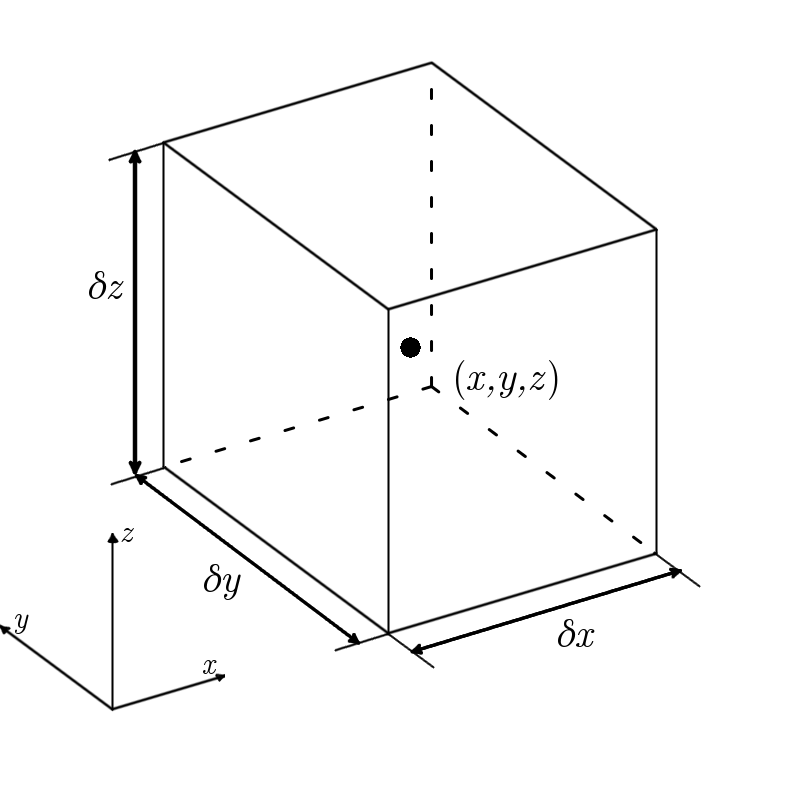
\includegraphics[width=8cm]{Img/1-1}
	\caption{Ilustración de un continuo}
	\label{img:1-1}
	\end{center}
\end{figure}

\subsection{Fluidos}

Un \textit{fluido} es una sustancia que se deforma continuamente cuando se le somete a un esfuerzo cortante, sin importar lo pequeño que sea el esfuerzo aplicado. De toda la gama posibles de fluidos se pueden agrupar o clasificar de acuerdo a diferentes criterios:

\begin{itemize}
	\item[$\bullet$] Laminar: El fluido se desplaza a bajas velocidades por capas, que deslizan una respecto de la otra de manera suave, en \textit{laminas} que no se mezclan entre si.
	\item[$\bullet$] Turbulento: Esta es una situación que no es estable, y la pérdida de estabilidad surge cuando los efectos inerciales (proporcionales al cuadrado de la velocidad) adquieren importancia relativa, de tal forma que el fluido comienza a moverse de manera caótica y desordenada, fenómeno que se incrementa a medida que el flujo tenga mayor velocidad.
	\item[$\bullet$] Compresible: Un fluido que presenta variaciones apreciables de la densidad.
	\item[$\bullet$] Incompresible: Fluido que mantiene su densidad constante.
\end{itemize}

\subsection{Principio de Conservación de la Masa}

Un cuerpo o volumen material ocupa una región del espacio (volumen) en un instante de tiempo $t$, el cual a medida que las partículas se desplazan a una velocidad $\mathbf{v}$, el cuerpo se deforma y pasa a ocupar otra región del espacio (Figura \ref{img:1-2}). A pesar de ello, el volumen material siempre posee el mismo conjunto de partículas, y como consecuencia, la masa que engloba el volumen es constante. Para un volumen arbitrario obtenemos:
\begin{equation}
	m = \int_{V_m (t)} \rho(t)dV, \nonumber
\end{equation}
donde $V_m(t)$ varía en el tiempo, entonces
\begin{equation}
	\frac{dm}{dt} = \frac{d}{dt} \int_{V_m (t)} \rho(t)dV = 0, \nonumber
\end{equation}
La cual constituye el denominado \textit{Principio de Conservación de la Masa}
\begin{figure}[htb]
    \begin{center}
      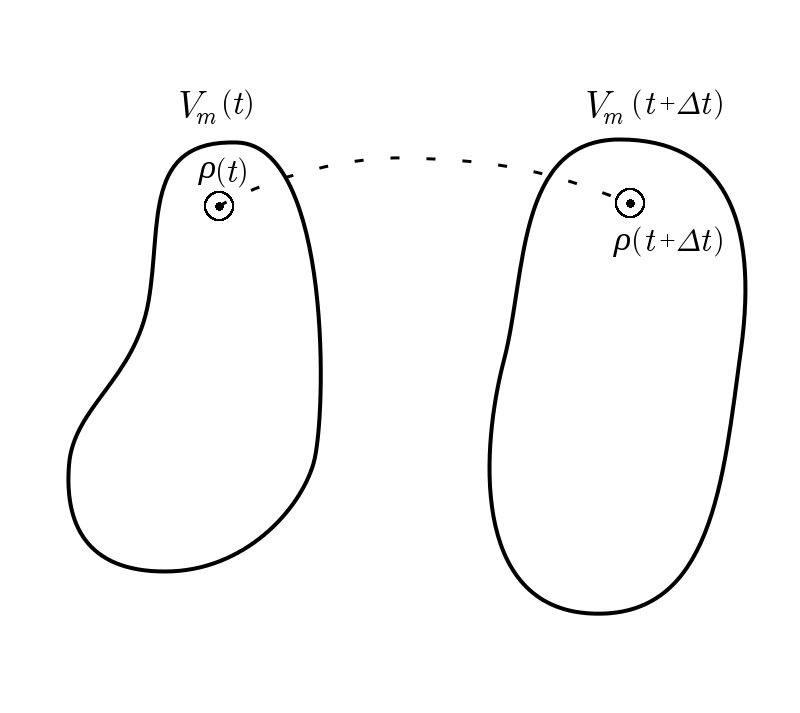
\includegraphics[width=8cm]{Img/1-2}
		\caption{Desplazamiento y deformación de un cuerpo}      
      \label{img:1-2}
    \end{center}
  \end{figure}

\subsection{Fuerzas de volumen y de superficie}

Definimos a la \textit{fuerza} como cualquier acción, esfuerzo o influencia que puede alterar el estado de movimiento o de reposo de cualquier cuerpo. Existen dos tipos de fuerza: de cuerpo o volumétricas y las de contacto o superficie. Las primeras actúan a distancia y sobre \textbf{todos} los elementos de volumen del material, sin la necesidad de tener un contacto directo con el cuerpo. Se representan mediante un campo vectorial \textbf{f} que determina la fuerza por masa unitaria, que al multiplicarlo por la densidad $\rho$ obtenemos la fuerza por volumen unitario y finalmente, al integrar en el volumen tenemos la fuerza que soporte dicho volumen. Un ejemplo claro es la gravedad:
\begin{equation}
	\mathbf{F}_V = \int_{V_m(t)} \rho \mathbf{g} dV. \nonumber
\end{equation}

El segundo grupo de fuerzas actúan en la superficie que limita al cuerpo arbitrario. Se ejerce por el contacto superficial entre el cuerpo y su vecindad asociada. Sea \textbf{n} un vector unitario normal a la superficie de interés, dirigido desde el cuerpo hacia el exterior; y $\mathbf{t}$ el \textit{vector de tensión}, fuerza por área unitaria que se le ejerce al cuerpo sobre la superficie de contacto. Establecemos que $\mathbf{t_{(n)}}$ representa la fuerza por unidad de área respecto de la normal.
\begin{equation}
	\mathbf{F}_S = \int_{A_m(t)} \rho \mathbf{t_{(n)}} dA. \nonumber
\end{equation}

\subsection{Principio de conservación del momento lineal}

En nuestro contexto de medios continuos, resulta más apropiado hablar de cantidad de movimiento que posee cada elemento diferencial de materia, cuya masa es $\rho dV$, por lo tanto el momento lineal de nuestro elemento está dado por $\rho \mathbf{v} dV$ y la cantidad de movimiento total es:
\begin{equation}
	\mathbf{p}(t) = \int_{V_m(t)} \rho \mathbf{v}dV. \nonumber
\end{equation}
Recordando la segunda ley de Newton, la cual establece que la sumatoria de las fuerzas que actúan sobre un cuerpo produce en él una aceleración tal que, multiplicada por su masa, es igual a la suma de las fuerzas actuantes. El equivalente de esta ley en la mecánica del continuo es el denominado \textit{Principio de conservación del momento lineal} y se expresa:
\begin{equation}
	\frac{d \mathbf{p}}{dt} = \mathbf{F}_v + \mathbf{F}S, \nonumber
\end{equation}
integrando en el volumen obtenemos
\begin{equation}
	\frac{d}{dt}	\int_{V_m(t)} \rho \mathbf{v} dV = \int_{V_m(t)} \rho \mathbf{g} dV + \int_{A_m(t)} \mathbf{t_{(n)}} dA,
	\label{eq:2-1}
\end{equation}
la cual expresa que la tasa temporal de cambio del momento lineal de un volumen es igual a la suma de las fuerzas de contacto y de volumen que actúan sobre el mismo.

\subsection{Estática de fluidos}

El término estática nos sugiere la noción de ``algo que está quiero" . Estática de fluidos refiere justamente al campo de estudio de los fluidos en reposo, en particular de las fuerzas actuantes, puesto que el fluido se encuentra en reposo, su velocidad y cantidad de movimientos son nulos. Por otro lado, si consideramos a la gravedad como la única fuerza de cuerpo, se tiene que $\mathbf{f} = \mathbf{g}$. En condiciones hidrostáticas, la única contribución al vector de tensión $ \mathbf{t_{(n)}}$ la provee la presión del fluido:
\begin{equation}
	\mathbf{t_{(n)}} = -p \mathbf{n}, \nonumber
\end{equation}
reemplazando en la ecuación \ref{eq:2-1} obtenemos
\begin{equation}
	0 = \int_{V_m} \rho \mathbf{g} dV - \int_{A_m} p \mathbf{n} dA. \nonumber
\end{equation}
Si aplicamos el teorema de la \textit{divergencia de Gaus} en el término de presión y despejando, 
\begin{equation}
	\rho  \mathbf{g} = \nabla p, \nonumber
\end{equation}
la cual expresa la \textit{Ecuación General de la Hidrostática}.

\section{Cinemática}

Como \textit{cinemática del continuo} entendemos que estudia la descripción y propiedades del movimiento de medios continuos, que a medida que se mueven y deforman \textit{transportan} diferentes propiedades (concentración, energía, cantidad de movimiento, etc.). Supongamos una región del espacio ($\Re^3$) en un determinado tiempo $t$, que contiene una cierta cantidad de materia ubicada en una posición $\mathbf{x}(t)$, las cuales se denominan \textit{coordenadas espaciales}. Si el material se estaba deformando, inicialmente parte de un estado o posición $\mathbf{a}(t_0)$ denominado estado de referencia, con el cual podemos identificar de manera única cada partícula por la posición que ocupaba, la que denominaremos \textit{coordenada material}.

Como el continuo está en movimiento, cualquier propiedad $\phi$ del mismo que se quiera evaluar cambiará con el tiempo. Para representar cualquier propiedad del continuo en movimiento, se pueden adoptar dos enfoques:
\begin{itemize}
	\item[$\bullet$] Medir la variación de la propiedad a medida que nos desplazamos con las partículas del continuo. En este caso, se debe representar la propiedad $\phi$ en función de las partículas del continuo y del tiempo ($\phi(\mathbf{a},t)$), este enfoque se denomina \textit{descripción Lagrangiana o material}.
	\item[$\bullet$] Medir la variación de la propiedad en posiciones determinadas del espacio, es decir, expresar la propiedad como función de las coordenadas espaciales y el tiempo ($\phi(\mathbf{x},t)$), este enfoque se denomina \textit{descripción Euleriana o espacial}.
\end{itemize}

Cabe aclarar que la propiedad $\phi$ no tendrá el mismo valor en la descripción material que en la espacial, ya que en la última se representa el valor de $\phi$ como función de la posición en el espacio y del tiempo; a medida que el continuo se mueve, una posición fija en el espacio será ocupada por diferentes partículas y por lo tanto con la descripción espacial no tenemos ninguna información \textit{directa} acerca de variación de propiedades de partículas. 

\section{Derivada material y derivada local}

Planteamos un ejemplo sencillo para introducir los términos de derivada material y local. Imaginemos que nos encontramos sobre un río en un bote con un sensor que determina la concentración de peses por volumen (c), inicialmente estamos con el bote anclado y el sensor registra la tasa de cambio temporal de la concentración de peses. Mide lo que se denomina \textit{derivada local} respecto del tiempo, $\partial c / \partial t$. Luego soltamos el ancla, dejando que la corriente arrastre al bote, moviéndonos a la velocidad del bote. El sensor continúa funcionando y sigue registrando la variación en la concentración de peces. Está midiendo lo que se conoce como \textit{derivada material} con respecto del tiempo de $c$, $Dc/Dt$. En ambos casos se cuantifica la velocidad de cambio de una variable de campo, pero sabemos que el significado físico de son diferentes. En el primero nos encontramos en una posición fija y en la segunda nos movemos a la velocidad del material.

Supongamos una partícula del material que identificamos mediante su coordenada material, la que mantendremos fija. A medida que transcurre el tiempo, esta partícula describe una trayectoria:
\begin{equation}
	\mathbf{x} = \left. \mathbf{x}(\mathbf{a},t) \right\vert_{\mathbf{a}_{fija}}. \nonumber
\end{equation}
El vector velocidad en el contexto del continuo, se define como la tasa de cambio de la posición espacial de una partícula material. De acuerdo con la anterior, esto es simplemente la derivada parcial de $\mathbf{x}$ respecto de $t$, manteniendo fijo $\mathbf{a}$:
\begin{equation}
	\mathbf{v} = \left. \frac{\partial \mathbf{x}}{\partial t} \right\vert_\mathbf{a}. \nonumber
\end{equation}

Cuando se calcula la derivada temporal de alguna propiedad manteniendo la partícula fija, es decir moviéndonos con la partícula misma, decimos que estamos calculando la derivada material del propiedad:
\begin{equation}
	\frac{D \phi}{D t} = \left. \frac{\partial \widehat{\phi}}{\partial t} \right\vert_{\mathbf{a}} ~~;~~ \phi = \widehat{\phi}(\mathbf{a},t). \nonumber
\end{equation}

Supongamos que $\phi$ está expresada en su descripción Euleriana teniendo sus valores como función de la posición ($\mathbf{x}$) y el tiempo ($t$). La derivada local de $\phi$ respecto del tiempo se obtiene al derivar manteniendo la posición $\mathbf{x}$ fija y se representa como:
\begin{equation}
	\left. \frac{\partial \phi}{\partial t} \right\vert_{\mathbf{x}}. \nonumber
\end{equation}

Para obtener la derivada material de $\phi$ utilizando una descripción Euleriana, debemos derivar siguiendo el movimiento de la partícula determinada. Dado que $\phi = \phi(\mathbf{x},t) = \phi [\mathbf{x}(\mathbf{a},t),t]$, la derivada espacial de esta variable respecto del tiempo se obtiene mediante la regla de la cadena:
\begin{equation}
	\left. \frac{\partial \phi}{\partial t} \right\vert_\mathbf{a} = \left. \frac{\partial \phi}{\partial t} \right\vert_\mathbf{x} + \left. \frac{\partial \phi}{\partial x} \right\vert_t \left. \frac{\partial x}{\partial t} \right\vert_\mathbf{a}, \nonumber 
\end{equation}
donde $\partial \phi / \partial x = \nabla \phi$ y $\partial x /\partial t = \mathbf{v}$, entonces reescribiendo la ecuación, obtenemos:
\begin{equation}
	\frac{D\phi}{Dt} = \frac{\partial \phi}{\partial t} + \mathbf{v} \cdot \nabla \phi.
	\label{eq:2-2}
\end{equation}
Esto es, para calcular la tasa temporal de cambio de una propiedad descripta en forma euleriana a medida que nos desplazamos a la velocidad del fluido ($\mathbf{v}$), debemos adicionar a la derivada local, un término denominado \textit{convectivo}. Dicho término tiene en cuenta la variación temporal que experimenta la partícula al moverse con la velocidad $\mathbf{v}$ en un campo no uniforme en el espacio.

\section{Tensiones}

Un término que hemos mencionado pero no profundizado es el de \textit{tensión}, el cual representa la interacción entre dos partes a través de la superficie límite entre las regiones y se expresan como fuerzas por unidad de superficie.

Supongamos un material $B$ que ocupa un volumen $V$, enfocándonos en la superficie $\Delta S$ con una normal $\mathbf{n}$, como lo muestra la figura \ref{img:1-3}.
\begin{figure}[h!]
    \centering
    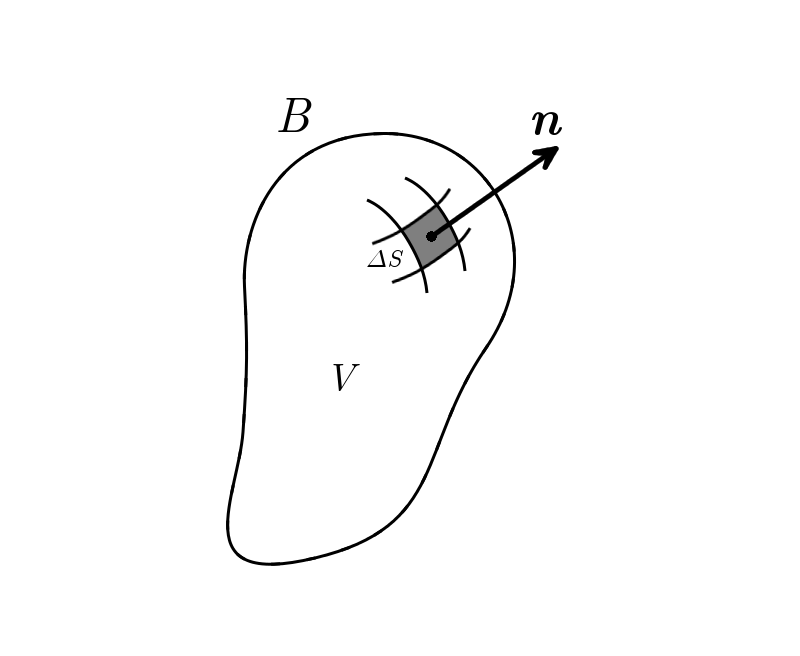
\includegraphics[width=8cm]{Img/1-3}
	\caption{Superficie de interés en B con normal \textbf{n}}      
    \label{img:1-3}
\end{figure}

A partir de la dirección de $\mathbf{n}$ podemos distinguir dos lados de $\Delta S$, consideremos que la parte positiva del material (exterior), ejerce una fuerza $\Delta F$ sobre la parte negativa. La fuerza depende de la ubicación, del tamaño de $\Delta S$ y de la dirección $\mathbf{n}$, entonces
\begin{equation}
	\Delta F = f (\mathbf{x},\Delta S, \mathbf{n}), \nonumber
\end{equation}
además asumimos que:
\begin{itemize}
	\item[$\bullet$] Cuando $\Delta S \rightarrow 0$, la relación $\Delta F / \Delta S$ tiende a un valor límite de \textit{tracción de superficie} o \textit{vector de tensión}.
	\begin{equation}
		\frac{dF}{dS}  = t_{(\mathbf{n})}. \nonumber
	\end{equation}
	\item[$\bullet$] El momento de la fuerza $\Delta F$ en torno a cualquier punto dentro de $\Delta S$ es cero en el límite $\Delta S \rightarrow 0$,
\end{itemize}
ambas consideraciones se conocen como el \textit{principio de Euler y Cauchy}.

Supongamos un continuo cartesiano donde cada cara $\Delta S_i$ están sujetas a tensiones $t_i = \left\lbrace t_{i1},t_{i2},t_{i3} \right\rbrace$ y sus normales son paralelas a los ejes de coordenadas $(x_1,x_2,x_3)$. Si concatenamos los componentes de tension actuando sobre las tres caras obtenemos una matriz cuadrada, la cual se denomina como el \textit{tensor de tensiones}:
\begin{equation}
	\tau = 
	\begin{bmatrix}
		t_{11} && t_{12} && t_{13} \\
		t_{21} && t_{22} && t_{23} \\
		t_{21} && t_{32} && t_{33} \\
	\end{bmatrix} \nonumber
\end{equation}
donde las componentes $t_{ii}$ son denominadas como \textit{tensiones principales} y el resto, \textit{tensiones de corte}.

Para un tensor de tensiones $\tau$ conocido, podemos obtener la tensión que está actuando sobre una superficie multiplicando el tensor por la normal $n_{ds}$ de dicha superficie 
\begin{equation}
	t_{n_{ds}} = \tau n_{ds}, \nonumber
\end{equation}
esta ecuación se define como la \textit{ecuación de Cauchy}.

\subsection{Ecuación de equilibrio}

Consideramos un continuo con dimensiones infinitesimales ($dx,dy,dz$) con sus ejes paralelos a los cartesianos. Las tensiones que actúan sobre él se muestran en la figura \ref{img:1-4}, por ejemplo la fuerza que actúa sobre el lado izquierdo es:
\begin{figure}[h!]
    \centering
    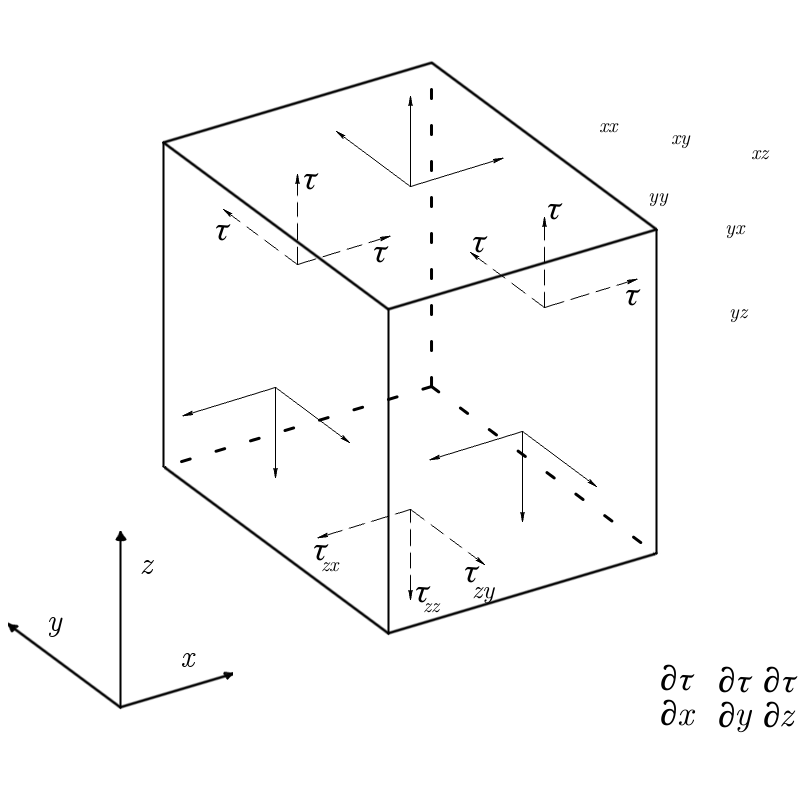
\includegraphics[width=8cm]{Img/1-4}
	\caption{Tensiones sobre un Continuo}
	\label{img:1-4}
\end{figure}

\begin{equation}
	\tau_{11} dy dz, \nonumber
\end{equation} 
la fuerza que actúa sobre la cara derecha se obtuvo utilizando el \textit{teorema de Taylor}:
\begin{equation}
	\left( \tau_{11} + \frac{\partial \tau_{11}}{\partial x} dx \right) dy dz, \nonumber
\end{equation} 
etc. La suma de todas las componentes de fuerzas en el eje $x$ esta dado por:
\begin{eqnarray}
	F_x = \left( \tau_{11} + \frac{\partial \tau_{11}}{\partial x} dx \right) dy dz - \tau_{11} dy dz \nonumber \\
		+ \left( \tau_{21} + \frac{\partial \tau_{21}}{\partial y} dy \right) dx dz - \tau_{21} dx dz \nonumber \\
		+ \left( \tau_{31} + \frac{\partial \tau_{31}}{\partial z} dz \right) dx dy - \tau_{31} dx dy \nonumber \\
		+ X_x dx dy dz. \nonumber
\end{eqnarray}
Si el cuerpo está en equilibrio sabemos que $F_x = 0$ y al dividir la ecuación anterior por el volumen ($dxdydz$) obtenemos:
\begin{equation}
	\frac{\partial \tau_{11}}{\partial x} + \frac{\partial \tau_{21}}{\partial y} + \frac{\partial \tau_{31}}{\partial z} + X_x = 0. \nonumber
\end{equation}
De manera general obtenemos:
\begin{equation}
	\nabla \cdot \tau + X = 0. \nonumber
\end{equation}

Un elemento en equilibrio requiere que las fuerzas resultantes sean nulas y que no existan momentos externos, por lo tanto obtenemos que el \textit{tensor de tensiones es simétrico},
\begin{equation}
	\tau_{ij} = \tau_{ji}. \nonumber
\end{equation}

A modo general, un cuerpo está en equilibrio si $\nabla \cdot \tau + X = 0$ y $\tau_{ij} = \tau_{ji}$.

\section{Conservación de masa y ecuación de continuidad}

Hemos defino el principio de conservación de masa y su expresión matemática integral para un volumen material, ahora aplicamos el \textit{Teorema de Transporte de Reynolds} con $\mathbf{w} = \mathbf{v}$, siendo 
$\mathbf{v}$ la velocidad con la que se desplaza el material:
\begin{equation}
	\frac{d}{dt} \int_v \rho dV = \int_V \left[ \frac{\partial \rho}{\partial t} + \nabla \cdot (\rho \mathbf{v}) \right] dV = 0, \nonumber
\end{equation}
dado que esta ecuación es válida para cualquier volumen, el integrando debe ser nulo:
\begin{equation}
	\frac{\partial \rho}{\partial t} + \nabla \cdot (\rho \mathbf{v}) = 0.
	\label{eq:2-3}
\end{equation}
La expresión \ref{eq:2-3} se denomina \textit{ecuación de continuidad}, válida localmente en cualquier punto de un medio continuo. Utilizando la definición de derivada material, podemos expresarla:
\begin{equation}
	\frac{D \rho}{D t} + \nabla \cdot (\rho \mathbf{v}) = 0. \nonumber
\end{equation}
Nótese que si $\rho = cte.$ el \textit{fluido es incompresible} ó si $D \rho / Dt = 0$ el flujo es \textit{barotrópico}, y la ecuación de continuidad resulta:
\begin{equation}
	\nabla \cdot \mathbf{v} = 0.
	\label{eq:2-4}
\end{equation}
Si bien para ambos fluidos la ecuación de continuidad es igual, cabe diferenciarlos ya que para un fluido incompresible la densidad es constante e independiente del tiempo y de su posición, en cambio un flujo barotrópico la densidad de una partícula es constante a medida que se desplaza.

\section{Ecuación diferencial del Movimiento}

Partiendo de la ecuación de conservación del momento lineal \ref{eq:2-1} y aplicando la ecuación de Cauchy ($\mathbf{t_{(n)}} = \tau \mathbf{n}$) obtenemos:
\begin{equation}
	\frac{D}{Dt} \int_V \rho \mathbf{v} dV = \int_V \rho \mathbf{g} dV + \int_A \tau \cdot \mathbf{n} dA, \nonumber
\end{equation}
luego aplicando el teorema de la divergencia en el término derecho y despejando obtenemos:
\begin{eqnarray}
	\frac{D}{Dt} \int_V \rho \mathbf{v} dV = \int_V \rho \mathbf{g} dV + \int_V \nabla \cdot \tau dV, \nonumber \\
	\int_V \left( \rho \frac{D \mathbf{v}}{Dt} - \rho \mathbf{g} - \nabla \cdot \tau  \right) dV = 0. \nonumber
\end{eqnarray}
Dado que el volumen del material puede ser arbitrario, necesariamente el integrando debe ser nulo,
\begin{equation}
	\rho \frac{D \mathbf{v}}{Dt} = \rho \mathbf{g} + \nabla \cdot \tau.
	\label{eq:2-5}
\end{equation}
Básicamente esta ecuación expresa la segunda ley de Newton y la denominaremos \textit{Balance Diferencial de Cantidad de Movimiento}.

\section{Tensor de Tensiones Viscosas}

Cuando un fluido se encuentra en movimiento, surgen tensiones adicionales a las hidrostáticas, originadas en las deformaciones que se producen en el medio continuo. El tensor que incluye todos los efectos se denomina el \textit{Tensor de Tensiones Viscosas} $T_v$:
\begin{equation}
	T_v = \tau - p \mathbf{I}, \nonumber
\end{equation}
donde $\mathbf{I}$ es la matriz identidad y $\tau$ el tensor de fuerzas viscosas. Introduciendo este concepto en \ref{eq:2-5} obtenemos:
\begin{equation}
	\rho \frac{D \mathbf{v}}{Dt} = \rho \mathbf{g} -\nabla p + \nabla \cdot \tau,
	\label{eq:2-6}
\end{equation}
donde $\tau$ depende de las deformaciones del medio continuo, las ecuaciones que expresan esta dependencia se conocen como las \textit{Ecuaciones Constitutivas}.

\subsection{Ley de la viscosidad de Newton}

Analicemos la situación de la figura \ref{img:1-5},
\begin{figure}[h!]
	\centering
	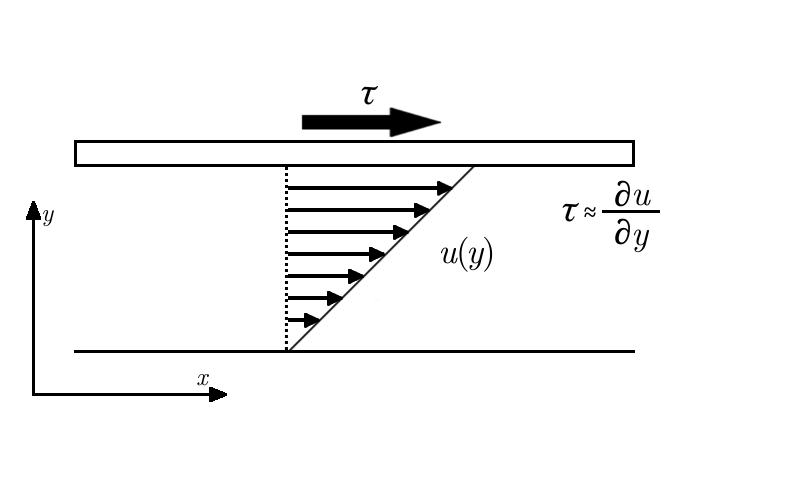
\includegraphics[width=8cm]{Img/1-5}
	\caption{Fluido viscoso confinado entre dos placas paralelas}
	\label{img:1-5}
\end{figure}
donde existe un ``fluido viscoso" $~$confinado entre dos placas planas paralelas. Si se aplica una fuerza tangencial a estas placas, se produciría un movimiento relativo entre las mismas. En la situación particular que estamos analizando, el perfil de velocidades dentro del canal tiene una forma lineal como la que se muestra, donde se ha supuesto que una de las placas está fija mientras la otra se mueve. Podemos entonces caracterizar la deformación del líquido mediante la pendiente del perfil de velocidades, es decir $\partial v_x / \partial y$. A medida que el movimiento relativo es mayor y en consecuencia la velocidad de deformación es mayor, el valor de la derivada incrementa:
\begin{equation}
	\tau = \mu \frac{\partial v_x}{\partial y}, \nonumber
\end{equation}
la cual define la relación de proporcionalidad entre velocidad de deformación y tensión viscosa.

Un fluido Newtoniano es un tipo idealizado de fluido que reúne las siguientes características:
\begin{itemize}
	\item[$\bullet$] Las componentes del Tensor de Tensiones Viscosas  \textbf{dependen linealmente} de las componentes del Tensor Tasa de Deformación.
	\item[$\bullet$] Es un fluido isotrópico, es decir, que sus propiedades son independientes de la orientación con la que se las examine.
\end{itemize}

La ecuación más general que cumple con estos requisitos puede escribirse:
\begin{equation}
	\tau = (\kappa - 2/3 \mu) (\nabla \cdot \mathbf{v}) \mathbf{I} + \mu [\nabla \mathbf{v} + \nabla (\mathbf{v})^T], \nonumber
\end{equation}
donde $\kappa$ y $\mu$ son conocidas como \textit{viscosidad dilatacional} y \textit{viscosidad de corte} respectivamente. Introduciendo estas expresiones en la ecuación \ref{eq:2-6} obtenemos:
\begin{equation}
	\rho \frac{D \mathbf{v}}{Dt} = \rho \mathbf{g} -\nabla p + \nabla \cdot \left[ \left( \kappa - \frac{2}{3} \mu \right) \left( \nabla \cdot \mathbf{v} \right) \mathbf{I} + \mu \left( \nabla \mathbf{v} + \nabla \mathbf{v}^T \right) \right]. \nonumber
\end{equation}
\begin{equation}
	\rho \left( \frac{\partial \mathbf{v}}{\partial t} + \mathbf{v} \cdot \nabla \mathbf{v} \right) = \rho \mathbf{g} -\nabla p + \nabla \left[ \left( \kappa - \frac{2}{3} \mu \right) \left( \nabla \cdot \mathbf{v} \right)\right] + \nabla \cdot \left[ \mu \left( \nabla \mathbf{v} + \nabla \mathbf{v}^T \right) \right]. \nonumber
\end{equation}

Si los coeficientes de viscosidad ($\kappa$ y $\mu$) son constantes, desarrollamos:
\begin{equation}
	\rho \left( \frac{\partial \mathbf{v}}{\partial t} + \mathbf{v} \cdot \nabla \mathbf{v} \right) = \rho \mathbf{g} -\nabla p + \left( \kappa - \frac{2}{3} \mu \right) \nabla \left( \nabla \cdot \mathbf{v} \right) + \mu \left[ \nabla \cdot \left( \nabla \mathbf{v} \right) + \nabla \cdot \left( \nabla \mathbf{v}^T \right) \right]. \nonumber
\end{equation}
\begin{equation}
	\rho \left( \frac{\partial \mathbf{v}}{\partial t} + \mathbf{v} \cdot \nabla \mathbf{v} \right) = \rho \mathbf{g} -\nabla p + \left( \kappa - \frac{2}{3} \mu \right) \nabla \left( \nabla \cdot \mathbf{v} \right) + \mu \left[\Delta \mathbf{v} + \nabla \left( \nabla \cdot \mathbf{v} \right) \right]. \nonumber
\end{equation}
\begin{equation}
	\rho \left( \frac{\partial \mathbf{v}}{\partial t} + \mathbf{v} \cdot \nabla \mathbf{v} \right) = \rho \mathbf{g} -\nabla p + \left( \kappa + \frac{1}{3} \mu \right) \nabla \left( \nabla \cdot \mathbf{v} \right) + \mu \Delta \mathbf{v}. \nonumber
\end{equation}

Finalmente si el fluido es incompresible:
\begin{equation}
	\rho \left( \frac{\partial \mathbf{v}}{\partial t} + \mathbf{v} \cdot \nabla \mathbf{v} \right) = \rho \mathbf{g} -\nabla p + \mu \Delta \mathbf{v}.
	\label{eq:2-7}
\end{equation}

La ecuación \ref{eq:2-7} se conoce como la \textit{Ecuación de Navier-Stokes}, y es una de las ecuaciones fundamentales de la Mecánica de Fluidos. Esta ecuación es válida para un fluido Newtoniano e incompresible de viscosidad constante, junto a la ecuación de continuidad para un fluido incompresible ($\nabla \mathbf{v} = 0$), forman el sistema de ecuaciones diferenciales en derivadas parciales \textbf{no-lineales} para las incógnitas $p$ y $v_i$.

\chapter{Discretización Espacial}

Una vez resuelto el modelo matemático que describe el comportamiento del problema a resolver, el siguiente paso es aproximar el dominio del continuo (espacio y tiempo) con una representación discreta (nodos o subdominios), en el cual las variables desconocidas son determinadas. Usualmente la discretización de la representación geométrica toma la forma de una grilla sobre el dominio del problema. En la práctica existen muchas geometrías complejas (turbinas, aeroplanos, etc.), para las cuales, generar una grilla puede consumir mucho tiempo computacional, además la calidad de la grilla generada afecta directamente al método de simulación en puntos delicados como la estabilidad, tiempo de convergencia, eficiencia, etc., es por esto, que la generación de grillas es una práctica con alto interés.

\section{Geometría del Problema}

Un aspecto importante al momento de aplicar métodos numéricos a problemas concretos, es definir la geometría del problema, es decir, como se define y como se representa matemáticamente en la computadora. Actualmente en la práctica de ingeniería la información que representa la geometría se dispone en un formato estandarizado, 
\begin{figure}[b!]
	\centering
	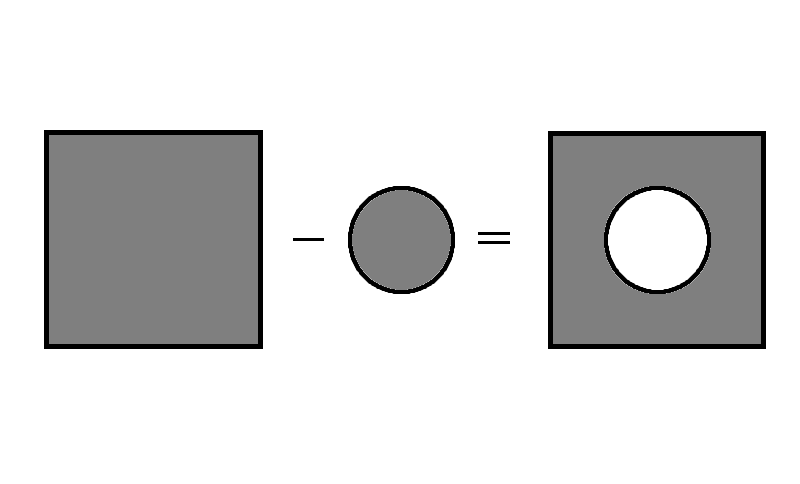
\includegraphics[width=8cm]{Img/3-1}
	\caption{Resta boleana entre un cuadrado y un círculo}
	\label{img:3-1}
\end{figure}
el cual puede ser generado por sistemas CAD. Existen diversas técnicas para describir la geometría, nombramos las principales:
\begin{itemize}
	\item[$\bullet$] modelado de volumen,
	\item[$\bullet$] modelado de contorno.
\end{itemize}

El modelado de volumen esta basado en la definición de objetos simples (cubos, cilindros, esferas, etc), los cuales son combinados utilizando operaciones algebraicas del tipo booleanas. Por ejemplo, un cuadrado hueco puede ser representado aplicando la resta entre un cuadrado y un circulo como lo muestra la figura \ref{img:3-1}.

El método más utilizado para describir la geometría es por la representación de superficies de contorno (casos tridimensionales) o curvas de contorno (casos bidimensionales). Dicha descripción consiste en una composición de superficies o curvas las cuales representan el contorno del dominio, figura \ref{img:3-2}:
\begin{figure}[h!]
	\centering
	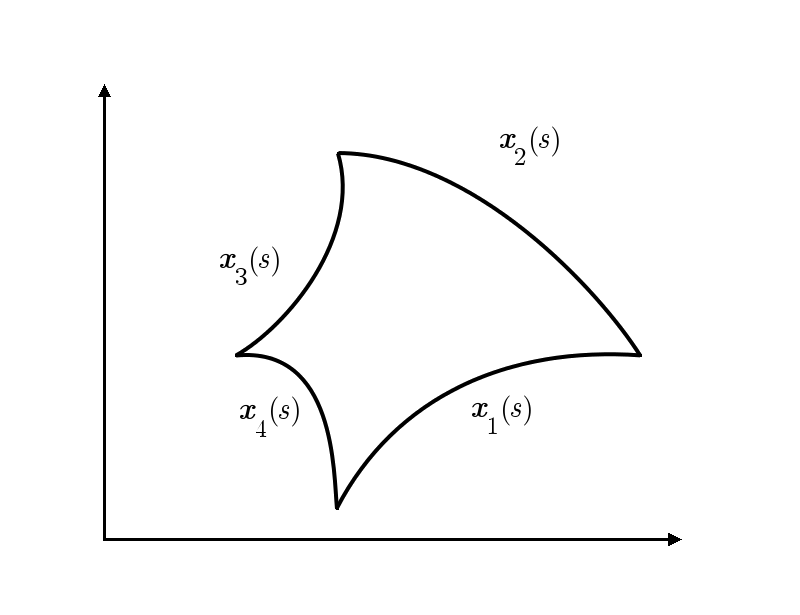
\includegraphics[width=8cm]{Img/3-2}
	\caption{Contorno formado por curvas $x_1$ $x_2$ $x_3$ $x_4$}
	\label{img:3-2}
\end{figure}

Las superficies o curvas usualmente son definidas por funciones \textit{B-splines} o por \textit{curvas de Bezier}. Las curvas de Bezier utiliza como parámetros puntos de control (\textbf{$b_i$}) con sus respectivas funciones de peso (\textbf{$B^n_i(s)$}) denominadas como los  \textit{polinomios de Bernstein}.
\begin{equation}
	x(s) = \sum^n_{i=0} b_i B^n_i(s)
\end{equation}
Donde $x(s)$ es la curva de Bezier con n+1 puntos de control. 

En la figura \ref{img:3-3} mostramos un ejemplo de una curva de Bezier de orden 4:
\begin{figure}[h!]
	\centering
	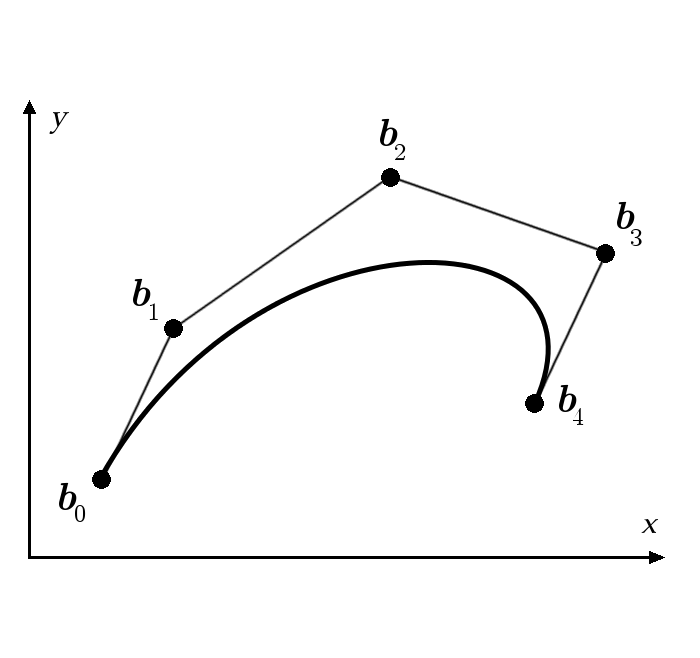
\includegraphics[width=8cm]{Img/3-3}
	\caption{Curva de Bezier de 4to orden}
	\label{img:3-3}
\end{figure}

\pagebreak

\section{Grilla}

Todos los métodos de discretización, como los que explicaremos en capítulos siguientes, requieren como primera instancia, una discretización espacial del dominio del problema. Una grilla está definida por celdas, las cuales en dos dimensiones están formadas por lineas, en tres dimensiones se forman utilizando superficies, que a su vez son formadas por lineas. La intersección de las lineas son definidas como puntos de la grilla (Figura \ref{img:3-4}).
\begin{figure}[h!]
	\centering
	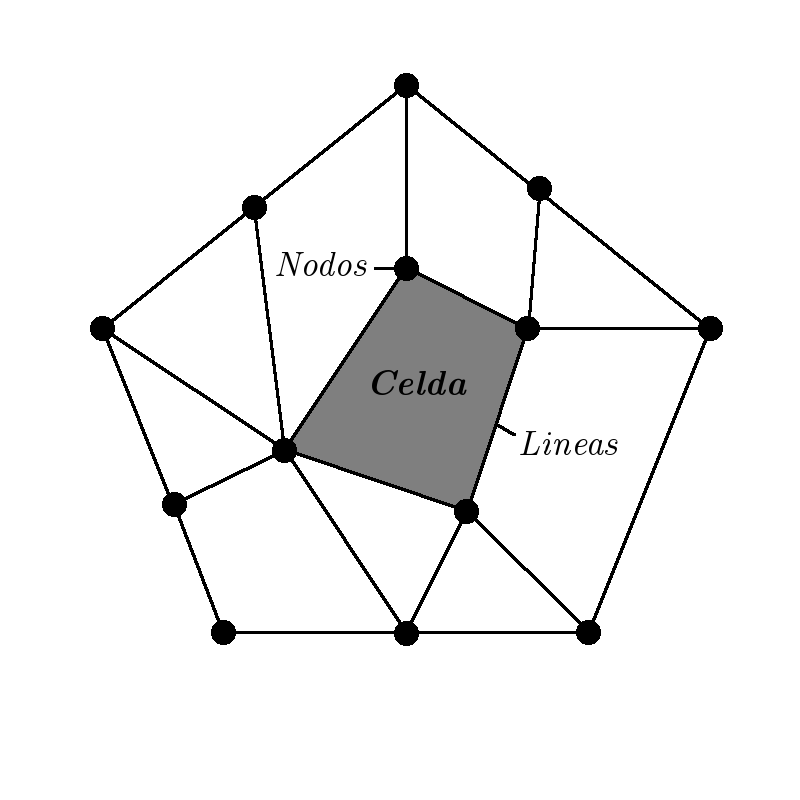
\includegraphics[width=7cm]{Img/3-5}
	\caption{Elementos de una grilla}
	\label{img:3-4}
\end{figure}

En la práctica, la generación de una grilla para problemas de geometría compleja es lo que más costo computacional tiene. Por un lado, la grilla debe modelar la geometría lo más exacto posible, por el otro, la grilla debe ser ``buena" respecto eficiencia y aproximación. Aquí debemos tener en cuenta la interacción entre la geometría discretizada, la discretización de las ecuaciones y la solución del método, de manera general: \\

\textit{Mientras mas regular sea la grilla, mayor sera la eficiencia de la solución generada por el algoritmo computacional, pero es menos inflexible a la hora de modelar geometrías complejas} \\

Por lo tanto, es necesario encontrar un equilibrio donde se analicen los requerimientos concretos del problema que se está por resolver. Entonces la generación de la grilla debe tener límites; un caso particular, es un problema temporal en el cual, la grilla sufre modificaciones o debe generarse para cada instante de tiempo, lo que agrega un costo computacional importante.

\subsection{Tipo de grillas}

El tipo de grilla está muy relacionada al tipo de discretización y a las técnicas de solución utilizadas en la computación.

Una primera clasificación está dada por la forma de las celdas. El caso más sencillos es el unidimensional, el cual, solo depende de los intervalos; en dos-dimensiones las celdas pueden tomar la forma de triángulos o cuadriláteros, y tetraedros, hexaedros, prismas o pirámides para el caso tridimensional.

Las grillas se clasifican en los siguientes tipos (Figura \ref{img:3-5}):
\begin{itemize} 
	\item[$\bullet$] grillas de contorno,
	\item[$\bullet$] grillas Cartesianas,
	\item[$\bullet$] grillas superpuestas.
\end{itemize}
\begin{figure}[h!]
	\centering
	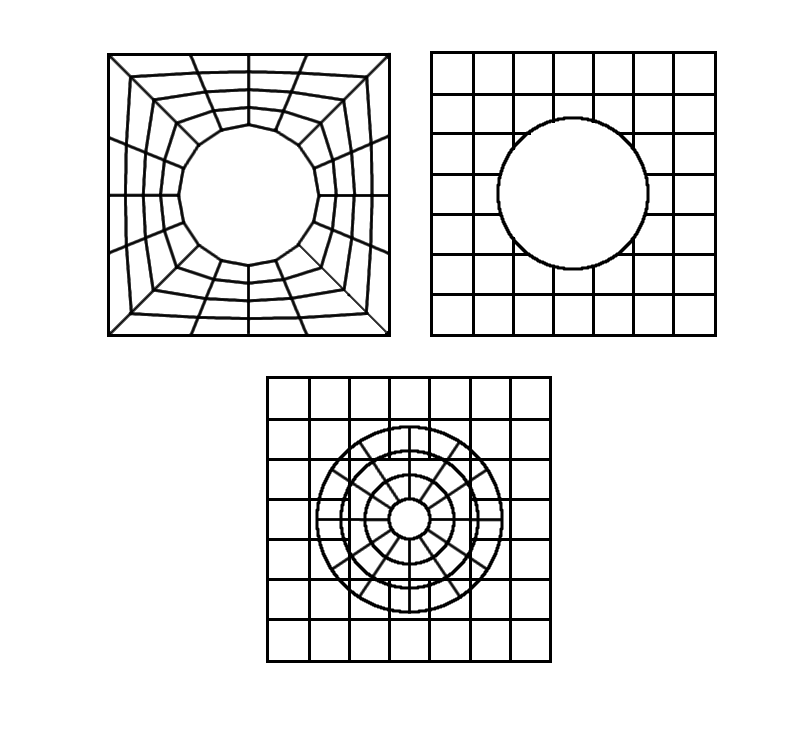
\includegraphics[width=6.5cm]{Img/3-6}
	\caption{(a) Grillas de contornos, (b) cartesianas y (c) superpuestas}
	\label{img:3-5}
\end{figure}
Las grillas de contorno se caracterizan por utilizar lineas o superficies con el objetivo de aproximar el contorno del dominio. Las cartesianas aproximan el contorno del dominio con grillas regulares, esto provoca realizar un tratamiento especial para contornos irregulares. Por último, las grillas superpuestas discretizan diferentes regiones del dominio de manera independiente una de las otras, utilizando grillas regulares permitiendo que se superpongan y realizando un tratamiento especial en dichas áreas. 

\subsection{Estructura de la grilla}

Las grillas se clasifican según el tipo de celdas que contienen, de manera general, pueden ser clasificadas en dos tipo:
\begin{itemize} 
	\item[$\bullet$] grillas estructuradas (Figura \ref{img:3-6}),
	\item[$\bullet$] grillas no-estructuradas (Figura \ref{img:3-7}).
\end{itemize}

Las grillas estructuradas se caracterizan por tener una distribución regular de las celdas. Lo cual permite acceder fácilmente a los vecinos ($i+-1,j+-1$) de un elemento ($i,j$) en particular, realizando un desplazamiento $dx$ o $dy$ conocido. Este tipo de mallas son fáciles de generar y ocupan poca memoria, pero como gran desventaja es que no pueden adaptarse a geometrías complicadas y complejas, lo que las hacen poco atractiva. 
\begin{figure}[h!]
	\centering
	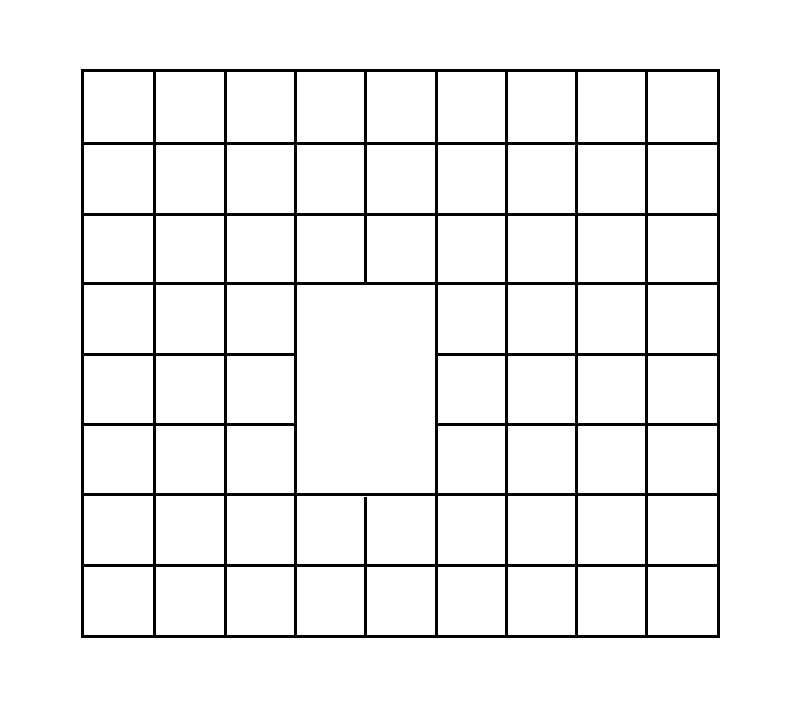
\includegraphics[width=8cm]{Img/3-7}
	\caption{Grilla estructurada con elementos cuadrados}
	\label{img:3-6}
\end{figure}

En las grillas no-estructuradas evitan utilizar celdas distribuidas de manera regular, dando la posibilidad de organizar los puntos de forma arbitraria sobre el dominio del problema, brindando una mejor flexibilidad, ya que las celdas pueden adaptarse de manera óptima a contornos complejos que deban analizarse. Debido a esto la relación de vecindad entre los elementos debe ser almacenada, además que requieren un algoritmo para ser generadas aumentando su costo computacional.
\begin{figure}[h!]
	\centering
	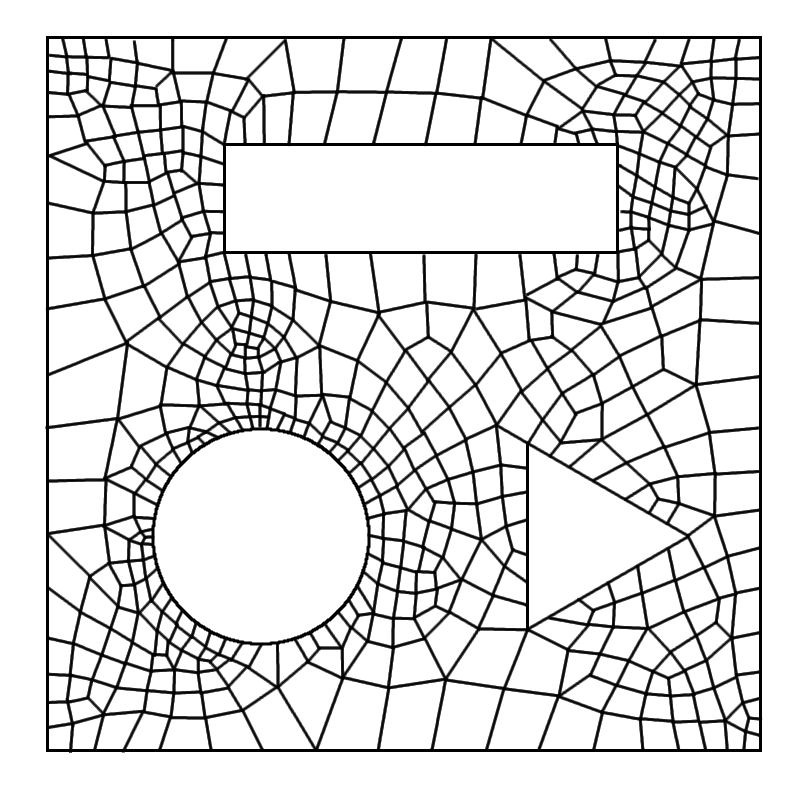
\includegraphics[width=8cm]{Img/3-8}
	\caption{Grilla no-estructurada con elementos cuadrados}
	\label{img:3-7}
\end{figure}

El cuadro \ref{tabla1} realiza una comparación de las diversas propiedades de las grillas:

$ \ $ 
\begin{table}[h!]
\centering
\begin{tabular}{| l c c |}
	\hline
	Propiedades & Estructurado & No-estructurado \\
	\hline
	Modelar geometrías complejas & - & + \\
	Automatizar la generación de la grilla & - & + \\
	Adaptación local al refinamiento de la grilla & - & + \\	
	Costo de generación de grilla & + & - \\
	Costo de programación & + & - \\
	Almacenamiento y direccionamiento & + & - \\
	Paralelización & + & - \\
	\hline	
\end{tabular}
\caption{Propiedades de las grillas estructuradas y no-estructuradas}
\label{tabla1}
\end{table}
\chapter{Volúmenes Finitos}
%\addcontentsline{toc}{chapter}{Volúmenes Finitos}

Luego de discretizar la geometría, continuamos con la elección del método que discretize las ecuaciones de gobierno, de cuales podemos distinguir dos grandes ramas: los que resuelven las ecuaciones diferenciales discretizando las derivadas, utilizando la serie de Taylor para obtener una aproximación a las derivadas primeras, segundas, etc. y se implementan bajo el uso de mallas estructuradas con desplazamientos $dx$, $dy$ y $dz$ constantes, de otra manera se deben realizar las correcciones necesarias; y los métodos que resuelven las ecuaciones integrando en los sub-dominios denominados elementos o volúmenes con la particularidad que pueden ser implementados para cualquier tipo de malla. 

En el segundo grupo se encuentra el Método de Volúmenes Finitos (MVF), el cual es principalmente utilizado para resolver problemas de mecánica de fluidos y posee una particularidad que lo hace especialmente atractivo: la ``conservación de los flujos numéricos" de manera local. Este método es localmente conservativo porque está basado en un enfoque de ``balance", donde cada elemento de la discretización plantea su propia ecuación de balance local respecto a sus vecinos, realizando una formulación basada en los flujos en su frontera.

\section{Metodología}

El MVF involucra los siguientes pasos:
\begin{itemize} 
	\item[$\bullet$] Descomposición del dominio en volúmenes de control.
	\item[$\bullet$] Formular las ecuaciones de balance de manera integral para cada volúmen de control.
	\item[$\bullet$] Aproximar las integrales de superficie y volumétricas.
	\item[$\bullet$] Aproximar las funciones y derivadas interpolando.
	\item[$\bullet$] Ensamblar y resolver el sistema algebraico.
\end{itemize}
y utilizaremos la ecuación \ref{eq:4-1} para ejemplificar sobre un dominio $\omega$.
\begin{equation}
	\frac{\partial}{\partial x_i} \left( \rho v_i \phi - k \frac{\partial \phi}{\partial x_i} \right) = f
	\label{eq:4-1}
\end{equation}

El primer paso en el MVF es discretizar o descomponer el dominio $\Omega$ en un número finito de subdominios $V_i (i=1,...,N)$, denominados \textit{volúmenes de control} (VC), y relacionarlos con los nodos donde se encuentran las variables a calcular, donde la unión es el dominio del problema sin superposición, es decir, su intersección es nula. Cada VC genera su propia ecuación de balance en relación con sus vecinos y el contorno, las cuales en su conjunto representan el sistema de ecuaciones a resolver.

Para problemas unidimensionales los VC son subintervalos ($dx$) y los nodos pueden ser los centroides o el contorno como lo muestra la figura \ref{img:4-1}:
\begin{figure}[h!]
	\centering
	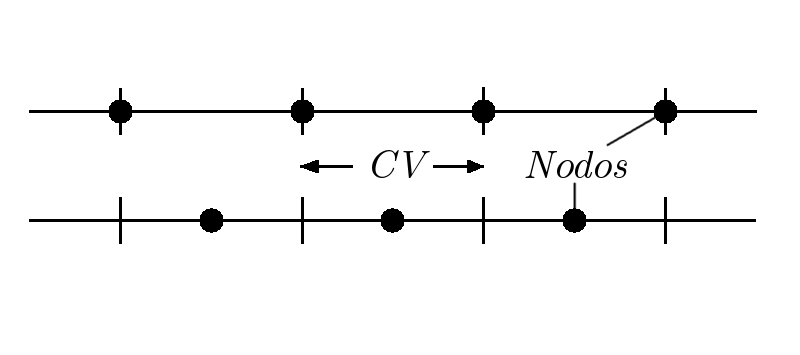
\includegraphics[width=8cm]{Img/4-1}
	\caption{Volúmenes de control}
	\label{img:4-1}
\end{figure}

Al extendernos a dos dimensiones, los VC pueden ser polígonos arbitrarios y los nodos se definen en los vértices o en el centro de los VC, estos enfoques se denominan centrados en el vértice o en la celda respectivamente (Figura \ref{img:4-2}). 
\begin{figure}[h!]
	\centering
	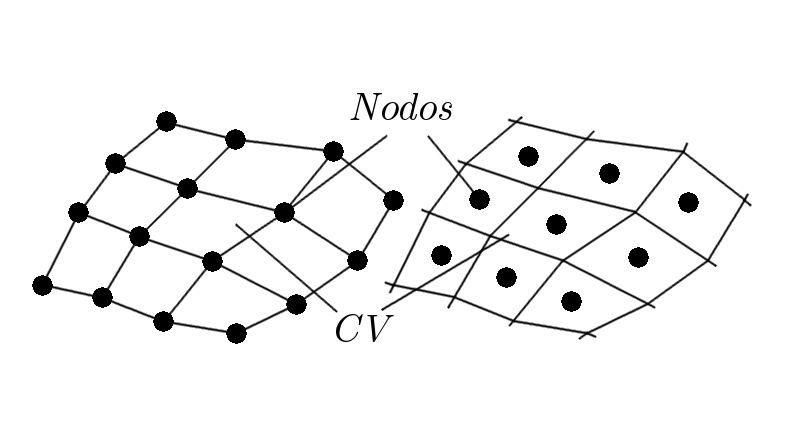
\includegraphics[width=8cm]{Img/4-2}
	\caption{Volúmenes de control 2D}
	\label{img:4-2}
\end{figure}
Para mallas con celdas triangulares, los nodos puede ser los vértices o centros de los triángulos, que definen los VC. Un enfoque es utilizar la triangulación de Delaunay, donde los nodos son se definen en el vértice de los triángulos y los VC como el polígono que forman las bisectrices de los triángulos al que pertenece dicho vértice (ver figura \ref{img:4-3}). Estos políginos se denominan los \textit{poligonos de Voronoi} los cuales para dominios convexos y sin triángulos obtusos presentan ``buenas" $~$ propiedades. 
\begin{figure}[h!]
	\centering
	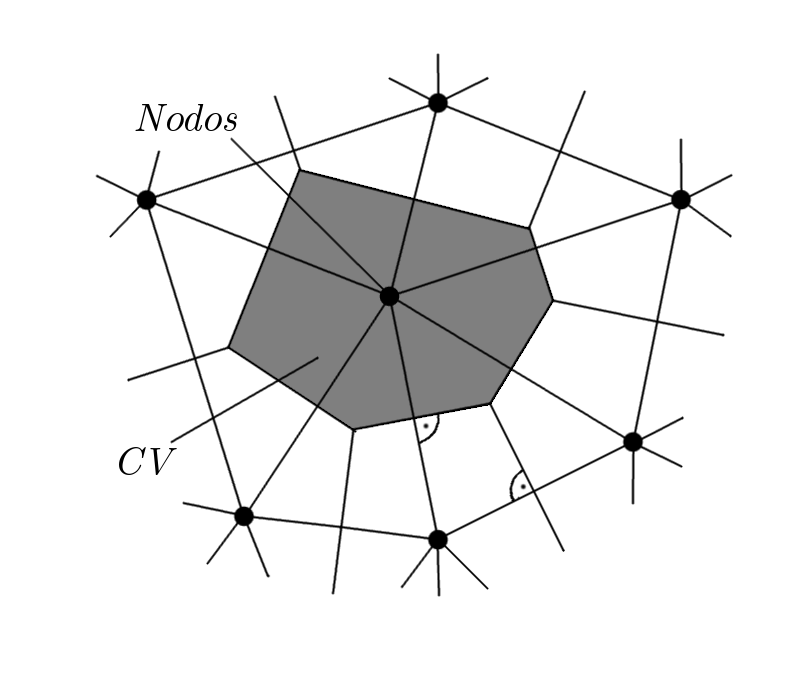
\includegraphics[width=8cm]{Img/4-3}
	\caption{Poligonos de Voronoi}
	\label{img:4-3}
\end{figure}

\pagebreak 

Utilizando la misma base con el enfoque centrado en la celda, podemos definir al nodo como la intersección de las bisectrices de los segmentos que conforman el VC triángular como lo muestra la figura \ref{img:4-32}, este enfoque tiene propiedades similares que los polígonos de Voronoi y presenta dificultades ante triángulos obtusos.
\begin{figure}[h!]
	\centering
	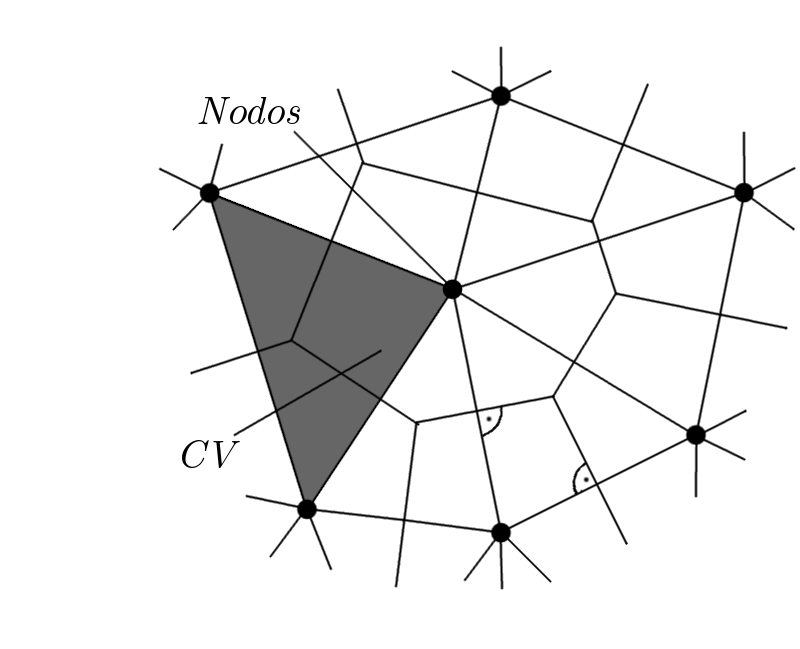
\includegraphics[width=8cm]{Img/4-32}
	\caption{Centroide por la intersección de las Bisetrices}
	\label{img:4-32}
\end{figure}
Finalmente para casos tridimensionales se utilizan las mismas técnicas bidimensionales utilizando hexaedros y tetraedros como los VC.

Una vez definido el VC, la ecuación de balance que describe el problema es formulada de manera integral para cada VC. Integrando la ecuación \ref{eq:4-1} sobre un VC arbitrario y aplicando el teorema de la divergencia, obetenemos:
\begin{equation}
	\int_S \left( \rho v_i \phi - \alpha \frac{\partial \phi}{\partial x_i} \right)n_i DS = \int_V f dV ~,
	\label{eq:4-2}
\end{equation}
donde $S$ es la superficie del VC y $n_i$ es la normal de la superficie. 

Por ejemplo, si consideramos los VC como cuadriláteros usando el enfoque en la celda y la notación representada en la figura \ref{img:4-4}, para distinguir los puntos (centroides, centro de las caras y vértices del VC) y los vectores normales a la superficie.
\begin{figure}[h!]
	\centering
	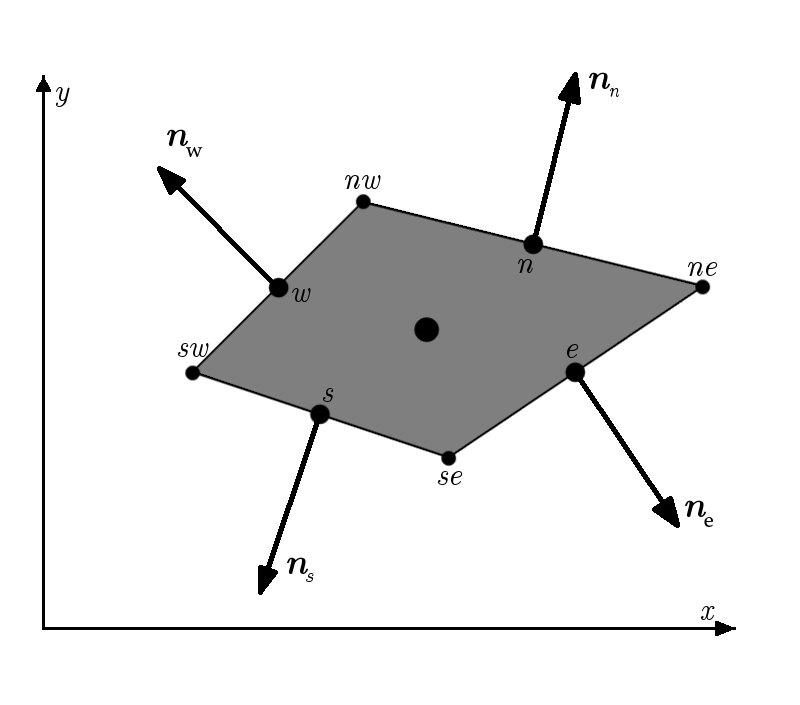
\includegraphics[width=8cm]{Img/4-5}
	\caption{Normales y nodos centrales de cada arista}
	\label{img:4-4}
\end{figure}

La integral de superficie en \ref{eq:4-2} puede ser dividida en cuatro integrales sobre las caras $S_c (c=e,w,n,s)$ del VC, obteniendo:
\begin{equation}
	\sum_c \int_{S_c} \left( \rho v_i \phi - \alpha \frac{\partial \phi}{\partial x_i} \right) n_{ci} dS_c = \int_V f dV.
	\label{eq:4-3}
\end{equation}

La ecuación \ref{eq:4-3} representa el balance de los flujos convectivos ($F_c^C$) y difusivos ($F_c^D$) a través de las caras ($c$) del VC, con
\begin{equation}
	F^C_c = \int_{S_c} \left( \rho v_i \phi \right) n_{ci} d S_c ~~~ y ~~~ F^D_c = - \int_{S_c} \left( \alpha \frac{\partial \phi}{\partial x_i} \right) n_{ci} d S_c . \nonumber
\end{equation}

Para la cara $S_e$, la normal $n_e = (n_{e1},n_{e2})$ es definida con las siguientes condiciones:
\begin{equation}
	\left( x_{ne} - x_{se} \right) \dot n_e = 0 ~~~ y ~~~ \vert n_e \vert = 1. \nonumber
\end{equation}

Los vecinos que comparten una cara, el flujo total $F_c = F_c^C + F_c^D$ a través de dicha cara es igual pero con el signo opuesto. Si nos concentramos en el VC alrededor del punto $P$ (Figura \ref{img:4-5}), el flujo $F_e$ es igual al flujo $-F_w$ del VC del punto $E$ ($(n_e)_P = -(n_w)_E$). De esta manera se evita calcular dos veces los flujos y se asegura que los flujos son iguales (\textit{conservación}).
\begin{figure}[h!]
	\centering
	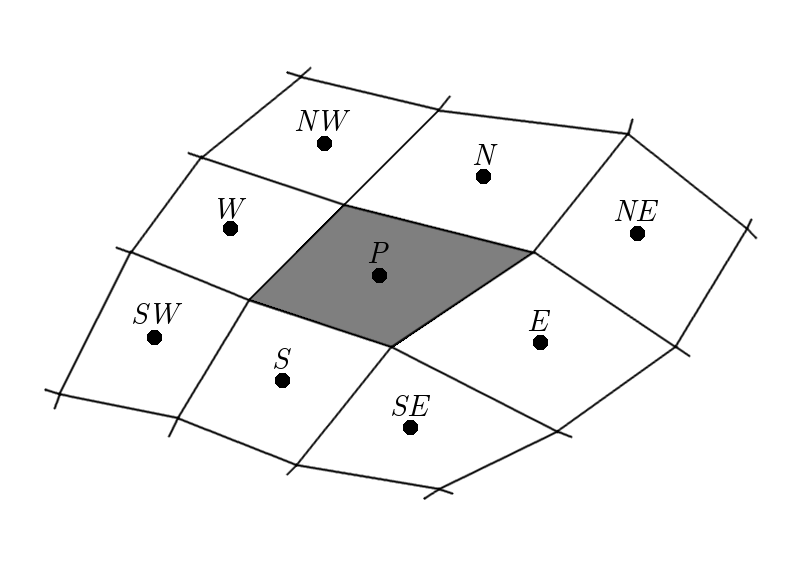
\includegraphics[width=8cm]{Img/4-6}
	\caption{Vecinos del volumen de control P}
	\label{img:4-5}
\end{figure}

\section{Aproximación de las integrales de superficie y volumen}

Para aproximar las integrales de superficie en \ref{eq:4-3}, planteamos un caso general:
\begin{equation}
	\int_{S_e} w_i n_{ei} dS_e \nonumber
\end{equation} 
donde $w = (w_1(x) , w_2(x))$ es una función general que se integra sobre la cara $S_e$ del VC. Para aproximar la integral se puede utilizar diversos enfoques involucrando uno o más valores de la cara del VC a integrar. La aproximación más sencilla es de utilizar el punto médio de la cara para obtener:
\begin{equation}
	\int_{S_e} w_i n_{ei} dS_e \approx g_e \delta S_e
	\label{eq:4-5}
\end{equation}
donde $g_e = w_{ei} n_{ei}$ es la componente normal de $w$ en la cara $e$. La aproximación obtenida en \ref{eq:4-5} corresponde a la \textit{regla del punto medio}, la cual tiene un orden de aproximación de 2do orden.

Podemos mencionar otros enfoques que utilizan más puntos en la cara del VC, tales como la \textit{regla del trapezoide} que utiliza los dos puntos extremos ($(g_{ne} + g_{se})/2$) con un 2do orden de aproximación; y la \textit{regla de Simpson} que agrega el punto central ($(g_{ne} + 4g_{e} + g_{se})/6$) para mejorar la aproximación a 4to orden. Cabe aclarar que el orden de los métodos depende de $\delta S_e$, es decir, para la regla del punto medio el error se estima como:
\begin{equation}
	\frac{\delta S_e^2 M}{2}  \nonumber
\end{equation}
donde $M$ es la cota superior para $w'(x)$, es decir, $\vert w'(x) \vert \leq M ~~ \forall x$.

Aplicando la regla del punto medio para aproximar las integrales en los flujos convectivos y difusivos de las caras del VC en \ref{eq:4-3}, obtenemos:
\begin{equation}
	F_c^C \approx \rho v_i n_{ci} \delta S_c \phi_c ~~~ y ~~~ F_c^D \approx - \alpha n_{ci} \delta S_c \left( \frac{\partial \phi}{\partial x_i} \right)_c , \nonumber
\end{equation}
donde por simplicidad asumimos que $\rho, ~ v_i,$ y $\alpha$ son constantes en toda la cara del VC.

%Para aproximar la integral en el término fuente asumimos que $f_p$ es el valor de $f$ en el centro del VC por lo tanto aplicando la regla del punto medio obtenemos:
\begin{equation}
	\int_V f dV \approx f_P \delta V, \nonumber
\end{equation} 
donde $\delta V$ es el volumen en el VC, el cual para elementos cuadriláteros está dado por:
\begin{equation}
	\delta V = \frac12 \vert(x_{se} - x_{nw})(y_{ne} - y_{sw})-(x_{ne} - x_{sw})(y_{se} - y_{nw})\vert \nonumber .
\end{equation}

Para mallas cartesianas bidimensionales, el error que introduce la aproximación depende del volumen ($\delta V$). Una aproximación alternativa es utilizar la regla de simpson, la cual establece:
\begin{equation}
	\int_v f dV \approx \frac{\delta V}{36}(16f_p + 4f_e + 4f_w + 4f_n + 4f_s + f_{ne}+ f_{se}+ f_{nw}+ f_{sw}). \nonumber
\end{equation}

Cabe destacar que para los casos tridimensionales las integrales de volumen bidimensionales pueden extenderse de manera análoga.

Resumiendo, aplicando la regla del punto medio obtenemos la siguiente ecuación de balance (\ref{eq:4-3}):
\begin{equation}
	\underbrace{\sum_c \rho v_i n_{ci} \delta S_c \phi_c}_{flujo ~ conv.} - \underbrace{\sum_c \alpha n_{ci} \delta S_c \left( \frac{\partial \phi}{\partial x_i} \right)_c}_{flujo ~ dif.} = \underbrace{f_P \delta V}_{fuente}.
	\label{eq:4-6}
\end{equation}

Una vez aproximadas las integrales, debemos obtener los valores de $\phi$ y su derivada en las caras del VC para los flujos convectivos y difusivos respectivamente, utilizando los valores en los nodos (centroides). Para facilitar la comprensión utilizaremos mallas cartesianas en dos dimensiones como muestra la figura \ref{img:4-8} en donde encontramos la partidularidad de:
\begin{equation}
	n_e = e_1, ~~ n_w = -e_1, ~~ n_n = e_2, ~~ n_s = -e_2
\end{equation}
\begin{figure}[h!]
	\centering
	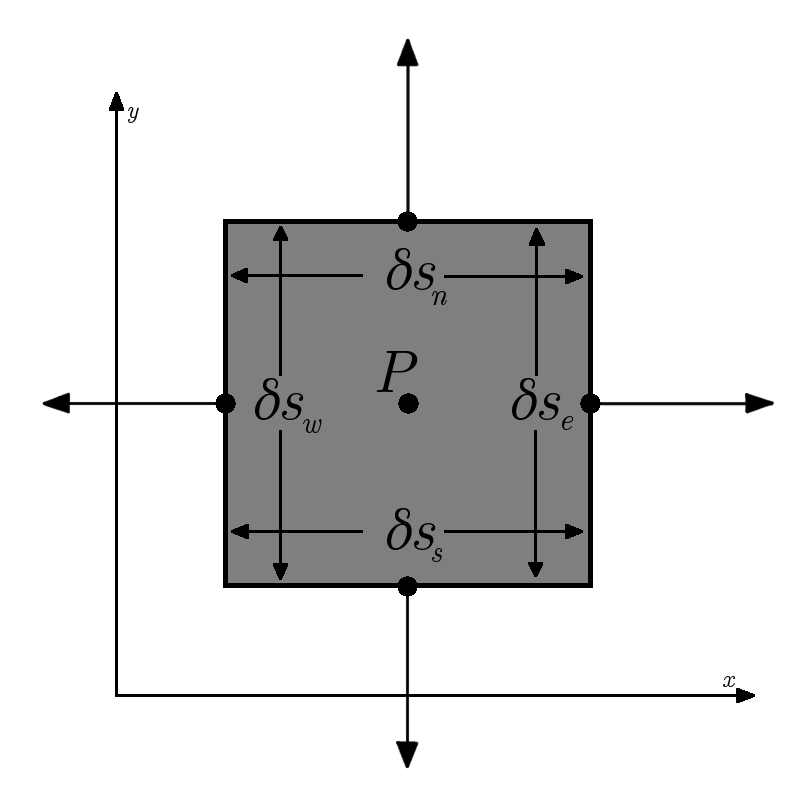
\includegraphics[width=8cm]{Img/4-8}
	\caption{Elemento cartesiano}
	\label{img:4-8}
\end{figure}

\pagebreak

\section{Discretización del término convectivo}

Para aproximar el flujo convectivo $F_c^C$ en la cara $c$, es necesario aproximar $\phi_c$ utilizando los valores de los centroides del VC y sus respectivos vecinos. Existen diversas maneras para obtener $\phi_c$ (\textit{técnicas de interpolación}), los cuales serán explicados a continuación para casos unidimensionales considerando la cada $S_e$, ya que su extensión a dos o tres dimensiones se puede tratar de manera análoga.

\subsection{Esquema de diferencia centradas}

El \textit{esquema de diferencia centradas} (EDC) aproxima $\phi_e$ utilizando una interpolación lineal con los valores de la vecindad de $P$ y $E$ (Figura \ref{img:4-9}):
\begin{equation}
	\phi_e \approx \gamma_e \phi_E + (1-\gamma_e) \phi_P
	\label{eq:4-7}
\end{equation}
El factor de interpolación $\gamma_e$ se define como:
\begin{equation}
	\gamma_e = \frac{x_e - x_P}{x_E - x_P}. \nonumber
\end{equation}

La aproximación \ref{eq:4-7} tiene una aproximación de 2do orden para cualquier tipo de malla, es decir, para las estructuradas como las no-estructuradas. 
\begin{figure}[h!]
	\centering
	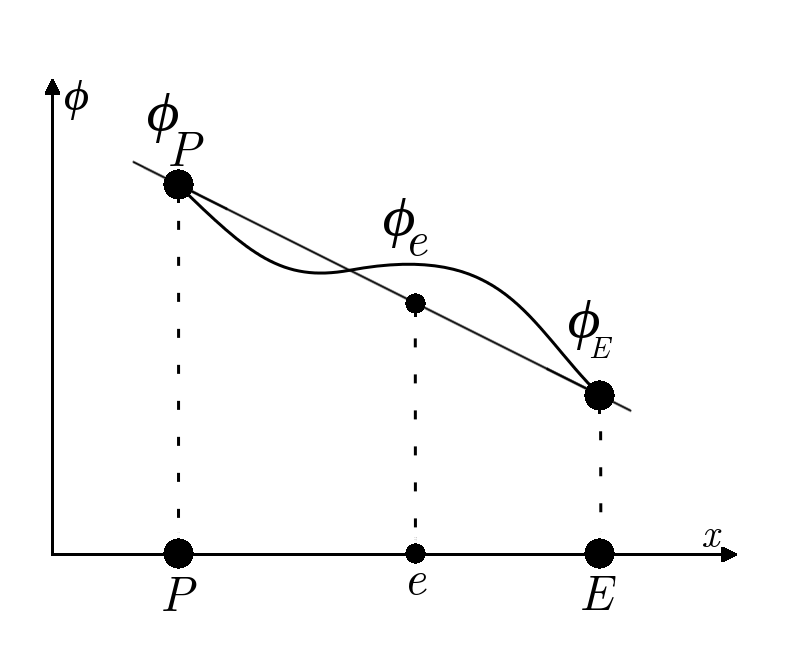
\includegraphics[width=8cm]{Img/4-9}
	\caption{Interpolación centrada}
	\label{img:4-9}
\end{figure}
Esto se puede demostrar expandiendo la serie de Taylor para $\phi$ alrededor del punto $x_P$:
\begin{equation}
	\phi(x) = \phi_P + (x-x_P) \left( \frac{\partial \phi}{\partial x} \right)_P + \frac{(x-x_P)^2}{2} \left( \frac{\partial^2 \phi}{\partial x^2} \right)_P + T_H, \nonumber
\end{equation}
donde $T_H$ denota el término de mayor orden. Evaluando esta serie en los puntos $x_e$, $x_E$ y aplicando la diferencia obtenemos:
\begin{equation}
	\phi(x) = \gamma_e \phi_E + (1-\gamma_e)\phi_P + \frac{(x_e-x_P)(x_E-x_e)}{2} \left( \frac{\partial^2 \phi}{\partial x^2} \right)_P + T_H, \nonumber
\end{equation}
la cual demuestra que el error depende cuadráticamente de la discretización espacial.

Al agregar puntos en la interpolación del esquema de diferencias centradas, obtenemos una aproximación de mayor orden. Por ejemplo, para un 4to orden en una malla equidistante obtenemos:
\begin{equation}
	\phi_3 = \frac{1}{48}(-3\phi_{EE} + 27\phi_3 + 27\phi_P -3\phi_W), \nonumber
\end{equation}
donde $EE$ denota el ``este" $~$ del vecino E (ver figura 4.11). Cabe aclarar que el uso de esta formula solo toma sentido si es utilizada en conjunto con una discretización integral de 4to orden, como la regla de Simpson. Solamente para ese caso, la aproximación total del flujo convectivo es de 4to orden.

Como desventaja, la aproximación de diferencias centradas puede generar oscilaciones en la solución numérica que no representan la física del problema.

\subsection{Técnicas UPWIND}

La principal idea de las técnicas \textit{UPWIND} es hacer la interpolación teniendo en cuenta la dirección de la velocidad (Figura \ref{img:4-10}).
\begin{figure}[h!]
	\centering
	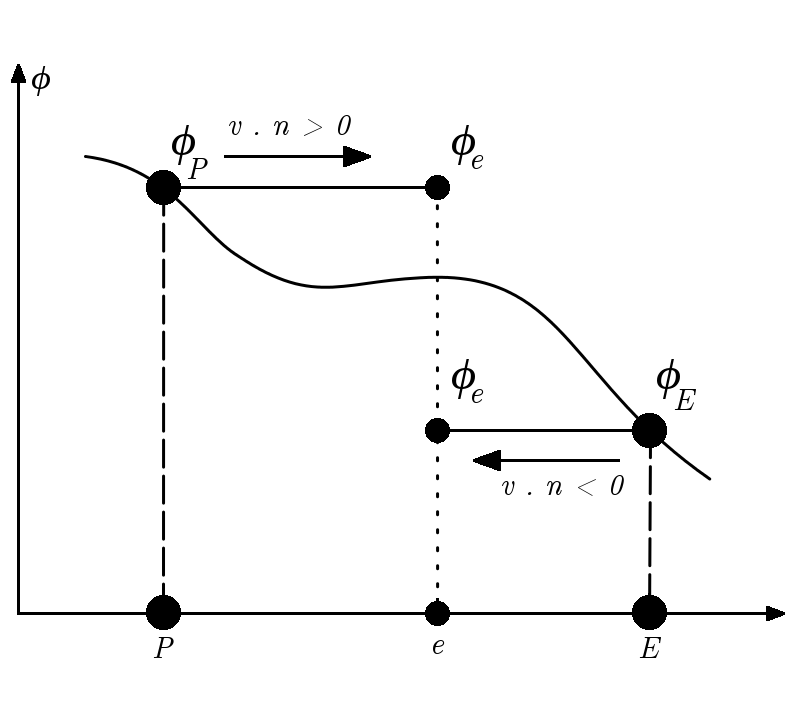
\includegraphics[width=8cm]{Img/4-10}
	\caption{Interpolación upwind}
	\label{img:4-10}
\end{figure}
La técnica más sencilla resulta de aproximar $\phi$ utilizando una función dependiente de la dirección del flujo de masa:
\begin{eqnarray}
	\phi_e = \phi_P, & si \ v_e \cdot n_e > 0, \nonumber \\ 
	\phi_e = \phi_E, & si \ v_e \cdot n_e < 0. \nonumber
\end{eqnarray}
Este método es llamado \textit{esquema de diferencias upwind} (EDU). La expansión en series de Taylor para $\phi$ alrededor del punto $x_P$, evaluado en el punto $\phi_e$ obtenemos:
\begin{equation}
	\phi_e = \phi_P + (x_e-x_P) \left( \frac{\partial \phi}{\partial x} \right)_P + \frac{(x_e-x_P)^2}{2} \left( \frac{\partial^2 \phi}{\partial x^2} \right)_P + T_H. \nonumber
\end{equation}
esto muestra que el EDU independiente del tipo de grilla, su error es de 1er orden. Entonces el error introducido por la aproximación del flujo convectivo $F^c_e$ es
\begin{equation}
	\rho_e v_e \cdot n_e dS_e (x_e -x_P) \left( \frac{\partial \phi}{\partial x} \right)_P. \nonumber
\end{equation}
Esta desventaja en el bajo orden de aproximación se fortalece al asegurar la convergencia del algoritmo, evitando las oscilaciones que generaba el EDC de 2do orden. 

Para solventar la problemática en el orden de aproximación, surge utilizar más valores en la interpolación (Figura \ref{img:4-11}). En la literatura se conoce como \textit{interpolación cuadrática UPWIND para cinemática convectiva (QUICK)}, el cual utiliza la vecindad $P$, $E$ y un tercer punto: $W$ o $EE$ dependiendo de la dirección del flujo. 
\begin{figure}[h!]
	\centering
	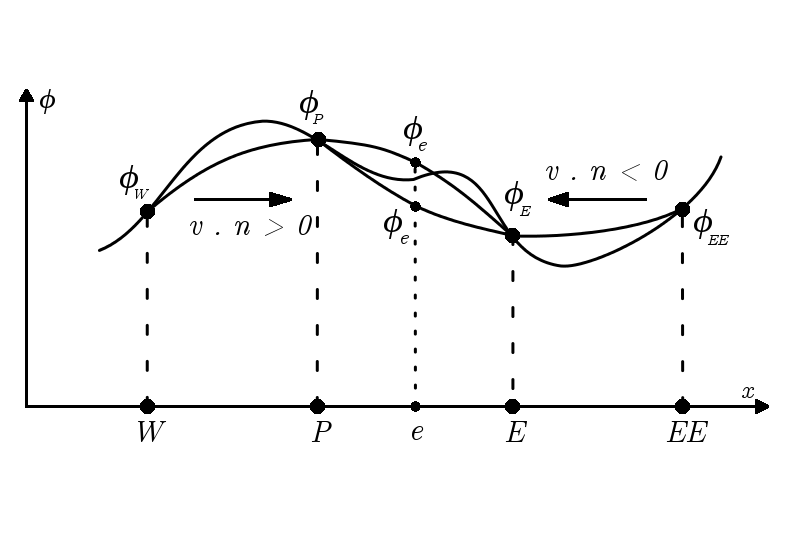
\includegraphics[width=8cm]{Img/4-11}
	\caption{Interpolación quick}
	\label{img:4-11}
\end{figure}

La aproximación QUICK se define:
\begin{eqnarray}
	\phi_e = a_1 \phi_E - a_2 \phi_W + (1 - a_1 + a_2)\phi_P, & si \ v_e \cdot n_e > 0, \nonumber \\
	\phi_e = a_1 \phi_E - a_2 \phi_W + (1 - a_1 + a_2)\phi_P, & si \ v_e \cdot n_e > 0, \nonumber
\end{eqnarray}
donde
\begin{eqnarray}
	a_1 = \frac{(2-\gamma_w)\gamma_e^2}{1+\gamma_e -\gamma_w}, & & a_2 = \frac{(1-\gamma_e)(1-\gamma_w)^2}{1+\gamma_e-\gamma_w}, \nonumber \\
	b_1 = \frac{(1+\gamma_w)(1-\gamma_e)^2}{1+\gamma_{ee} - \gamma_e}, & & b_2 = \frac{\gamma_{ee}^2 \gamma_e}{1+\gamma_{ee}-\gamma_e}. \nonumber
\end{eqnarray}
Para grillas equidistantes ($dx = cte \ y \ dy = cte$) tenemos:
\begin{equation}
	a_1 = \frac{3}{8}, \ \ a_2 = \frac{1}{8}, \ \ b_1 = \frac{3}{8}, \ \ b_2 = \frac{1}{8}. \nonumber
\end{equation}
En este caso la interpolación QUICK tiene una aproximación de 3er orden. Sin embargo, si lo utilizamos con una integración numérica de 2do orden, la aproximación del flujo convectivo será de 2do orden, pero tiene más presición que el esquema CDS.

\section{Discretización del flujo difusivo}

Para discretizar el flujo difusivo es necesario obtener una aproximación a la componente normal de la derivada de $\phi$ en la cara del VC. Continuando con el enfoque anterior, utilizaremos la cara este $S_e$ del VC. Una primera aproximación para mallas cartesianas es utilizar el enfoque de diferencias finitas para la primera derivada. La discretización más simple es aplicar el esquema de diferencia centrada
\begin{equation}
	\left( \frac{\partial \phi}{\partial x} \right)_e \approx \frac{\phi_E - \phi_P}{x_E - x_P},
	\label{eq:4.9}
\end{equation}
la cual asume que $\phi$ es una función lineal entre los puntos $x_E$ y $x_P$ (Figura \ref{img:4-12}). Para la evaluar el error de esta aproximación, realizamos una expansión de la serie de Taylor alrededor del punto $x_e$ hacia los nodos $x_P$ y $x_E$:
\begin{eqnarray}
	\left( \frac{\partial \phi}{\partial x} \right)_e =  \frac{\phi_E - \phi_P}{x_E - x_P} + \frac{(x_e - x_P)^2-(x_E -x_e)^2}{2(x_E -x_P)} \left( \frac{\partial^2 \phi}{\partial x^2} \right)_e \nonumber \\ 
	- \frac{(x_e - x_P)^3-(x_E -x_e)^3}{6(x_E -x_P)} \left( \frac{\partial^3 \phi}{\partial x^3} \right)_e + T_H
\end{eqnarray}

Podemos observar que para una malla equidistante el error es de 2do orden, ya que en este caso el coeficiente de la segunda derivada es cero. 
\begin{figure}[h!]
	\centering
	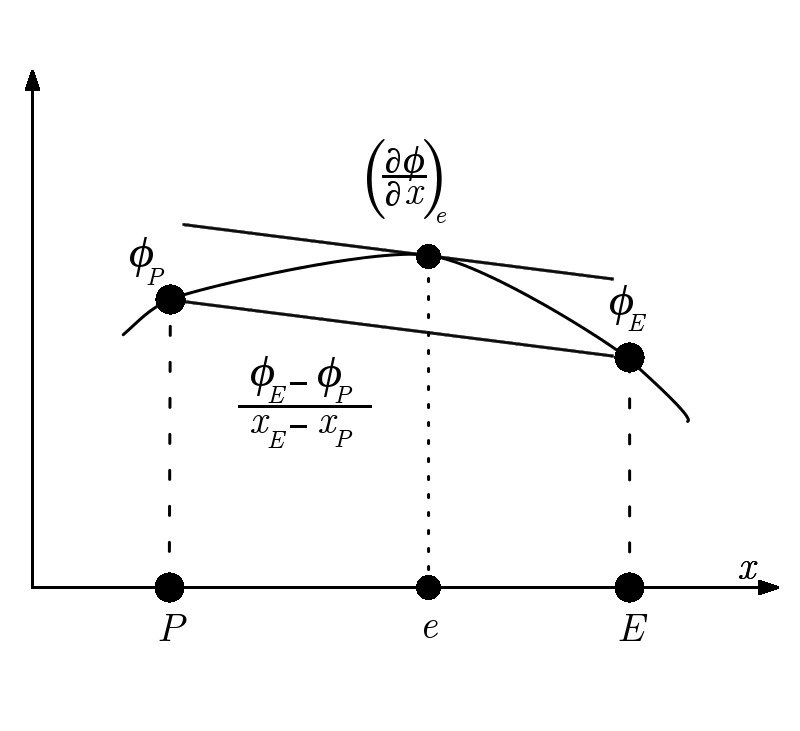
\includegraphics[width=8cm]{Img/4-12}
	\caption{Esquema de diferencias centradas}
	\label{img:4-12}
\end{figure}
Para el caso contrario, mallas no-equidistantes obtenemos una nueva disposición del error, el cual es proporcional al refinamiento de la grilla en ambos sentidos:
\begin{equation}
	\frac{(1-\epsilon_e)(x_e - x_P)}{2} \left( \frac{\partial^2 \phi}{\partial x^2} \right)_e \ \ \epsilon_e = \frac{x_e - x_e}{x_e - x_P}.
\end{equation}
Esto quiere decir que el error es de 1er orden y puede aumentarse si $\epsilon$ no tiende a valer 1, este aspecto hay que tenerlo en cuenta cuando se genera la malla, es decir, evitar que halla mucha diferencia en las dimensiones de las vecindades.

Una aproximación de 4to orden puede ser obtenido en para mallas equidistantes por
\begin{equation}
	\left( \frac{\partial \phi}{\partial x} \right)_e \approx \frac{1}{24 \Delta x} (\phi_W - 27\phi_P + 27\phi_E - \phi_{EE}),
\end{equation}
la cual puede ser utilizada en conjunto con la regla de simpson para obtener una aproximación de 4to orden para el flujo difusivo.

\section{Tratamiento del contorno}

A modo de simplificar la explicación tendremos en cuenta dos tipos de condiciones de contorno, las de valor impuesto y las de flujo impuesto, las cuales son las más utilizadas considerando el tipo de problemas que se resolverán. Además continuamos utilizando la ecuación de transporte escalar con una malla cartesiana enfocándonos en la cara oeste del VC como lo muestra la figura \ref{img:4-13}.

Comenzamos para el caso del valor impuesto, es decir $\phi_w = \phi^0$. Para el flujo convectivo en el contorno es aproximado:
\begin{equation}
	F_w^C \approx \rho v_e \cdot n_e dS_e \phi_w = \rho v_e \cdot n_e dS_e \phi^0.
\end{equation}

Con esta aproximación el flujo convectivo $F_w^C$ es conocido, por lo tanto se introduce en el término fuente de la ecuación de balance (\ref{eq:4-6}). 

El flujo difusivo sobre el contorno es determinado de la misma manera que para una cara del interior del dominio. De manera análoga como la ecuación (4.9), la derivada en el contorno se puede aproximar:
\begin{equation}
	\left( \frac{\partial \phi}{\partial x} \right)_w \approx \frac{\phi_P - \phi_w}{x_p - x_w} = \frac{\phi_P - \phi^0}{x_P -x_w}.
\end{equation}
La cual corresponde a una discretización hacia delante de la primera derivada, la cual es de 1er orden. Cabe aclarar que se pueden utilizar aproximaciones con mejor presición, pero mientras que la distancia entre el contorno $w$ y el punto $P$ sea menor a la distancia entre dos puntos vecinos en el interior del dominio (la mitad para una grilla equidistante), una baja aproximación en el contorno no afecta en la precisión.
\begin{figure}[h!]
	\centering
	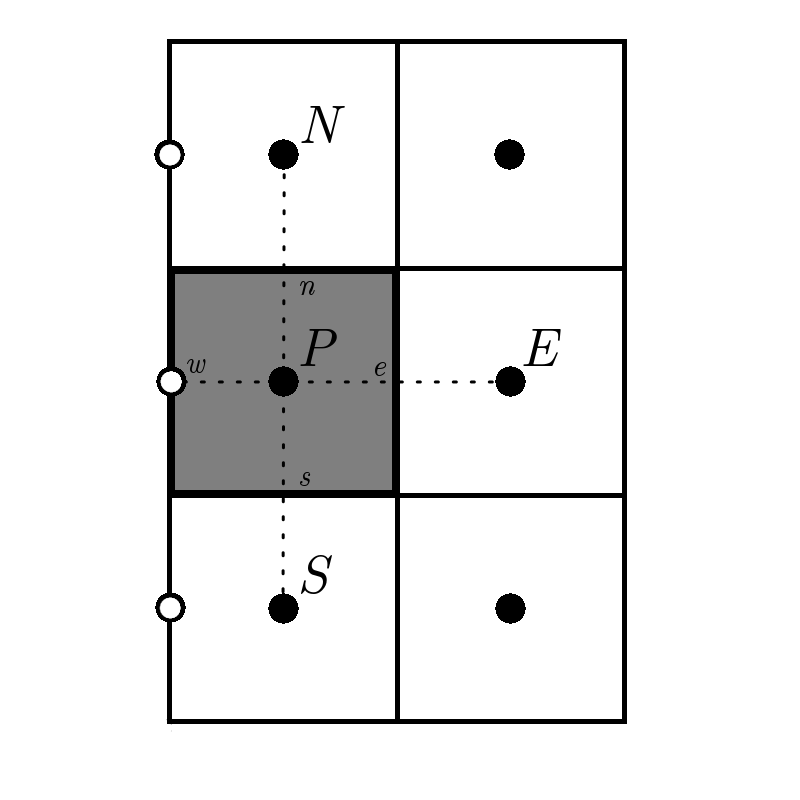
\includegraphics[width=8cm]{Img/4-13}
	\caption{Contorno en la cara oeste}
	\label{img:4-13}
\end{figure}

Ahora consideremos el caso del flujo impuesto $F_w = F^0$ en la cara oeste. Para el flujo convectivo podemos aproximar el valor en el contorno utilizando la primera derivada:
\begin{equation}
	F^0 \approx \frac{\phi_w - \phi_P}{x_w - x_P} ~ , ~ \phi_w \approx F^0 (x_w - x_P) + \phi_P \nonumber
\end{equation} 
De esta manera el término convectivo en la cara $w$ queda determinado por
\begin{equation}
	\rho v_e \cdot n_e dS_e [F^0 (x_w - x_P) + \phi_P], \nonumber
\end{equation}
el cual se divide en dos término, el primero aporta al término fuente y el segundo al nodo $P$. 

El flujo difusivo ya está impuesto por lo tanto
\begin{equation}
	\left(\frac{\partial \phi}{\partial x} \right)_w = F^0, \nonumber
\end{equation}
dado que el flujo difusivo es conocido se introduce en el término fuente.

\chapter{Discretización temporal}

Muchas aplicaciones prácticas tienen procesos que se consideran no estacionarios y por lo tanto requieren una simulación numérica utilizando un modelo que dependa del tiempo. El tiempo tiene un rol importante en las ecuaciones diferenciales porque, a diferencia de la discretización espacial, hay una dirección a tomar debido al principio de la causalidad. Este hecho debe ser tomado en cuenta por las técnicas de discretización. En este capítulo se analizarán los aspectos más importantes sobre el tema.

\section{Temas básicos}

Para los problemas físicos no estacionarios que dependen del paso de tiempo, consideraremos dos principales tipo de dependencia: transporte y vibración. Los vórtices generados por un fluido que fluye a través de objetos (figura \ref{img:5-1}) 
\begin{figure}[h!]
	\centering
	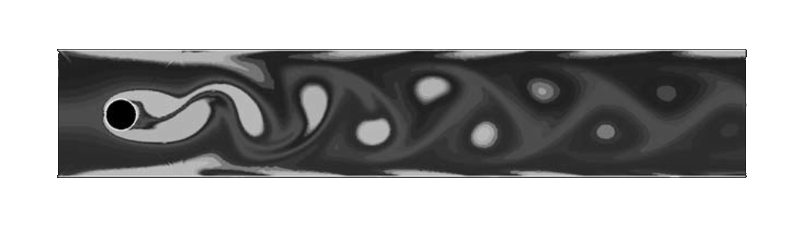
\includegraphics[width=8cm]{Img/5-1}
	\caption{Vórtice de Kárman}
	\label{img:5-1}
\end{figure}
o la vibración de una estructura (figura \ref{img:5-2}), son claros ejemplos.
\begin{figure}[h!]
	\centering
	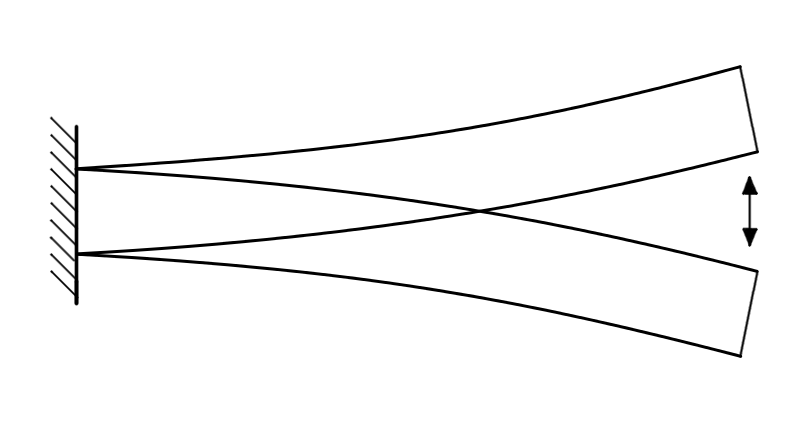
\includegraphics[width=8cm]{Img/5-2}
	\caption{Vibración de una viga}
	\label{img:5-2}
\end{figure}

Mientras que la ecuación de transporte no-estacionario solo utiliza la primera derivada respecto del tiempo, las que representan el proceso de vibración tiene una derivada de segundo orden. Problemas denominados \textit{parabólicos} e \textit{hiperbólicos} respectivamente.
Un ejemplo de problema parabólico es la ecuación general de transporte escalar no-estacionario,
\begin{equation}
	\frac{\partial (\rho \phi)}{\partial t} + \frac{\partial}{\partial x_i} \left( \rho v_i \phi - \alpha \frac{\partial \phi}{\partial x_i} \right) = f
	\label{eq:5-1}
\end{equation}
Un problema del tipo hiperbólico es la ecuación de elasticidad no-estacionaria
\begin{equation}
	\rho A \frac{\partial^2 w}{\partial t^2} + \frac{\partial^2}{\partial x^2} \left( B \frac{\partial^2 w}{\partial x^2} \right) + f_q = 0
	\label{eq:5-2}
\end{equation}
En comparación con los problemas estacionarios, el tiempo es una nueva coordenada independiente ($\phi(\textbf{x}, t$). Para poder resolver problemas no-estacionarios, es necesario partir de una condición inicial además de las condiciones de contorno (que también pueden depender del tiempo). Para problemas de transporte (\ref{eq:5-1}):
\begin{equation}
	\phi(\textbf{x},t_0) = \phi^0(\textbf{x}), \nonumber
\end{equation}
mientras que para problemas de vibración (\ref{eq:5-2}):
\begin{equation}
	w(\textbf{x},t_0) = w^0(\textbf{x}) \ \ y \ \ \frac{\partial w}{\partial t}(\textbf{x},t_0) = w^1(\textbf{x}). \nonumber
\end{equation}
Para resolver problemas no-estacionarios se discretiza el dominio espacial con cualquier tipo de procedimiento, para obtener un sistema de ecuaciones diferenciales para cada nodo del tipo $\phi(\textbf{x},t)$. Discretizando \ref{eq:5-1} utilizando el MVF para cada volumen de control obtenemos:
\begin{equation}
	\frac{\partial \phi_P}{\partial t} = \frac{1}{\rho \delta V} \left[ -a_P(t) \phi_P + \sum_c a_c(t)\phi_c + b_P(t) \right],
	\label{eq:5-3}
\end{equation}
donde, por simplicidad asumimos que la densidad $\rho$ y el volumen $\delta V$ son constantes.
Primero discretizamos el intervalo de tiempo $[t_0,T]$ en sub-intevalos $\Delta t$ donde:
\begin{equation}
	t_{n+1} = t_n + \Delta t = t_0 + n\Delta t, ~ n=0,1,2 ... \nonumber
\end{equation}

El principio de causalidad establece que la solución en el tiempo $t_{b+1}$ solamente puede depender a pasos de tiempo \textit{anteriores} ($t_n, t_{n-1}, ...$). En este sentido el tiempo es una coordenada en ``una dirección", es decir, que la discretización temporal consiste en una extrapolación. Comenzando a partir de las condiciones iniciales, las variables desconocidas $\phi$ son sucesivamente calculadas en los puntos $t_1,t_2,...$ (figura \ref{img:5-3}).
\begin{figure}[h!]
	\centering
	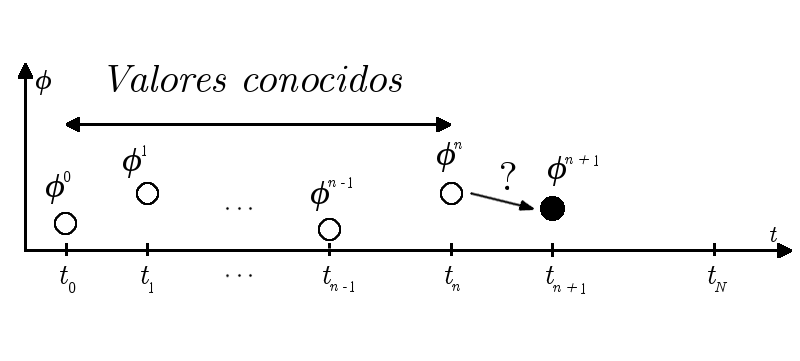
\includegraphics[width=8cm]{Img/5-3}
	\caption{Paso de tiempo}
	\label{img:5-3}
\end{figure}

Teniendo en cuenta la cantidad de pasos anteriores que se utilizan para obtener la nueva solución en $t_{n+1}$, el método se clasifica en los métodos de un paso y los multi-pasos. Los primeros calculan el paso $t_{n+1}$ utilizando solamente el instante anterior $t_n$, en cambio, los segundos tienen en memoria más instantes de tiempo ($t_n, t_{n-1},\cdots$) para calcular el instante siguiente. Otra clasificación y de mayor importancia, consiste en diferenciar los métodos en dos categorías dependiendo de la elección de puntos en el tiempo:
\begin{itemize}
	\item[$\bullet$]  \textit{Métodos Explícitos}: discretización que consiste en utilizar estados previos para calcular el nuevo instante,
	\begin{equation}
		\phi_{n+1} = F(\phi^n,\phi^{n-1},...). \nonumber
	\end{equation}
	\item[$\bullet$] \textit{Métodos Implícitos}: en este caso también utiliza el instante a calcular además de los anteriores,
	\begin{equation}
		\phi_{n+1} = F(\phi^{n+1},\phi^n,\phi^{n-1},...). \nonumber
	\end{equation}
\end{itemize}

La distinción entre los métodos implícitos y explícitos es muy importante ya que tienen diferentes atributos o características en los esquemas numéricos que resuelven el sistema.

\section{Métodos Explícitos}

Comenzamos con el ejemplo más sencillos para la discretización temporal, el \textit{método explícito de Euler}, el cual obtiene una aproximación temporal derivando el tiempo con un esquema diferencial hacia delante:
\begin{equation}
	\frac{\partial \phi}{\partial t}(t_n) \approx \frac{\phi^{n+1} - \phi^n}{\Delta t_n} = F(\phi^n).
	\label{eq:5-4}
\end{equation}
La cual corresponde a una aproximación de la derivada temporal utilizando las componentes $\phi_i$ en el tiempo $t_n$ utilizando la pendiente de la recta que une los puntos $\phi_i^n$ y $\phi_i^{n+1}$ (Figura \ref{img:5-5}). Este método es de primer orden de aproximación respecto del tiempo.
\begin{figure}[h!]
	\centering
	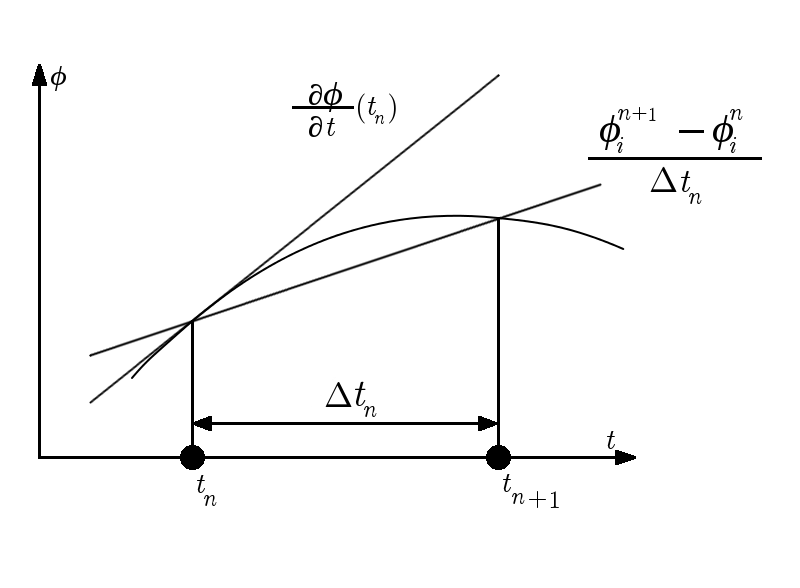
\includegraphics[width=8cm]{Img/5-5}
	\caption{Aproximación de Euler hacia delante}
	\label{img:5-5}
\end{figure}

La relación \ref{eq:5-4} puede ser resuelta explícitamente para $\phi^{n+1}$:
\begin{equation}
	\phi^{n+1} = \phi^n + \Delta t_n F(\phi^n). \nonumber
\end{equation}
El término derecho contiene solamente valores de tiempo conocidos, de manera tal que la ecuación para los valores en el tiempo $t_{n+a}$ en los diferentes puntos de la grilla están desacoplados, por lo tanto pueden ser calculado de manera independiente entre ellos. Esta es una característica de los métodos explícitos.

Consideremos como ejemplo el caso unidimensional no-estacionario puramente difusivo con parámetros del material constante:
\begin{equation}
	\frac{\partial \phi}{\partial t} = \frac{\alpha }{\rho} \frac{\partial^2 \phi}{\partial x^2}.
	\label{eq:5-5}
\end{equation}
Utilizando el MVF como discretización espacial con un esquema diferencial centrado para el término difusivo para una malla equidistante con un $\delta x$ para cada VC, la ecuación diferencial queda:
\begin{equation}
	\frac{\partial \phi_P}{\partial t}(t) \Delta x = \frac{\alpha}{\rho} \frac{\phi_E(t) - \phi_P(t)}{\Delta x} - \frac{\alpha}{\rho} \frac{\phi_P (t) - \phi_W(t)}{\Delta x}
	\label{eq:5-6}
\end{equation}
El método explícito de Euler con un paso de tiempo $\Delta t$ dado, obtenemos la siguiente aproximación:
\begin{equation}
	\frac{\phi_P^{n+1} - \phi_P^n}{\Delta t} \Delta x= \frac{\alpha}{\rho} \frac{\phi_E^n - \phi_P^n}{\Delta x} - \frac{\alpha}{\rho} \frac{\phi_P^n - \phi_W^n}{\Delta x}. \nonumber
\end{equation}
Despejando $\phi_P^{n+1}$:
\begin{equation}
	\phi_P^{n+1} = \frac{\alpha \Delta t}{\rho \Delta x^2}(\phi_E^n + \phi_W^n) + \left( 1- \frac{2 \alpha \Delta t}{ \rho \Delta x^2} \right) \phi_P^n. \nonumber
\end{equation}
Una observación interesante es que se necesita un número de pasos hasta que las condiciones de contorno afecten en interior del dominio. Con una malla más refinada, más pasos son requeridos para que el contorno influya en el interior aunque se utilice el mismo paso de tiempo. Esta relación entre el paso de tiempo y la resolución espacial está limitada a condiciones de estabilidad, las cuales definen dos números de estabilidad a considerar:
\begin{equation}
	D = \frac{\alpha \Delta t}{\rho \Delta x^2} ~~ , ~~ C = \frac{v \Delta t}{\Delta x}, \nonumber
\end{equation}
donde $D$ es el \textit{número de difusión} y C es el \textit{número de Courant}, los cuales restringen el paso de tiempo para casos de transporte difusivos y convectivos respectivamente. Por ejemplo, consideramos la ecuación de transporte de la propiedad $\phi$ utilizando un esquema $UPWIND$ de primer orden para el término convectivo, un esquema de diferencias centradas para el campo difusivo y reorganizando obtenemos:
\begin{equation}
	\phi^{n+1}_P = D\phi_E^n + (D + C) \phi_W^n + (1-2D-C)\phi_P^n, \nonumber
\end{equation}
donde las variablas $D$ y $C$ son las componente difusivas y convectivas respectivamente. El sistema tiene que cumplir con la siguiente restricción para asegurar la estabilidad:
\begin{equation}
	\Delta t < \frac{\rho \Delta x^2}{2\alpha + \rho v \Delta x}. \nonumber
\end{equation}
El cual tiene en cuenta los términos difusivos y conevectivos.

Otra alternativa en la discretización temporal explícita de un paso es el \textit{método explísito de Euler modificado} introducido por \textit{Collatz (1960)}, el cual es de segundo orden para mallas equidistantes y se define como:
\begin{equation}
	\frac{\phi^{n+1} - \phi^n}{\Delta t_n} = F\left( \phi^n + \frac{\Delta t_n}{2} F(\phi^n) \right). \nonumber
\end{equation}

Los métodos explícitos de un paso de \textit{Runge-Kutta} son frecuentemente utilizados en fluidos aerodinámicos. Un ejemplo de 4to orden:
\begin{equation}
	\frac{\phi^{n+1} - \phi^n}{\Delta t_n} = \frac16 (f_1 + 2f_2 + 2f_3 + f_4), \nonumber
\end{equation}
donde,
\begin{eqnarray}
	f_1 = F(\phi^n), & ~ & f_2 = F \left( \phi^n + \frac{\Delta t_n}{2} f_1 \right), \nonumber \\
	f_3 = F \left( \phi^n + \frac{\Delta t_n}{2} f_2 \right), & ~ & f_4 = F \left( \phi^n + \Delta t_n f_3 \right). \nonumber
\end{eqnarray}

Los métodos multi-pasos utilizan dos o más pasos de tiempo para aproximar la derivada temporal, pero siempre deben comenzar con un método de un paso, porque las condiciones iniciales parten solamente para el estado inicial $t_0$. Habiendo calculado la solución para el tiempo $t_1$ podemos comenzar a utilizar un método multipasos de dos tiempo para calcular $t_2$ y de esta manera hasta obtener los pasos necesarios para utilizar el esquema de $p$ tiempos. Cabe destacar que durante la ejecución del cálculo, las variables en sus diferentes pasos de tiempo son almacenadas, por lo que estos tipos de métodos requieren una capacidad de almacenamiento a considerar.

Los diferentes tipos de métodos multipasos se definen teniendo en cuenta la cantidad de pasos de tiempo, la aproximación a la primera derivada respecto del tiempo y la evaluación den lado derecho. Una clase importante de esquemas explícitos multipasos son los \textit{métodos de Adams-Bashforth}.

\subsection{Adams-Bashforth}

Supongamos la siguiente ecuación en derivadas parciales (PDE):
\begin{equation}
 y(t_{n+1}) = y(T_n) + \int_{t_n}^{t_{n+1}} y^\prime (t) dt.
 \label{eq:Adams01}
\end{equation}
Definimos:
\begin{equation}
 A = \int_{t_n}^{t_{n+1}} y^\prime (t) dt = \int_{t_n}^{t_{n+1}} f(t,y(t)) dt.
 \label{eq:Adams02}
\end{equation}
Para aproximar $A$ utilizaremos una interpolación polinómica $P(t)$, el cual se obtendrá utilizando la combinación linear de Lagrange:
\begin{equation}
 L(x) = \sum_{j=0}^k y_j l_j(x), \nonumber
\end{equation}
donde el polinomio de Lagrange:
\begin{equation}
 l_j(x)  = \Pi_{0<m<k} \frac{x-x_m}{x_j-x_m}  ~~~~~~~~~~~~~~ donde ~~ m ~ \neq ~ j. \nonumber
\end{equation}
Un caso particular del método de Adams-Bashforth es utilizar dos pasos anteriores, entonces proponemos la siguiente interpolación polinómica:
\begin{equation}
 P(t) = f(t_n,y_n) \frac{t-t_{n-1}}{t_n - t_{n-1}} + f(t_{n-1},y_{n-1}) \frac{t-t_{n}}{t_{n-1}-t_n}, \nonumber
\end{equation}
reemplazando en \ref{eq:Adams02}:
\begin{equation}
 A = \int_{t_n}^{t_{n+1}} f(t_n,y_n) \frac{t-t_{n-1}}{t_n - t_{n-1}} + f(t_{n-1},y_{n-1} \frac{t-t_{n}}{t_{n-1}-t_n} dt.
 \label{eq:Adams03}
\end{equation}
Resolviendo la integral de la ecuación \ref{eq:Adams03} y reorganizando obtenemos:
\begin{eqnarray}
  \lefteqn{ \frac12 (t_n+t_{n+1})(f(t_n,y_n)-f(t_{n-1},y_{n-1}))-t_{n-1} f(t_n,y_n) + t_n f(t_{n-1},y_{n-1})} \nonumber \\
  && = \frac12 (t_n+t_{n+1} - 2 t_{n-1}) f(t_n , y_n) + \frac12 (2 t_n - t_{n+1} - t_n) f(t_{n-1} , y_{n-1}) \nonumber \\
  && ~~
 \label{eq:Adams04}
\end{eqnarray}
Para el caso de un paso de tiempo constante tenemos que $t_n - t_{n-1} = t_{n+1} - t_n = h$, reemplazando en \ref{eq:Adams04} obtenemos:
\begin{equation}
 A = \frac32 h f (t_n,y_n) - \frac12 h f(t_{n-1},y_{n-1}). \nonumber
\end{equation}
De esta manera completamos la ecuación \ref{eq:Adams01} y obtenemos el esquema propuesto por Adams-Bashforth de dos pasos:
\begin{equation}
 y(t_{n+1}) = y(t_n) + \frac32 h f(t_n,y_n) - \frac12 h f(t_{n-1},y_{n-1})
\end{equation}
En la tabla \ref{tabla51} mostramos los ordenes de aproximación según la cantidad de pasos en los métodos de Adams-Bashforth.

$~$

\begin{table}[h!]
\centering
\begin{tabular}{|l c|}
\hline 
Formula & Orden \\
\hline
 & \\
$\frac{\phi^{n+1} - \phi^n}{\Delta t} = f(\phi^n)$ & 1 \\ 
 & \\
$\frac{\phi^{n+1} - \phi^n}{\Delta t} = \frac12 \left[ 3 f(\phi^n) - f(\phi^{n-1}) \right]$ & 2 \\ 
 & \\
$\frac{\phi^{n+1} - \phi^n}{\Delta t} = \frac{1}{12} \left[ 23 f(\phi^n) - 16 f(\phi^{n-1}) + 5 f(\phi^{n-2}) \right]$ & 3 \\ 
 & \\
$\frac{\phi^{n+1} - \phi^n}{\Delta t} = \frac{1}{24} \left[ 55 f(\phi^n) - 59 f(\phi^{n-1}) + 37 f(\phi^{n-2}) - 9 f(\phi^{n-3}) \right]$ & 4 \\ 
 & \\ 
\hline 
\end{tabular} 
\caption{Orden de aproximación de los métodos Adams-Bashforth}
\label{tabla51}
\end{table}

\section{Métodos Implícitos}

Aproximando la primera derivada temporal al tiempo $t_{n+1}$ utilizando una aproximación hacia atrás de primer orden (Figura \ref{img:5-7}), obtenemos el \textit{método implícito de Euler}:
\begin{equation}
	\frac{\partial \phi }{\partial t}(t_{n+1}) \approx \frac{\phi^{n+1} -\phi^n}{\Delta t_n} = F(\phi^{n+1}). \nonumber
\end{equation}
La diferencia con los esquemas explícitos es que la evaluación en el término derecho, ahora se calcula como el nuevo paso de tiempo. Consecuentemente, el modo de solución explícita para $\phi^{n+1}$ no es posible, ya que todas las variables en el nuevo instante de tiempo queda acopladas entre sí. Por lo tanto, para calcular un nuevo instante de tiempo es necesario resolver un sistema de ecuaciones. Esta es una de las características de los métodos implícitos.
\begin{figure}[h!]
	\centering
	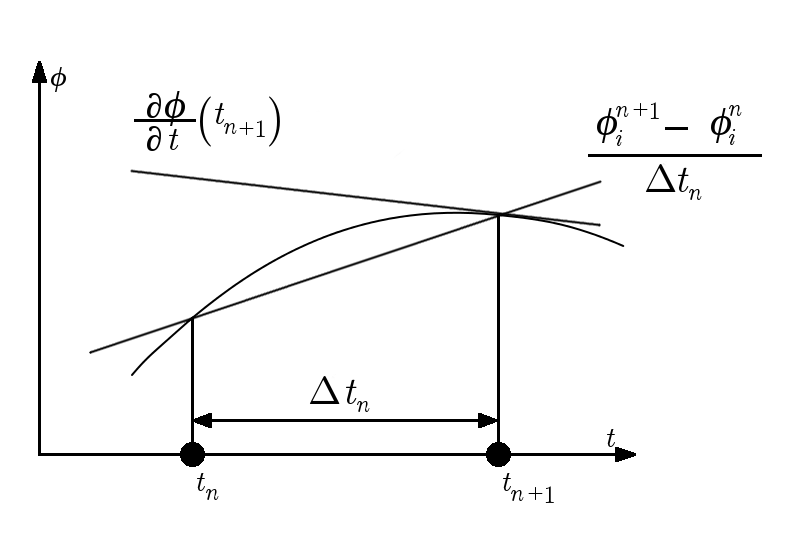
\includegraphics[width=8cm]{Img/5-7}
	\caption{Aproximación Euler hacia atrás}
	\label{img:5-7}
\end{figure}

Por ejemplo, discretizando la ecuación de difusión pura unidimensional (\ref{eq:5-5}) con la discretización espacial de \ref{eq:5-6} y usando el esquema implícito de Euler obtenemos:
\begin{equation}
	\left( 1 + \frac{2 \alpha \Delta t}{\rho \Delta x^2} \right) \phi_P^{n+1} = \frac{\alpha \Delta t}{\rho \Delta x^2} \left( \phi_E^{n+1} + \phi_W^{n+1} \right) + \phi_P^n.
	\label{eq:5-12}
\end{equation}

Considerando todos los volúmenes de control, \ref{eq:5-12} representa un sistema de ecuaciones tridiagonal que debe ser resuelto para cada paso de tiempo.

Para los esquemas implícitos el cambio que generan el contorno en el paso de tiempo actual se expande hacia el centro del dominio (Figura \ref{img:5-8}), lo que evita problemas de estabilidad que fueron indicados para el método explícito de Euler. Por lo tanto el método implícito de Euler es estable independientemente de la discretización espacial ($\Delta x$) y la temporal ($\Delta t$).

A modo de comparación, ambos esquemas (explícito e implícito de Euler) son de primer orden respecto del tiempo ($\Delta t$). El esquema implícito es más costoso computacionalmente y mayor cantidad de memoria, ya que debe resolver un sistema de ecuaciones y almacenar los coeficientes y el término fuente para cada paso de tiempo. Sin embargo no tiene problemas de estabilidad respecto al paso del tiempo, con lo cual para un alto $\Delta t$ compensa el gran costo computacional que tiene.
\begin{figure}[h!]
	\centering
	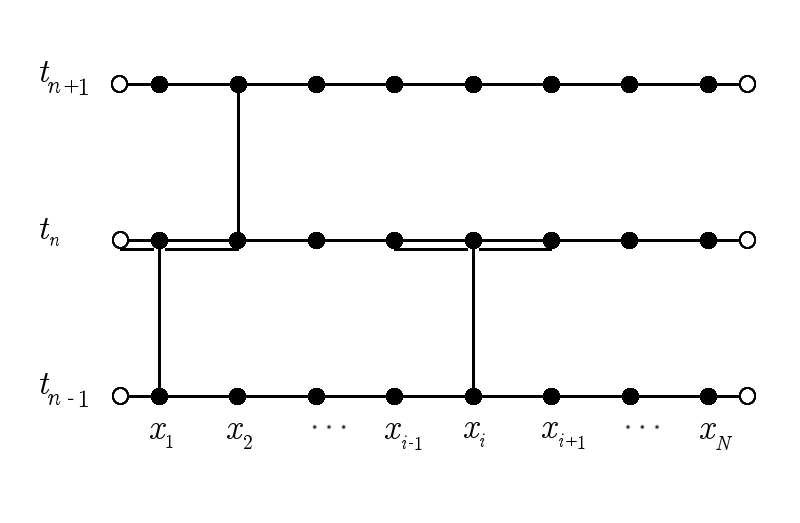
\includegraphics[width=8cm]{Img/5-8}
	\caption{Nodos que utiliza Euler hacia atrás}
	\label{img:5-8}
\end{figure}

El sistema de ecuaciones que resulta de aplicar el método implícito de Euler en la ecuación de transporte para problemas no-estacionarios es:
\begin{equation}
	\left( a_P^{n+1} + \frac{\delta V \rho}{\Delta t_n} \right) \phi_P^{n+1} = \sum_c a_c^{n+1} \phi_c^{n+1} + b_P^{n+1} + \frac{\delta V \rho }{\Delta t_n} \phi_P^n. \nonumber
\end{equation}
Si aplicamos el límite de $\Delta t_n \longrightarrow \infty$ obtenemos la ecuación estacionaria. Entonces, el método puede ser utilizado para ambos casos (estacionario y no-estacionario).

Un esquema implícito frecuentemente utilizado en la práctica es el \textit{método de Crank-Nicolson}, el cual obtiene para cada componente $\phi_i$ en $\phi$ la derivada temporal al instante $t_{n+1/2} = (t_n + t_{n+1})/2$, aproximada utilizando la linea que conecta $\phi_i^{n+1}$ y $\phi_i^n$ (Figura \ref{img:5-9}):
\begin{equation}
	\frac{\partial \phi}{\partial t}(t_{n+1/2}) \approx \frac{\phi^{n+1} -\phi^n}{\Delta t_n} = \frac12 \left[ F(\phi^{n+1} + F(\phi^n) \right]. \nonumber
\end{equation} 
Esta aproximación corresponde a la de diferencias centradas para derivar el tiempo en el instante $t_{n+1/2}$, por lo tanto es de 2do orden de aproximación. 
\begin{figure}[h!]
	\centering
	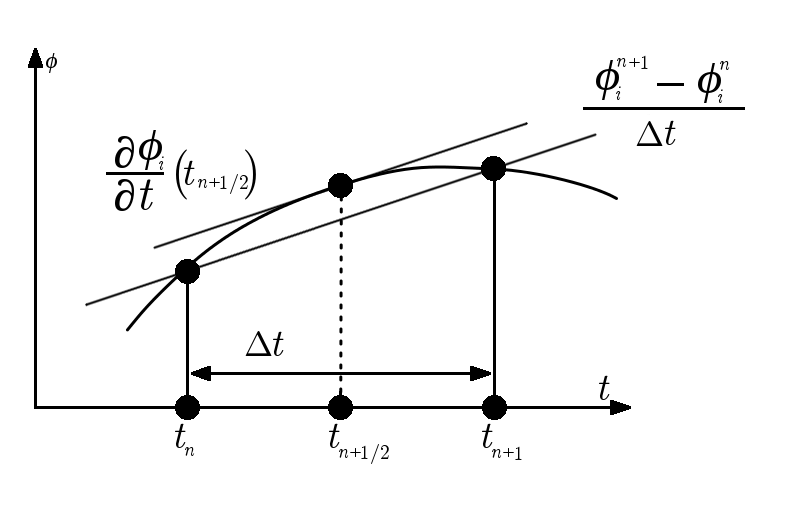
\includegraphics[width=8cm]{Img/5-9}
	\caption{Discretización Crank-Nicolson}
	\label{img:5-9}
\end{figure}

El método de Crank-Nicolson es un poco más costoso que el implícito de Euler, ya que debe calcular $F(\phi^n)$ en el lado derecho de la ecuación y usualmente el sistema de ecuaciones es un poco más complejo de resolver. De todas maneras, el orden de aproximación del Crank-Nicolson es considerablemente mejor.

Para el problema \ref{eq:5-5} con la discretización espacial de \ref{eq:5-6}, el método de Crank-Nicolson resulta:
\begin{equation}
	2 \left( \frac{\alpha \Delta t}{\rho \Delta x^2} \right) \phi_P^{n+1} =  \frac{\alpha \Delta t}{\rho \Delta x^2} \left( \phi_E^{n+1} + \phi_W^{n+1} \right) + \frac{\alpha \Delta t}{\rho \Delta x^2} \left( \phi_E^n + \phi_W^n \right) + 2 \left( 1 - \frac{\alpha \Delta t}{\rho \Delta x^2} \right) \phi_P^n. \nonumber
\end{equation}
Cabe destacar que como todo esquema centrado tiene problemas de estabilidad cuando la solución espacialmente no es suave, lo que genera oscilaciones (no-físicas) en la solución numérica.

Los métodos explícitos e implícitos de Euler y el de Crank-Nicolson pueden ser integrados en una misma ecuación simplemente introduciendo el parametro $\theta$ de la siguiente manera:
\begin{equation}
	\frac{\phi^{n+1} - \phi^n}{\Delta t_n} = \theta F(\phi^{n+1}) + (1-\theta) F(\phi^n). \nonumber
\end{equation}
En la literatura se denomina a esta aproximación como el método de $\theta$. Para $\theta = 0$ y $\theta = 1$ obtenemos el método explícito e implícito de Euler respectivamente. Para $\theta = 1/2$ tenemos el método de Crank-Nicolson. Este método es válido para cualquier discretización temporal para valores $\theta$ en el intervalo $[0,1]$. De todas maneras, solmanete para el valor $\theta = 1/2$ obtenemos una aproximación de 2do orden.

Métodos implícitos multipasos con distintos ordenes son definidos dependiendo de la cantidad de pasos que utilizan, la aproximación en la derivada temporal y la evaluación del término derecho. Un método multi-pasos implícito destacado es el \textit{método-BDF} ( fórmula de diferenciación hacia atrás ). El cual puede ser derivado utilizando una discretización arbitraria de la derivada temporal, con un enfoque hacia atrás involucrando $n$ instantes de tiempo anteriores. En la tabla \ref{table52} se muestran las aproximaciones con sus respectivos ordenes.

$~$

\begin{table}[h!]
\centering
\begin{tabular}{| l c |}
\hline
Fórmula & Orden \\
\hline
 & \\
$\frac{\phi^{n+1} - \phi^n}{\Delta t} = f(\phi^{n+1}) $ & 1 \\
 & \\
$\frac{3 \phi^{n+1} - 4 \phi^n + \phi^{n-1}}{2 \Delta t} = f(\phi^{n+1}) $ & 2 \\
 & \\
$\frac{11 \phi^{n+1} - 18 \phi^n + 9 \phi^{n-1} + 2 \phi^{n-2}}{6 \Delta t} = f(\phi^{n+1}) $ & 3 \\
 & \\
$\frac{25 \phi^{n+1} - 48 \phi^n + 36 \phi^{n-1} - 16 \phi^{n-2} + 3 \phi^{n-3}}{2 \Delta t} = f(\phi^{n+1}) $ & 4 \\
 & \\
\hline
\end{tabular}
\caption{Orden de aproximación de los diferentes métodos implícitos multipasos.}
\label{table52}
\end{table}

$~$

\pagebreak

Otro esquema implícito multi-pasos es el \textit{método de Adams-Moulton}, su correspondiente formulación está en la tabla \ref{tabla53}. Los primero ordenes (1er y 2do) del método de Adams-Moulton corresponden al método implícito de euler y al de Crank-Nicolson. 

El método de Adams-Moulton puede ser utilizado en conjunto con el de Adams-Bashforth como un método de \textit{predictor-corrector}. Donde el esquema explícito es el predictor y el implícito es el corrector. Por ejemplo, el correspondiente esquema predictor-corrector de 4to orden esta dado por:
\begin{eqnarray}
	\phi^* = \phi^n + \frac{\Delta t}{24} \left[ 55 F(\phi^n) -29 F(\phi^{n-1}) + 37 F(\phi^{n-2}) - 9F(\phi^{n-3}) \right], \nonumber \\
	\phi^{n+1} = \phi^n + \frac{\Delta t}{24} \left[ 9 F(\phi^*) + 19 F(\phi^n) - 5 F(\phi^{n-1}) + F(\phi^{n-2}) \right]. \nonumber
\end{eqnarray}

$~$

\begin{table}[h]
\centering
\begin{tabular}{| l c |}
\hline
Fórmula & Orden \\
& \\
$\frac{\phi{n+1} - \phi^n}{\Delta t} = f(\phi^{n+1})$ & 1 \\
& \\
$\frac{\phi{n+1} - \phi^n}{\Delta t} = \frac12 \left[ f(\phi^{n+1}) + f(\phi^{n})\right]$ & 2 \\
& \\
$\frac{\phi{n+1} - \phi^n}{\Delta t} = \frac{1}{12} \left[ 5 f(\phi^{n+1}) + 8 f(\phi^{n}) - f(\phi^{n-1}) \right] $ & 3 \\
& \\
$\frac{\phi{n+1} - \phi^n}{\Delta t} = \frac{1}{24} \left[ 9 f(\phi^{n+1}) +19 f(\phi^n) -5 f(\phi^{n-1}) + f(\phi^{n-2}) \right]$ & 4 \\
& \\
\hline
\end{tabular}
\caption{Orden de aproximación de los métodos implícitos Adams-Moulton}
\label{tabla53}
\end{table}

\chapter{Solución algebraica para sistema de ecuaciones}

La discretización para problemas estacionario o no-estacionarios con una integración implícita en el tiempo, en conjunto con el método de volúmenes finitos se obtiene un sistema de ecuaciones algebraico. El proceso de solución para este tipo de sistemas es de gran importancia, ya que frecuentemente el 50\% o más del costo computacional total es requerido por la solución numérica del sistema. Por lo tanto, en este capítulo trataremos con detalle métodos que resuelven estos sistemas considerándolos lineales.

\section{Sistemas lineales}

El sistema de ecuaciones lineales puede ser resuelta a partir de su forma general:
\begin{equation}
	a^i_P \phi^i_P - \sum_c a_c^i \phi_c^i = b_P^i ~~ para ~ i=1,..n,
	\label{eq:6-1}
\end{equation}
donde la sumatoria con indice $c$ hace referencia a los nodos en el vecindario de $P$. En notación matricial definimos al sistema \ref{eq:6-1} como
\begin{equation}
	\mathbf{A \phi = b}.
	\label{eq:6-2}
\end{equation}
La estructura de la matriz $\mathbf{A}$ en el sistema, es determinada principalmente por el esquema de discretización utilizado, la dimensión $n$ está ligada a la cantidad de variables desconocida en los nodos.

El sistema matricial se genera a partir del método de discretización e imponiendo las condiciones de contorno, de esta manera obtenemos un sistema no-singular que tiene una única solución. In principio hay dos posibilidades numéricas para resolver el sistema:
\begin{itemize}
	\item[$\bullet$] Métodos directos,
	\item[$\bullet$] Métodos iterativos.
\end{itemize}
La característica de los métodos directos es que obtienen la solución \textit{exacta} del sistema sin utilizar algún tipo de algoritmo, en cambio, los métodos iterativos \textit{aproximan} la solución repitiendo iterativamente una secuencia de pasos.

\section{Métodos Directos}

Para evaluar los métodos directos tomemos como punto de partida la \textit{eliminación Gausiana}. A pesar de su alto costo computacional, algunas veces es utilizado en mecánica estructural bajo la estructura del Método de Elementos Finitos. Una variación importante es la descomposición $\mathbf{LU}$ de la matriz $\mathbf{A}$, la cual consta en generar dos matrices triangulares inferior ($\mathbf{L}$) y superior ($\mathbf{U}$) de manera que:
\begin{equation}
	A = 
	\underbrace{	
	\begin{bmatrix}
		1 		& 0 & . & . & . & 0 \\
		l_{21} 	& . & . & ~ & ~ & . \\
		. 	& . & . & . & ~ & . \\
		. 	& ~ & . & . & . & . \\
		. 	& ~ & ~ & . & . & 0 \\
		l_{K,1} 	& . & . & ~ & l_{K,K-1} & 1 
	\end{bmatrix}}_{\mathbf{L}}
	\underbrace{
	\begin{bmatrix}
		u_{1,1} 	& u_{1,2} & . & . & . & u_{1,K} \\
		0 & . & . & ~ & ~ & . \\
		. 	& . & . & . & ~ & . \\
		. 	& ~ & . & . & . & . \\
		. 	& ~ & ~ & . & . & u_{K-1,K} \\
		0 	& . & . & ~ & 0 & u_{K,K} 
	\end{bmatrix}}_{\mathbf{U}}. \nonumber
\end{equation}

donde los coeficientes $l_{i,j}$ y $u_{i,j}$ tienen que ser calculados en el proceso de eliminación. Luego de realizar la eliminación, la solución del sistema se basa en realizar un proceso de sustitución hacia delante y hacia atrás. Primero el sistema:
\begin{equation}
	\mathbf{Lh = b} \nonumber
\end{equation}
es resuelto haciendo la sustitución hacia delanta para $\mathbf{h}$ y luego la solución para $\phi$ es determinada por
\begin{equation}
	\mathbf{U \phi = h} \nonumber
\end{equation}
la sustitución hacia atrás.

Si $\mathbf{A}$ es una matriz banda, como lo es usualmente en los casos de discretización que hemos visto (ver 4.6 ejemplo de volúmenes finitos), las matrices $\mathbf{L}$ y $\mathbf{U}$ también son bandas (con el mismo ancho que $\mathbf{A}$). Pero dentro de dicha banda, la matriz $\mathbf{A}$ no está completamente llena, cosa que no sucede con sus matrices $\mathbf{L}$ y $\mathbf{U}$ que generalmente están llenas dentro de la banda. Esto es una desventaja crucial para los métodos directos cuando se están aplicando sobre problemas de dos y tres dimensiones. Para matrices tridiagonales la eliminación de Gaus es conocida en la literatura como \textit{TDMA} (algoritmo para matrices tridiagonales) o \textit{algoritmo de Thomas}.

Para matrices simétricas y definidas positivas existe una variante de la eliminación llamada como el \textit{método de Cholesky}. El cual mejora el orden de las operaciones y es menos sensible al error de redondeo.

\section{Métodos iterativos}

Los métodos iterativos comienzan con una estimación a la solución $\phi^0$, la cual es sucesivamente mejorada por la aplicación iterativa del proceso $P$:
\begin{equation}
	\phi^{k+1} \longleftarrow P(\phi^k), ~ k=0,1,... \nonumber
\end{equation}
El \textit{método de Jacobi} y el \textit{método de Gaus-Seidel} son los métodos iterativos más simples. El primero, propone obtener una mejor solución insertando los valores $\phi^k$ (``viejos" ) en el término de la sumatoria de la ecuación algebraica (\ref{eq:6-1}), obteniendo un nuevo valor para el nodo $P$ a partir de los valores de sus vecinos, matemáticamente:
\begin{equation}
	\phi_P^{i,k+1} = \frac{1}{a_P^i} \left( \sum_c a_c^i \phi_c^{i,k} + b_P^i \right). \nonumber
\end{equation}
En la figura \ref{img:6-1} se ilustra el proceso para problemas en dos dimensiones utilizando la discretización de Volúmenes Finitos. Las propiedades del método de Jacobi son completamente independientes de la cantidad de variables.

La convergencia del método de Jacobi puede ser mejorada si cuando se está calculando el nuevo valor para P, uno de sus vecinos involucrados en la discretización ya tiene asignado el nuevo valor. Esto lleva al método de \textit{Gaus-Seidel}:
\begin{equation}
	\phi_P^{i,k+1} = \frac{1}{a_p^i} \left( \sum_{c_1} a_{c_1}^i \phi_{c_1}^{i,k} + \sum_{c_2} a_{c_2}^i  \phi_{c_2}^{i,k+1} + b_P^i \right), \nonumber  
\end{equation}
donde el índice $c_1$ indica los nodos que no fueron calculados y el índice $c_2$ para los que tiene los nuevos valores. Proceso ilustrado en la figura \ref{img:6-1}:
\begin{figure}[h!]
	\centering
	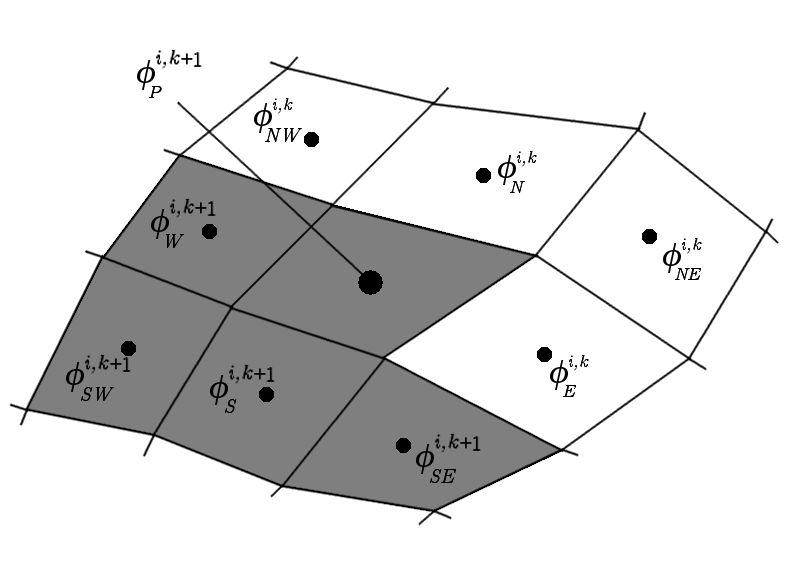
\includegraphics[width=8cm]{Img/6-1}
	\caption{Proceso de iteración \textit{k+1} en P, Gaus-Seidel}
	\label{img:6-1}
\end{figure}

Para que los métodos de Jacobi y de Gaus-Seidel converjan a una solución, la matriz $A$ del sistema tiene que ser \textit{diagonal dominante}, es decir, para todo $i=1,..,n$ se debe cumplir la siguiente inecuación:
\begin{equation}
	\mid a_P^i \mid \geq \sum_c \mid a_c^i \mid. \nonumber
\end{equation}
Por ejemplo para resolver la ecuación de transporte escalar no-estacionaria (\ref{eq:5-5}) unidimensional con un esquema implícito como el de Euler (\ref{eq:5-12}), observamos que los coeficientes de los nodos interiores tienen los siguientes valores:
\begin{equation}
a_P = 2 \frac{\alpha \Delta t}{ \rho \Delta x^2} + 1 ~~ ;~~ a_W = a_E = \frac{\alpha \Delta t}{ \rho \Delta x^2}, \nonumber
\end{equation}
es de notar que al acoplar las ecuaciones, la matriz $A$ es diagonal dominante. 

La taza de convergencia del método de Gaus-Seidel puede ser mejorada bajo una relajación, resultando el \textit{método SOR (sobre-relajación sucesiva)}. Los valores $\phi_*^{k+1}$ son obtenidos utilizando el método de Gaus-Seidel, luego son combinados linealmente con los valores anteriores $\phi^k$ para obtener el nuevo valor de la iteración:
\begin{equation}
	\phi^{k+1} = \phi^k + \omega (\phi_*^{k+1} - \phi^k), \nonumber
\end{equation}
donde el parámetro de relajación $\omega$ debe estar en el intervalo $[1,2)$. Para $\omega = 1$ obtenemos el método de Gaus-Seidel. El método SOR se representa de la siguiente manera:
\begin{equation}
	\phi_P^{i,k+1} = (1-\omega)\phi_P^{i,k} + \frac{\omega}{a_P^i} \left( \sum_{c_1} a^i_{c_1} \phi_{c_1}^{i,k} + \sum_{c_2} a_{c_2}^i \phi_{c_2}^{i,k+1} + b_P^i \right).
\end{equation}
De manera general no es posible especificar un valor óptimo $\omega_{opt}$ para el parámetro de relajación $\omega$ de manera explícita. Este valor puede obtenerse teóricamente para modelos lineales sencillos, en estos casos el método SOR reduce considerablemente el costo computacional respecto al método de Gaus-Seidel, simplemente introduciendo el coeficiente de relajación.

\subsection{Gradiente Conjugado}

Un importante método iterativo para resolver sistemas lineales es el \textit{método del gradiente conjugado(MGC)}. La idea básica es resolver un problema de minimización el cual es equivalente al sistema de ecuaciones original. Existen muchas variantes del método, las cuales principalmente se diferencian en como se formula el problema de minimización y la búsqueda del mínimo error.

El MGC fue desarrollado para resolver sistemas lineales para los cuales su matriz $A$ es simétrica definida positiva, teniendo en cuenta la siguiente equivalencia:
\begin{equation}
	Resolver ~~ \mathbf{A \phi = b} ~~ \Leftrightarrow ~~ Minimizar ~ F(\phi) = \frac12 \mathbf{\phi \cdot A \phi - b \cdot \phi}. \nonumber
\end{equation}
La equivalencia en ambas formulaciones se ve fácilmente, mientras que el gradiente de $F$ es $\mathbf{A \phi - b}$, y anular el gradiente es la condición necesaria para minimizar $F$.

Para una solución iterativa en la minimización del problema, comienza con un valor inicial $\phi^0$ arbitrario. La función $F$ es minimizada sucesivamente por cada iteración ($k=0,1..$) en direcciones de $y^k$:
\begin{equation}
	Minimize ~~ F(\phi^k + \alpha y^k) ~ \forall ~ real ~ \alpha. \nonumber
\end{equation}
El valor $\alpha^k$, para los que la función alcanza su mínimo resulta:
\begin{equation}
	\frac{d}{d \alpha} F(\phi^k + \alpha \mathbf{y^k}) = 0 ~~ \Rightarrow ~~ \alpha^k = \frac{\mathbf{y \cdot r^k}}{\mathbf{y^k \cdot A y^k}} ~~ con ~ \mathbf{r^k = b - A \phi^k} \nonumber
\end{equation}
y define el nuevo valor de la iteración es $\phi^{k+1} = \phi^k + \alpha^k y^k$. Las direcciones $y^k$, in la búsqueda del mínimo, se caracteriza por el hecho de que se conjuga con respecto a $\mathbf{A}$ para todas las direcciones anteriores,
\begin{equation}
	\mathbf{y^k \cdot A y^i} = 0 ~~ \forall ~ i=0,..,k-1. \nonumber
\end{equation}
Para una implementación eficiente del MGC, las direcciones de búsqueda $\mathbf{y^{k+1}}$ se deben definir de acuerdo a la siguiente fórmula:
\begin{equation}
	\mathbf{y^{k+1}} = \mathbf{r^{k+1}} + \frac{\mathbf{r^{k+1} \cdot r^{k+1}}}{\mathbf{r^k \cdot r^k}} \mathbf{y^{k}}. \nonumber
\end{equation}

De esta manera, definimos el algoritmo del MGC:

\begin{itemize}
	\item[$\bullet$] Inicialización:
			\begin{eqnarray}
				r^0 = b - A \phi^0 , \nonumber \\
				y^0 = r^0 , \nonumber \\
				\beta^0 = r^0 \cdot r^0 . \nonumber
			\end{eqnarray}
	
	\item[$\bullet$] Para k=0,1, ... hasta la convergencia:
			\begin{eqnarray}
				\alpha^k = \beta^k / (y^k . A y^k), \nonumber \\
				\phi^{k+1} = \phi^k + \alpha^k y^k, \nonumber \\
				r^{k+1} = r^k - \alpha^k A y^k, \nonumber \\
				\beta^{k+1} = r^{k+1} \cdot r^{k+1}, \nonumber \\
				y^{k+1} = r^{k+1} + \beta^{k+1} y^k / \beta^k. \nonumber
			\end{eqnarray}
\end{itemize}

El MGC esta libre de parámetros y teóricamente obtiene la solución exacta después de $N$ iteraciones, donde $N$ es la cantidad de variables en el sistema. 


\chapter{Métodos implementados}

En el capítulo dos planteamos las bases para desarrollar el modelo matemático de Navier-Stokes para fluidos newtonianos incompresibles, para el cual resta definir la manera de acoplar los campos de presión y velocidad, dicho acople, se realiza de diversos modos dependiendo el método utilizado, en nuestro caso, implementamos los métodos SIMPLE (Método Semi-Implícito para Acoplar la Presión) y el Fractional-Step (Pasos Fraccionados), los cuales son métodos de \textit{predicción-corrección} y haremos referencia a ellos como los ``métodos implementados".

La primera etapa consta de discretizar la geometría, en el capítulo 3 desarrollamos las diferentes posibilidades de discretización utilizando elementos cuadrados o triángulos; un caso particular es utilizar \textit{mallas desplazadas} para evitar un fenómeno no-físico denominado \textit{checkerboard} que se produce en mallas con elementos cuadrados estructurados. El siguiente paso, es discretizar las ecuaciones del modelo matemático, para ello en el capítulo 4 se introdujo el método integral de Volúmenes Finitos, el cual discretiza los términos de convección, difusión y el de presión evaluando el flujo en las fronteras. Dado que este tipo de problema no es estacionario, en el capítulo 5 desarrollamos los modos de discretización temporal, para los cuales se implementó el Adams-Bashforth (explícito) y el Backward-Euler (implícito). Este último genera como resultado, un sistema de ecuaciones lineales que será resuelto con el método de Gaus-Seidel desarrollado en el capítulo 6, además los métodos implementados necesitan resolver un sistema de ecuaciones en la etapa de corrección, dicho sistema genera una matriz simétrica definida positiva que se resuelve en n iteraciones con el método del Gradiente conjugado.

\section{Mallas desplazadas}

Comenzamos discretizando el espacio físico como lo hace normalmente el método de volúmenes finitos (en elementos de control), luego ubicamos las variables escalares (presión, temperatura, etc) y vectoriales (velocidad) en el centroide de cada volumen de control como se hace normalmente. 
\begin{figure}[h!]
  \centering
  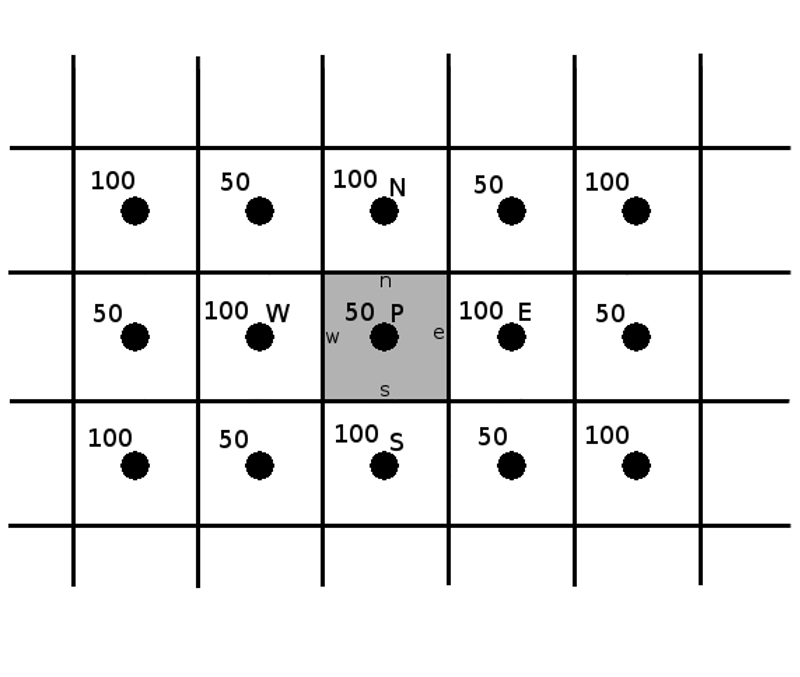
\includegraphics[width=8cm]{Img/7-1}
  \caption{Problema ``checkerboard"}
  \label{fig:7-1}
\end{figure}
Pero esto puede generar un campo de presión no uniforme (``checker-board") que actúa en la ecuación de momento discretizada como un campo uniforme. Esto puede ser demostrado con un ejemplo sencillo en dos dimensiones, utilizando una grilla con elementos cuadrados estructurados, supongamos que obtenemos esta no uniformidad en el campo de presión con los valores que muestra la figura \ref{fig:7-1}. 

Si las presiones en w y e son obtenidas mediante una interpolación lineal, el gradiente de presión ($\partial p / \partial x$) en la ecuación de momento en la dirección $x$ está dado:
\begin{equation}
  \frac{\partial p}{\partial x} = \frac{p_e - p_w}{\delta x} = \frac{ (p_E + p_P)/2 - (p_W + p_P)/2}{\delta x} = \frac{p_E - p_W}{2 \delta x},
  \label{eq:presionCheckx}
\end{equation}
de manera similar obtenemos el gradiente de presión para la ecuación de momento en $y$:
\begin{equation}
  \frac{\partial p}{\partial y} = \frac{p_N - p_S}{2 \delta y}.
  \label{eq:presionChecky}
\end{equation}

En las ecuaciones \ref{eq:presionCheckx} y \ref{eq:presionChecky}, el nodo central P no realiza ningún aporte para el cálculo del gradiente de presión en su volumen de control. Si reemplazamos apropiadamente los valores del campo ``checker-board" \ de presión que muestra
\begin{figure}[h!]
  \centering
  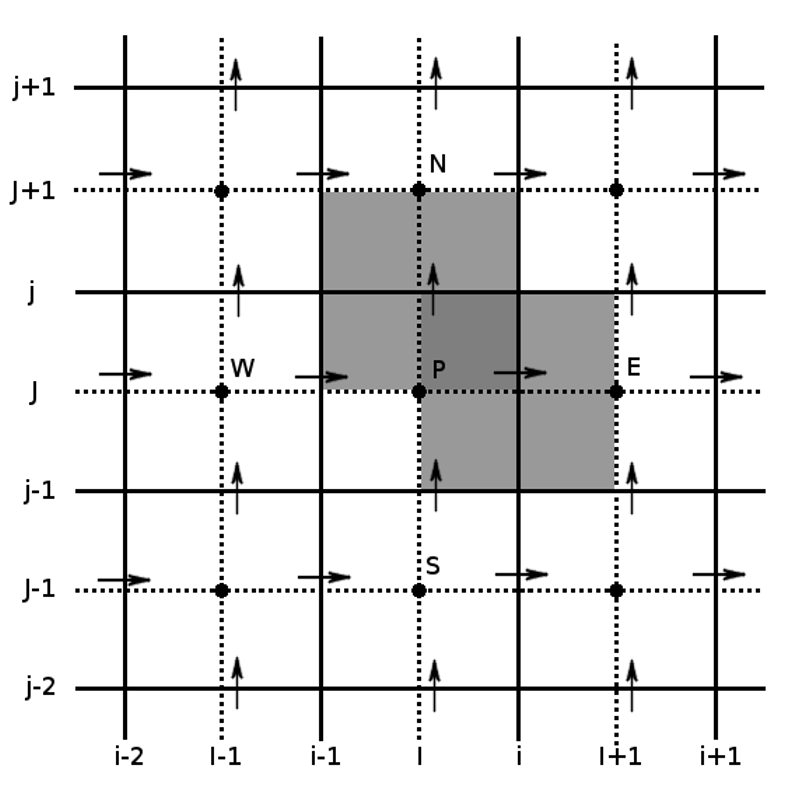
\includegraphics[width=8cm]{Img/7-2}
  \caption{Malla desplazada (Staggered-grid)}
  \label{fig:7-2}
\end{figure}
la figura \ref{fig:7-1} en las ecuaciones de momento \ref{eq:presionCheckx} y \ref{eq:presionChecky}, obtenemos que todos los gradientes de presión son nulos en ambas direcciones. Este campo con forma de ``checker-board" \ genera el mismo aporte en el término fuente que un campo de presión uniforme, pero claramente no es un comportamiento físico real.

En consecuencia, si el campo de velocidad está asignado en la misma posición que las variables escalares, el campo de presión no se encuentra correctamente representado en la ecuación de momento. Una solución para este tipo de problemas es utilizar \textit{staggered grid} (mallas desplazadas) para las componentes de velocidad (Harlow and welch, 1995). Este concepto consta de evaluar las variables escalares en los nodos como se hace normalmente, pero el campo de velocidad se calcula en la malla desplazada centrada en las caras de los volúmenes de control como muestra la figura \ref{fig:7-2}, donde las variables escalares se encuentran en los nodos indicados por \textbullet $~$ y las variables pertenecientes al campo de velocidad se encuentran las caras de los elementos entre las variables escalares, se representan en la imagen con $\longrightarrow$ y $\uparrow$, para la componente en dirección $u$ (Figura \ref{fig:7-3}) y $v$ (Figura \ref{fig:7-4}) respectivamente. Las letras $E$, $W$, $N$ y $S$ hacen referencia a los vecinos este, oeste, norte y sur de P; los campos de velocidad se encuentran en w y e para $u$, en s y n para $v$.  De esta manera los volúmenes de control para las variables escalares son diferentes que los del campo de velocidad.
\begin{figure}[h!]
  \centering
  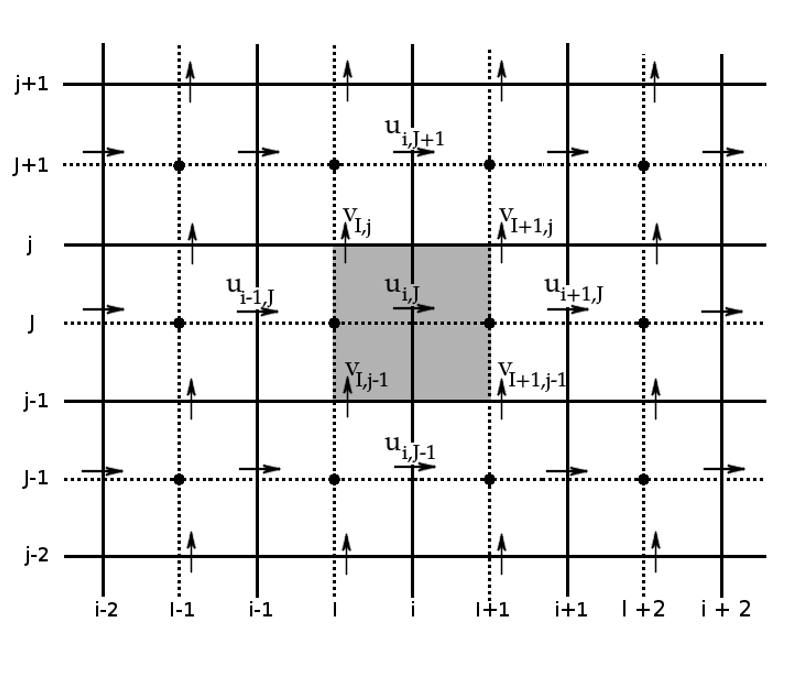
\includegraphics[width=8cm]{Img/7-3}
  \caption{Elemento de velocidad u}
  \label{fig:7-3}
\end{figure}

\begin{figure}[h!]
  \centering
  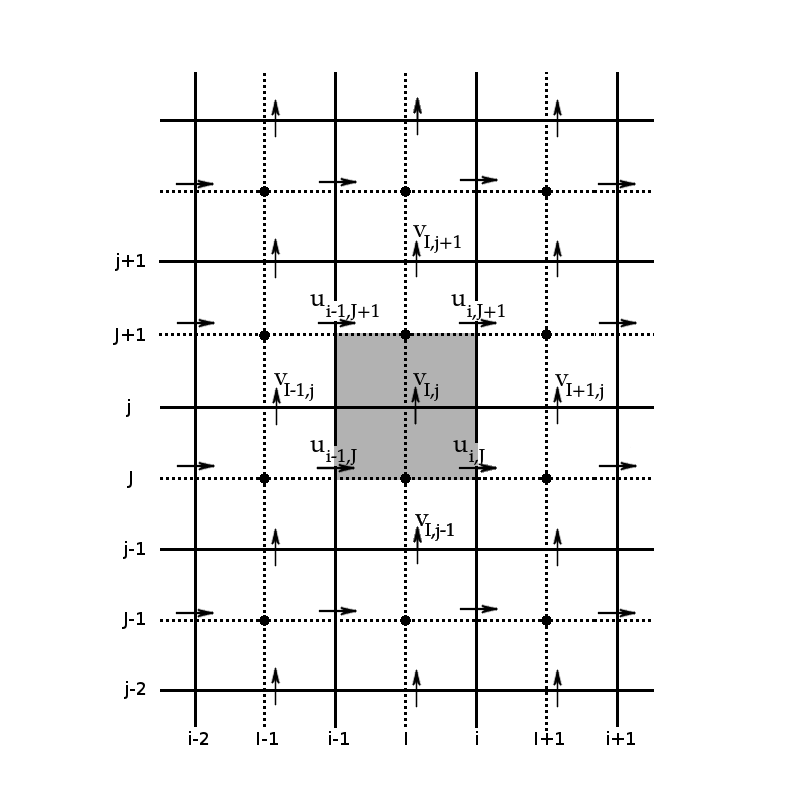
\includegraphics[width=8cm]{Img/7-4}
  \caption{Elemento de velocidad v}
  \label{fig:7-4}
\end{figure}

Utilizando las mallas desplazadas los nodos de presión están ubicados en las caras de los volúmenes del campo de velocidad, para la componente $u$ el gradiente de presión está dado:
\begin{equation}
  \frac{\partial p}{\partial x} = \frac{p_P - p_W}{ \delta x},
  \label{eq:presionCheckyu}
\end{equation}
de la misma manera para la componente $v$:
\begin{equation}
  \frac{\partial p}{\partial y} = \frac{p_P - p_S}{ \delta y}.
  \label{eq:presionCheckyv}
\end{equation}

Si nuevamente consideramos el caso del ``checker-board" \ y sustituyendo los valores (figura \ref{fig:7-1}) en las ecuaciones \ref{eq:presionCheckyu} y \ref{eq:presionCheckyv} los gradientes dejan de ser nulos. Por lo tanto, el uso de las mallas desplazadas evita las oscilaciones irreales del tipo ``checker-board" \ en el campo de presión, además que se evita realizar interpolaciones para obtener las velocidades en las caras.

\section{Discretización por Volúmenes Finitos}

Luego de tener el dominio del problema subdividido en elementos, planteamos la conservación local de la ecuación \ref{eq:2-7}. Como el fluido es incompresible el término convectivo para la componente $u$ puede ser escrito como $\nabla \cdot (\rho \mathbf{v} u )$, de esta manera integramos sobre el volumen:
\begin{equation}
	\int_V  \rho \frac{\partial u}{\partial t} dV + \int_V  \nabla  \cdot \left( \rho \mathbf{v} u \right) dV = \int_V - \nabla p dV + \int_V  \mu \Delta u dV. \nonumber
\end{equation}
Aplicando el teorema de la divergencia:
\begin{equation}
	\int_V  \rho \frac{\partial u}{\partial t} dV + \oint_S  \left( \rho \mathbf{v} u \right) \cdot \mathbf{n} dS = \oint_S - p \mathbf{n}_x dS + \oint_S \mu \nabla u \cdot \mathbf{n} dS. \nonumber
\end{equation}
Todas las integrales excepto la temporal dependen del contorno o superficie del elemento. La integral volumétrica en el término temporal se discretiza con la hipótesis de que el valor de velocidad en todo el elemento es constante por lo tanto no depende del espacio local. Pero si depende del tiempo y se discretiza utilizando una aproximación de primer orden:
\begin{equation}
	\int_V  \rho \frac{\partial u}{\partial t} dV = \frac{u^{n+1} - u^n}{\delta t} \delta V. \nonumber
\end{equation}
Por otro lado, las integrales de superficie son discretizadas con la regla del punto medio, de esta manera los términos convectivos, difusivos y de presión quedan:
\begin{equation}
	\sum_n \rho \left( \mathbf{v} u \right)_n \cdot \mathbf{n}_n \delta S_n ~ ; ~ \sum_n \mu ( \nabla u \cdot \mathbf{n} )_n  \delta S_n; ~ - \sum_n ( p \mathbf{n}_x )_n \delta S_n ~ ;  \nonumber
\end{equation}
donde el subíndice $n$ indica el punto medio de cada frontera, el cual debe interpolarse utilizando los valores de los elementos que comparten dicha frontera. El término convectivo se trata de manera cautelosa ya que puede provocar inestabilidad, en los métodos implementados se utilizó el esquema UPWIND de primer orden, el cual evalúa la dirección del campo de velocidad en la frontera, el cual se obtiene interpolando:
\begin{equation}
	 \mathbf{v}_n = \alpha_N \mathbf{v}_N + \alpha_P \mathbf{v}_P, \nonumber
\end{equation}
donde $\alpha_N = d_{Nn} / d_{NP}$ es el cociente entre la distancia del centroide vecino $N$ con el centro de la arista $n$ y la distancia entre los centroide de los elementos $N$ y $P$. El esquema UPWIND define la velocidad en la frontera como:
\begin{equation}
	\rho (\mathbf{v} \cdot \mathbf{n})_n u_\Gamma \delta S_n   
	\left\lbrace
	\begin{array}{l}
		u_\Gamma = u_P \text{ if }  (\mathbf{v} \cdot \mathbf{n})_n > 0\\
		u_\Gamma = u_N \text{ if }  (\mathbf{v} \cdot \mathbf{n})_n < 0\\
	\end{array}
	\right. \nonumber
\end{equation}
El término difusivo se calcula aproximando la primera derivada en la frontera utilizando un esquema centrado de segundo orden:
\begin{equation}
	\mu ( \nabla u \cdot \mathbf{n} )_n  \delta S_n = \mu \left( \frac{u_N - u_P}{(\mathbf{x}_N - \mathbf{x}_P) \cdot \mathbf{n}_n } \right) \delta S_n. \nonumber
\end{equation}
Por último el término de presión, el cual para mallas estructuradas con mallas staraged la presión en la frontera es conocida, por lo tanto no se necesita ningún tipo de interpolación, pero para mallas no estructuradas se debe interpolar de la siguiente manera:
\begin{equation}
	( p \mathbf{n}_x )_n \delta S_n = (\alpha_N p_N + \alpha_P p_P) \mathbf{n}_x \delta S_n, \nonumber
\end{equation}

Una vez discretizado todos los términos, presentamos la ecuación completa con un esquema temporal implísito:
\begin{eqnarray}
	\frac{u^{n+1} - u^n}{\delta t} \delta V + \sum_n \rho (\mathbf{v} \cdot \mathbf{n})_n u_\Gamma^{n+1} \delta S_n - \sum_n \mu \left( \frac{u_N^{n+1} - u_P^{n+1}}{(\mathbf{x}_N - \sum_n \mathbf{x}_P) \cdot \mathbf{n}_n } \right) \delta S_n \nonumber \\
	= - \sum_n (\alpha_N p_N^{n+1} + \alpha_P p_P^{n+1}) \mathbf{n}_x \delta S_n.
	\label{eq:7-5}
\end{eqnarray}

La ecuación \ref{eq:7-5} representa la discretización por el MVF de la ecuación de Navier-Stokes para fluidos newtonianos incompresibles (\ref{eq:2-7}). A continuación explicaremos como los métodos implementados desacoplan los campos de presión y velocidad.


\section{SIMPLE}

El método iterativo SIMPLE fue propuesto por Patankar y Spalding (1972), y consiste en utilizar un campo de presión y velocidad inicial ``adivinado" $~$para resolver la ecuación de momento y la de corrección del campo de presión. Esta última deducida de la ecuación de continuidad, la cual es utilizada para corregir los campos de presión y velocidad. Para dar inicio a las iteraciones se utiliza un capo de presión y velocidad inicial ``adivinado", por ejemplo, si el fluido parte de un estado en completo reposo, ambos campos son nulos. Se resuelve la ecuación de momento, se obtiene el campo de corrección y se termina la iteración corrigiendo los campos de presión y velocidad. El método itera constantemente hasta que el fluido llegue al estado estacionario, numéricamente hasta que los campos de presión y velocidad converjan, es decir para la iteración en $n+1$ tenemos que:
\begin{equation}
	u^{n+1} \approx u^n, ~~ v^{n+1} \approx v^n ~~y~~ p^{n+1} \approx p^n. \nonumber
\end{equation}

\subsection{Algoritmo SIMPLE}

El método SIMPLE consta de ``adivinar" $~$y corregir el campo de presión y velocidad. El proceso iterativo comienza adivinando el campo de presión $p^*$ para resolver las ecuaciones de momento y obtener un campo los campos de velocidad $u^*$ y $v^*$, para luego corregirlos. De manera general, escribimos las ecuaciones de momento:
\begin{equation}
  a_{P}u_{P}^* = \sum a_{n}u_{n}^* + \sum p^*_n \mathbf{n}_x S_n,
  \label{eq:momentoSIMPLEu}
\end{equation}
\begin{equation}
  a_{P}v_{P}^* = \sum a_{n}v_{n}^* + \sum p^*_n \mathbf{n}_y S_n,
  \label{eq:momentoSIMPLEv}
\end{equation}
donde los coeficientes $a_i$ dependen los esquemas de difusión y convección empleados, $p_n$ es la presión en la frontera $n$, $S_n$ es la superficie de intercambio y $\mathbf{n}$ es la normal de la frontera.

Definimos:
\begin{equation}
  p = p^* + p',
  \label{eq:correccionp}
\end{equation}
donde $p'$ es la corrección al campo de presión y $p$ es el campo de presión correcto. De manera similar:
\begin{equation}
  u = u^* + u',
  \label{eq:correccionu}
\end{equation}
\begin{equation}
  v = v^* + v'.
  \label{eq:correccionv}
\end{equation}

Para un campo de presión ($p$) correcto se obtiene el valor exacto del campo de velocidades ($u,v$), si restamos las ecuaciones que utilizan los correctos campos de presión y velocidad con los campos ``adivinados" del SIMPLE obtenemos:
\begin{eqnarray}
  \lefteqn{a_{P}(u_{P} - u_{P}^*) = \sum a_{n}(u_{n} - u_{n}^*)} \nonumber \\
  && + \sum (p_n - p^*_n) \mathbf{n}_x S_n, \nonumber \\
  \lefteqn{a_{P}(v_{P} - v_{P}^*) = \sum a_{n}(v_{n} - v_{n}^*) } \nonumber \\
  && + \sum (p_n - p^*_n) \mathbf{n}_y S_n. \nonumber
\end{eqnarray}

Utilizando las ecuaciones de corrección (\ref{eq:correccionp}, \ref{eq:correccionu} y \ref{eq:correccionv}), las ecuaciones anteriores pueden ser reescritas como:
\begin{eqnarray}
  a_{P}u_{P}^\prime = \sum a_{n} u_{n}^\prime + \sum p_n^\prime \mathbf{n}_x S_n, \nonumber \\
  a_{P}v_{P}^\prime = \sum a_{n} v_{n}^\prime + \sum p_n^\prime \mathbf{n}_y S_n. \nonumber
\end{eqnarray}

A modo de simplificación se eliminan los términos $\sum a_{n}u_{n}^\prime$ y $\sum a_{n}v_{n}^\prime$ de las ecuaciones anteriores. La omisión de estos términos es la principal aproximación del algoritmo SIMPLE. Por lo tanto, obtenemos:
\begin{eqnarray}
  u_{P}^\prime = \frac{\sum p_n^\prime \mathbf{n}_x S_n}{a_P}, \nonumber \\
  v_{P}^\prime = \frac{\sum p_n^\prime \mathbf{n}_y S_n}{a_P}.
  \label{eq:SimpleCorreccion1}
\end{eqnarray}
Sustituyendo en las ecuaciones \ref{eq:correccionu} y \ref{eq:correccionv} obtenemos las ecuaciones para la corrección del campo de velocidades, las cuales se expresan:

\begin{eqnarray}
  u_{P} = u_{P}^* + \frac{\sum p_n^\prime \mathbf{n}_x S_n}{a_P}, \nonumber\\
  v_{P} = v_{P}^* + \frac{\sum p_n^\prime \mathbf{n}_y S_n}{a_P}.
  \label{eq:SimpleCorreccion2}
\end{eqnarray}

Hasta ahora solo hemos trabajado sobre la ecuación de momento, pero como fue mencionado anteriormente, el campo de velocidades está sujeto a la restricción que impone la ecuación de continuidad o de incompresibilidad.
\begin{equation}
  \nabla \cdot \textbf{u} = 0,
  \label{eq:continuidadSimple}
\end{equation}
Integrando en el volumen y aplicando el teorema de la divergencia obtenemos:
\begin{equation}
	\int \nabla \cdot \textbf{u} dV = \oint \mathbf{u} \cdot \mathbf{n} dS. \nonumber
\end{equation}
Aproximando la integral con el método del punto medio y evaluando las $n$ caras obtenemos:
\begin{equation}
	\int \nabla \cdot \textbf{u} dV = \sum_n \mathbf{u} \cdot \mathbf{n}_n dS_n
\end{equation}
Para elementos cuadrados como muestra la figura \ref{fig:7-5} y sustituyendo la correcta velocidad por la identidad obtenida en la ecuación \ref{eq:SimpleCorreccion2} obtenemos:
\begin{eqnarray}
   \left[ u_{i+1,J}^* + d_{i+1,J} (P_{I,J}^\prime - P_{I+1,J}^\prime) \right] - \left[ u_{i,J}^*   + d_{i,J} (P_{I-1,J}^\prime - P_{I  ,J}^\prime)  \right] \nonumber \\
 + \left[ v_{I,j+1}^* +d_{I,j+1} (P_{I,J}^\prime   - P_{I,J+1}^\prime) \right] - \left[ v_{I,j}^*   + d_{I,j}(P_{I,J-1}^\prime - P_{I,J  }^\prime) \right] = 0,
\end{eqnarray}
donde $d_{i,J} = S_{i,J} /a_{P_{i,J}}$.
\begin{figure}[h!]
  \centering
  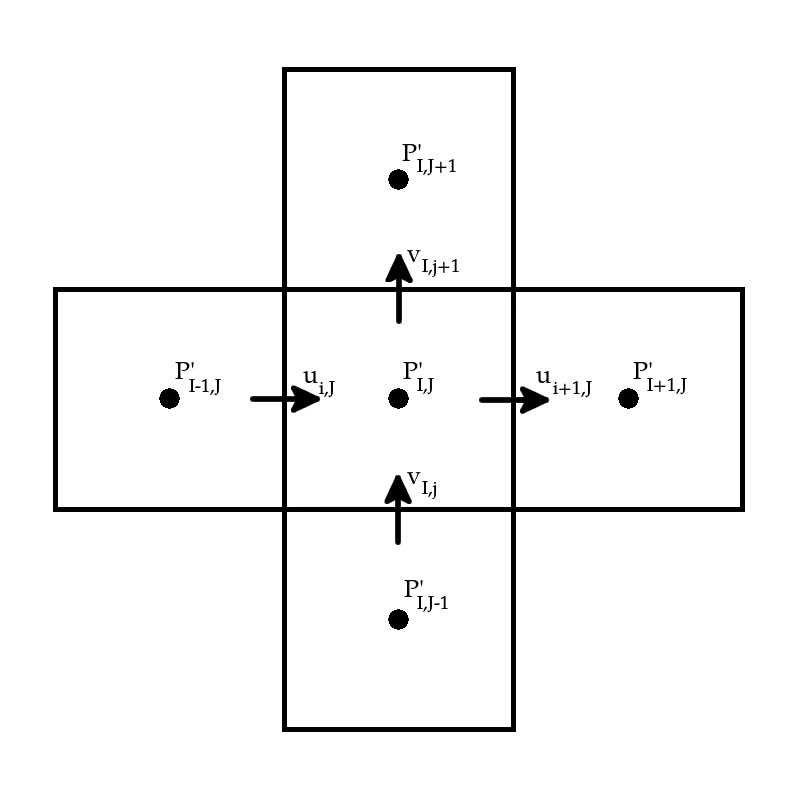
\includegraphics[width=6cm]{Img/7-5}
  \caption{Elemento de Presión}
  \label{fig:7-5}
\end{figure}
Reorganizando obtenemos:
\begin{eqnarray}
 \left( d_{i+1,J} + d_{i,J} + d_{I,j+1} + d_{I,j} \right) P_{I,J}^\prime - d_{i+1,J} P_{I+1,J}^\prime - d_{i,J} P_{I-1,J}^\prime \nonumber \\
- d_{I,j+1} P_{I,J+1}^\prime - d_{I,j} P_{I,J-1}^\prime = u^*_{i,J} - u^*_{i+1,J} + v^*_{I,j} - v^*_{I,j+1}
  \centering \nonumber
\end{eqnarray}

De esta manera a partir de la ecuación de continuidad obtenemos la ecuación para corregir la presión $P^\prime$. Una vez calculada $P^\prime$ podemos resolver las ecuaciones de corrección (\ref{eq:correccionp}, \ref{eq:correccionu} y \ref{eq:correccionv}) y obtener los campo de velocidades y presión corrector.

La corrección de la presión es muy susceptible a la divergencia por lo que se necesita una relajación utilizando un coeficiente.
\begin{equation}
 P_{n+1} = P_n^* + \alpha_p P_{n+1}^\prime
\end{equation}
Donde $\alpha_p$ is la relajación para la corrección de la presión.
\begin{figure}[h!]
  \centering
  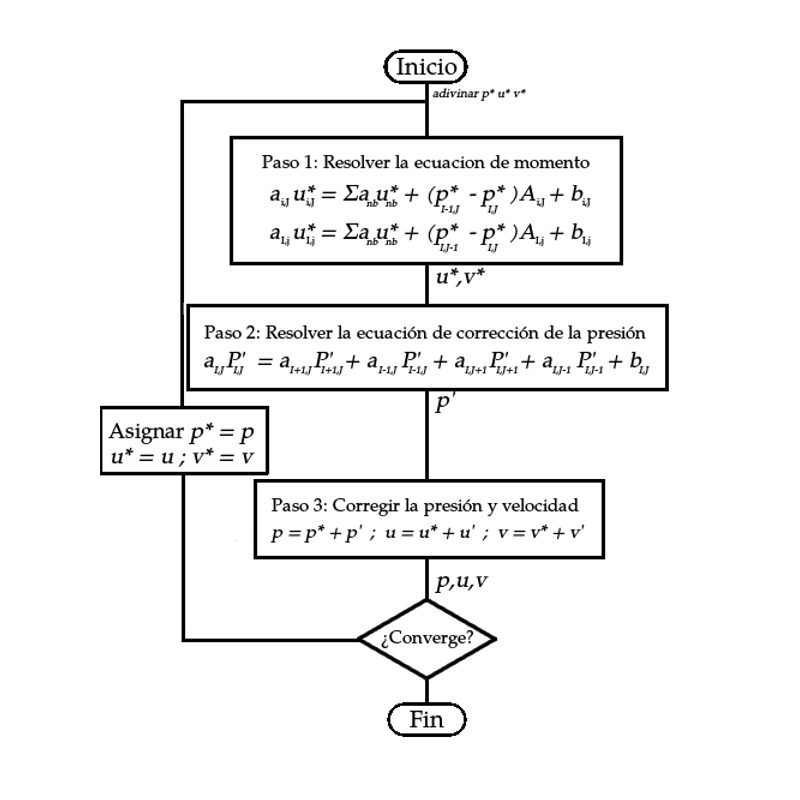
\includegraphics[width=8cm]{Img/7-7}
  \caption{Diagrama de flujo SIMPLE}
  \label{fig:7-7}
\end{figure}


\section{Fractional-Step}

El método Fractional-Step es un esquema de integración temporal que propone descomponer el campo vectorial de velocidades en dos campos ortogonales, uno de gradientes (presión) y un campo vectorial libre de divergencia. La velocidad está formada por la única combinación lineal de estos dos anteriores, tal como se puede observar en la \ref{fig:7-6} imagen.
\begin{figure}[hbt]
  \centering
  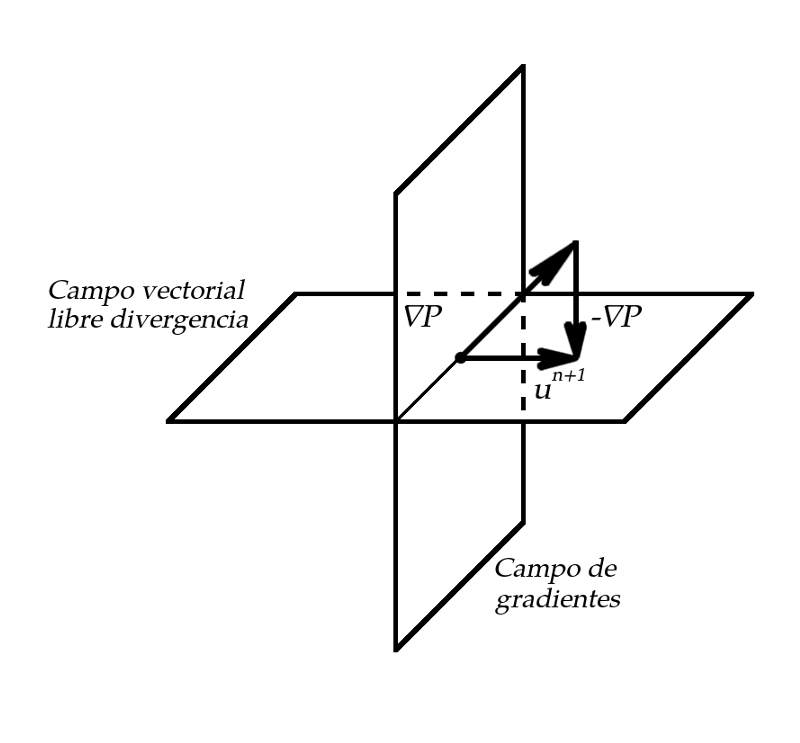
\includegraphics[width=8cm]{Img/7-6}
  \caption{Campo de presión y libre divergencia}
  \label{fig:7-6}
\end{figure}
Con el objetivo de desacoplar los campos de presión y de velocidad, el método calcula un campo predictor ($u^{1+1/2}$) proyectando la ecuación de Navier-Stokes al campo de gradientes donde $\nabla P$ es nula (eq: \ref{eq:prediccion}), este paso intermedio el flujo no cumple con la condición de incompresibilidad y se debe corregir. Para ello, utilizamos el campo de presión para proyectarlo sobre el campo vectorial libre de divergencias, esto se logra restando los campos (eq:\ref{eq:proyeccion}). Para resolver la ecuación de proyección, aplicamos la divergencia en ambos términos para obtener la ecuación de \textit{Poisson}, done el campo de velocidad correcto que si cumple con la condición de incompresibilidad se anula y permite calcular el campo de presión necesario para corregir la velocidad (eq: \ref{eq:correccion}).

\subsection{Algoritmo Fractional-Step}

Comenzamos el desarrolla partiendo de la ecuación de Navier-Stokes, proyectándola sobre el campo de gradientes y de esta manera obtener la ecuación de predicción ($n+1/2$):
\begin{equation}
  \frac{(u^{n+1/2} - u^n)}{\partial t} + \nabla (u^{n+1/2} \cdot u^n ) - \nabla \cdot (\nu \nabla u^{n+1/2}) = - \nabla p^n + S^n.
  \label{eq:prediccion}
\end{equation}
El campo de predicción obtenido al resolver la ecuación anterior no cumple con la condición de incompresibilidad, en consecuencia el campo debe ser sometido a una corrección, es decir, realizar la combinación lineal con el campo vectorial libre de divergencias obtenemos la Proyección corrección:
\begin{equation}
 \frac{u^{n+1} - u^{n+1/2}}{\partial t} = - \nabla (p^{n+1} - p^n).
 \label{eq:proyeccion}
\end{equation}
Se observa que para corregir el campo de velocidad predictor debemos obtener el nuevo campo de presión, esto se logra aplicando la divergencia en ambos términos,
\begin{equation}
 \nabla \cdot u^{n+1} - \nabla \cdot u^{n+1/2} = - \delta t \Delta (p^{n+1} - p^n), \nonumber
\end{equation} 
para obtener la ecuación de Poisson la cual genera un sistema entre los campos ortogonales expresados en la siguiente ecuación:
\begin{equation}
 \delta t \Delta p^{n+1}  =  \nabla \cdot u^{{n+1/2}} + \delta t \Delta p^n. \nonumber
 \label{eq:correccion}
\end{equation}

Para resolver la ecuación integramos en el elemento y aplicamos el teorema de la divergencia:
\begin{equation}
	\delta t \oint \nabla p^{n+1} \cdot \mathbf{n} dS = \oint u^{n+1/2} \cdot \mathbf{n} dS + \delta t  \oint \nabla p^n \cdot \mathbf{n} dS . \nonumber
\end{equation}
Discretizando la integral utilizando la regla del punto medio, con una primera derivada centrada y sumando las fronteras obtenemos:
\begin{equation}
	\sum a_n p^{n+1}_n - a_P p^{n+1}_P = \sum u^{n+1/2}_n \cdot \mathbf{n}_n dS + \sum a_n p^{n}_n - a_P p^{n}_P, \nonumber
\end{equation}
donde el subíndice $n$ hace referencia a la frontera que comparte con el vecino $n$, $a_n = dS / (\mathbf{x}_n - \mathbf{x}_P)$ y $a_P = \sum_n a_n$. Al resolver el sistema obtenemos el campo de presión que necesitamos para hacer la corrección, esta depende del elemento que se esté utilizando, para cuadrados con malla stareged:
\begin{equation}
	u^{n+1} = u^{n+1/2} - \delta t \frac{[(P^{n+1}_E - P^{n+1}_P) - (P^n_E - P^n_P)]}{ \mathbf{x}_E - \mathbf{x}_P}. \nonumber
\end{equation}
Para elementos triangulares se corrige utilizando una propiedad de los triángulos que es:
\begin{equation}
	\sum \mathbf{n}_n \cdot \mathbf{u} ~ l_n= 0, \nonumber 
\end{equation}
siendo $\mathbf{u}$ un vector arbitrario y $l_n$ la longitud de la arista $n$. De esta manera tenemos tres ecuaciones para dos incógnitas, armamos el sistema con las dos primeras y definimos a $u^{n+1}$ como:
\begin{equation}
	u^{n+1} = 
	\begin{bmatrix}
		a_1 \\
		a_2	
	\end{bmatrix},
\end{equation}
por lo tanto el sistema queda:
\begin{equation}
	\begin{bmatrix}
		\mathbf{n}_x^1 & \mathbf{n}_y^1 \\
		\mathbf{n}_x^2 & \mathbf{n}_y^2
	\end{bmatrix}
	\begin{bmatrix}
		a_1 \\
		a_2
	\end{bmatrix}
	=
	\begin{bmatrix}
		\mathbf{n}^1 \cdot \mathbf{u}^{n + 1/2} - [(p^{n+1}_{N_1} - p^{n+1}_p) - (p^n_{N_1} - p^n_p)] /( \mathbf{x}_{N_1} -  \mathbf{x}_P) \\
		\mathbf{n}^2 \cdot \mathbf{u}^{n + 1/2} - [(p^{n+1}_{N_2} - p^{n+1}_p) - (p^n_{N_2} - p^n_p)] /( \mathbf{x}_{N_2} -  \mathbf{x}_P)
	\end{bmatrix}. \nonumber
\end{equation}
Al resolver el sistema de 2x2 obtenemos la velocidad $\mathbf{u}^{n+1}$.

\begin{figure}[h!]
  \centering
  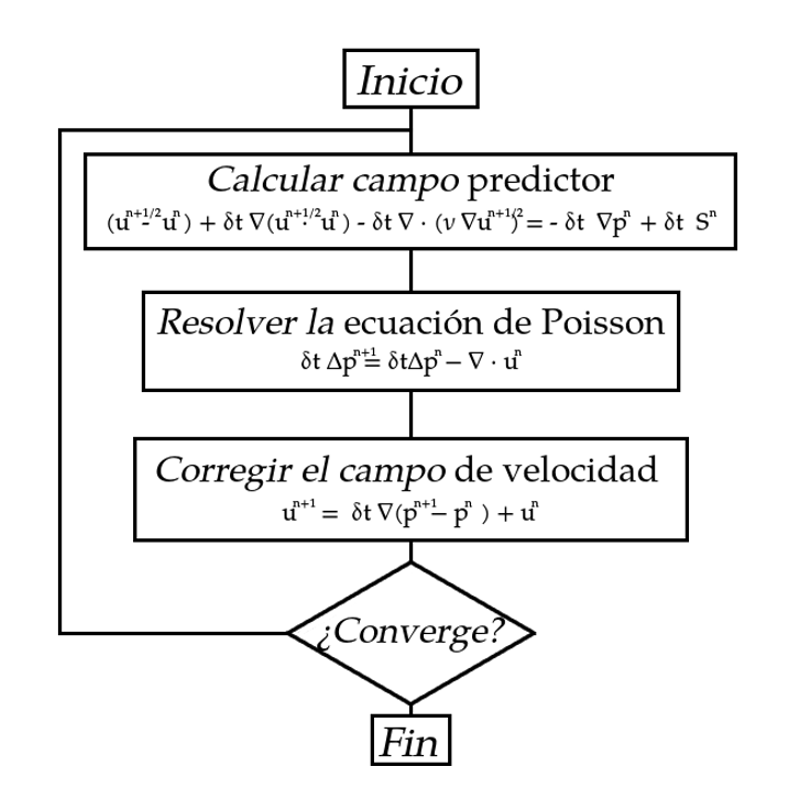
\includegraphics[width=9cm]{Img/7-8}
  \caption{Diagrama de Flujo FSM}
\end{figure}

\chapter{Problem-Type}

El algoritmo desarrollado en este Proyecto Final de Carrera, se califica como un módulo de cálculo que implementa el método de Volúmenes Finitos para la resolución de las ecuaciones de Navier-Stokes para un fluido newtoniano e incompresible desacoplando los campos de presión y velocidad utilizando los métodos SIMPLE y Fractional-Step, en dos dimensiones haciendo uso de mallas estructuradas para elementos cuadrados y no estructuradas para elementos triangulares respectivamente. El ser un módulo de cálculo, implica la dependencia respecto a otro software con el cual interactua para cumplir con su función. Dicha dependencia surge ante la necesidad de un software preparado para generar los datos requeridos para realizar la simulación y la visualización de los resultados obtenidos luego del cálculo, es decir, una herramienta que permita el pre-proceso y el post-proceso.
\begin{figure}[h!]
  \centering
  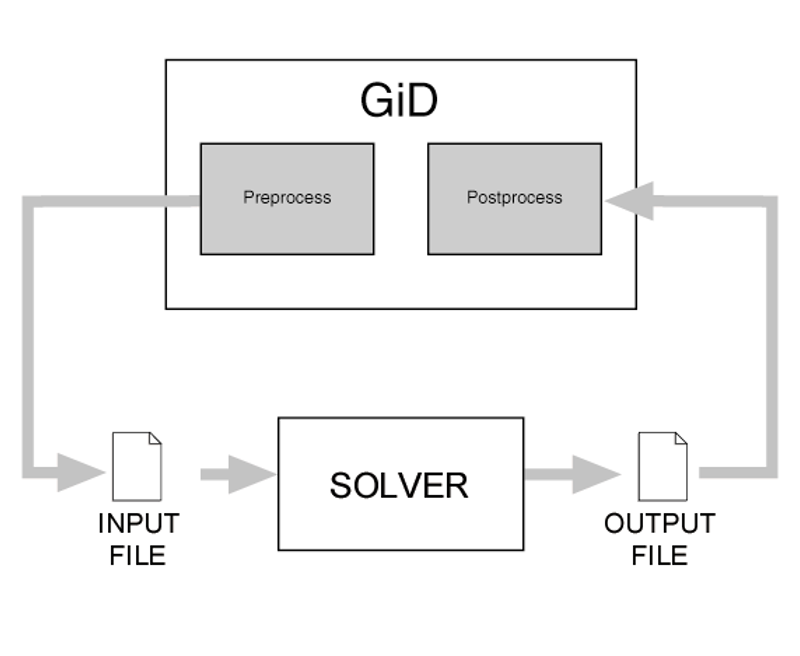
\includegraphics[width=8cm]{Img/8-1}
  \caption{Diagrama de Flujo GiD}
  \label{fig:flujoGiD}
\end{figure}

La herramienta de pre-proceso y el post-proceso utilizada en este trabajo fue proporcionada por el Aula FICH-CIMNE de la Facultad de Ingeniería y Ciencias Hídricas de la Universidad Nacional del Litoral; el software GiD. ``GiD" $~$ es una interfaz gráfica interactiva utilizada para la definición, preparación y visualización de todos los datos relacionados a una simulación numérica. Este conjunto de datos incluye la definición de la geometría, materiales, condiciones, información de la solución y otros parámetros. El programa puede generar una malla adecuada para una gran cantidad de métodos numéricos (elementos finitos, volúmenes o diferencias finitas métodos basados en partículas o métodos sin malla) y puede escribir la información para un programa de simulación numérica en su formato deseado. También es posible ejecutar dichas simulaciones numéricas dentro de GiD y luego utilizarlo para visualizar el resultado del análisis.” \cite{GiD}

Gid proporciona diversas herramientas que son útiles para el pre-proceso, etapa que ejecuta las tareas necesarias para definir el problema:
\begin{itemize}
  \item[$\bullet$] Definir la geometría a trabajar imitando un modelo similar a un CAD (Diseño Asistido por Computadora) con ventaja de que su construcción es de manera jerárquica, lo que implica niveles según la entidad elegida, punto(1), líneas(2), superficies(3) y volúmenes(4).
  \item[$\bullet$] Aplicar las condiciones y atributos del dominio generado seleccionando entre las diferentes condiciones definidas, tales como velocidad impuesta, pared y presión impuesta.
  \item[$\bullet$] Generar la malla asociando los elementos con las condiciones asignadas brindando la posibilidad de elegir el tipo de elemento (triángulos, cuadrados, tetraedros y etc) de manera estructurada o no-estructurada, su refinamiento, entre otras.
\end{itemize}

Al finalizar la etapa de pre-proceso, GiD recopila toda la información del problema planteado y la deriva al módulo de cálculo desarrollado en un formato legible para su buena interpretación. Es en este momento que comienza la tarea del módulo de cálculo, el cual tiene la capacidad de interpretar el problema planteado en el pre-proceso, obtener una solución y generar un archivo con los resultados obtenidos utilizando un formato que interprete GiD, con el objeto de visualizarlos en la etapa de post-proceso.

“GiD utiliza herramientas de visualización avanzada (vista estereoscópica, uso de sombreados, efecto espejo, etc.) en orden de proveer al usuario con el mejor modelo de visualización y obtener un mayor entendimiento de la geometría del modelo o de los resultados de la simulación. Además, permite exportar imágenes y animaciones del modelo en varios formatos, utilizando cualquier modo de visualización e incluyendo resultados.” \cite{GiD}

Este conjunto de etapas ligadas a un módulo de cálculo diseñado para GiD se denomina \textit{problema tipo} (problem type). GiD en su manual define al problema tipo de la siguiente manera:

``El desarrollo de un problema tipo involucra la creación de un directorio con el nombre del problema tipo y la extensión .gid. Este directorio puede ser ubicado en el directorio de trabajo o en el directorio principal de GiD. La serie de archivos de configuración debe estar dentro del directorio del problema tipo. El nombre de la mayoría de ellos seguirá el formato `\textit{problem\_{type}\_{name.xxx}}' , donde la extensión refiere a su función particular. Considerando que el nombre del problema tipo es \textit{problem\_{type}\_{name}} y \textit{project\_{name}} es el nombre del proyecto, la configuración de archivos es descripta por el diagrama de la figura \ref{fig:problematipoGiD}. 
\begin{figure}[h!]
  \centering
  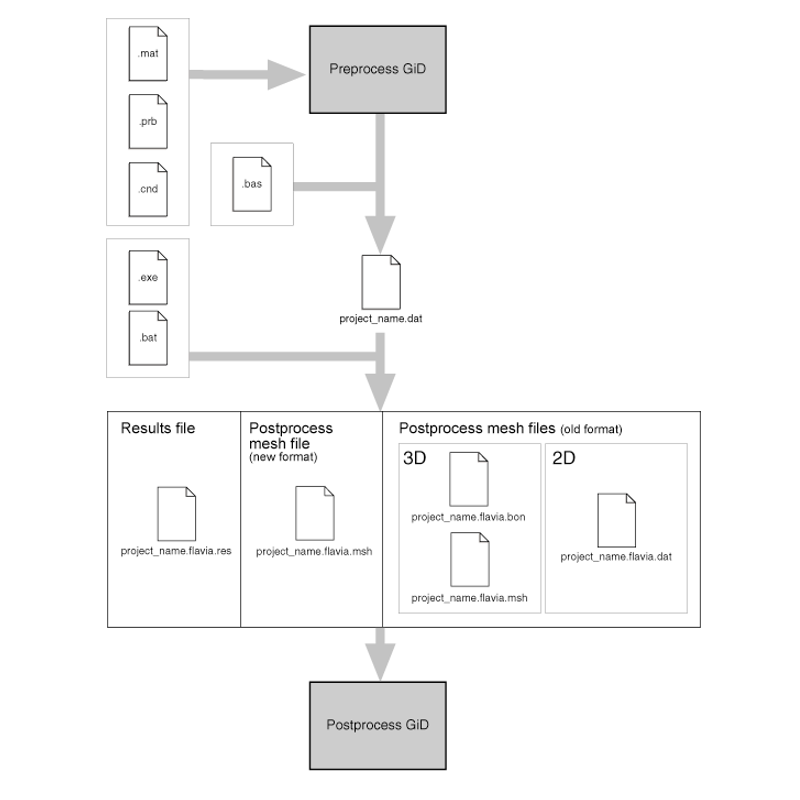
\includegraphics[width=8cm]{Img/8-2}
  \caption{Configuración de Archivos}
  \label{fig:problematipoGiD}
\end{figure}
\begin{itemize}
  \item[$\bullet$] Nombre del Directorio: \textit{problem\_{type}\_{name.gid}}.
  \item[$\bullet$] Ubicación del Directorio: \textit{directorio\_{de}\_{GiD}\textbackslash problemtypes}.
\end{itemize}

\vspace*{0.25in}

\begin{Large}
  \textbf{Archivos de configuración}
\end{Large}

\begin{itemize}
  \item[$\bullet$] \textit{problem\_{type}\_{name.xml}} Configuración basada en XML.
  \item[$\bullet$] \textit{problem\_{}type\_{}name.cnd} Definición de condiciones.
  \item[$\bullet$] \textit{problem\_{}type\_{}name.mat} Propiedades de los materiales.
  \item[$\bullet$] \textit{problem\_{}type\_{}name.prb} Datos del problema e intervalos.
  \item[$\bullet$] \textit{problem\_{}type\_{}name.uni} Sistema de unidades.
  \item[$\bullet$] \textit{problem\_{}type\_{}name.sim} Símbolos de las condiciones.
  \item[$\bullet$] \textit{***.geo} Definición de símbolos geométricos.
  \item[$\bullet$] \textit{***.geo} Definición de símbolos geométricos ...
\end{itemize}

\vspace*{0.25in}

\begin{Large}
  \textbf{Archivos de plantilla}
\end{Large}

\begin{itemize}
  \item[$\bullet$] \textit{problem\_{}type\_{}name.bas} Configuración del archivo de datos de entrada.
  \item[$\bullet$] \textit{***.bas} Información para archivos adicionales.
  \item[$\bullet$] \textit{***.bas} Información para archivos adicionales ...
  \vspace*{0.2in}
  \item[$\bullet$] \textit{Tcl} extension files
  \item[$\bullet$] \textit{problem\_{}type\_{}name.tcl} Extensiones a GiD escritas en lenguaje de programación Tcl/Tk
\end{itemize}

\textbf{Archivos de ejecución de comandos}

\begin{itemize}
  \item[$\bullet$] \textit{problem\_{}type\_{}name.bat} Shell de Sistema Operativo que ejecuta el proceso de
análisis
\end{itemize}

Los archivos \textit{problem\_{}type\_{}name.sim}, \textit{***.geo} and \textit{***.bas} no son obligatorios y pueden ser añadidos para facilitar la visualización (ambos tipos de archivo) o para preparar los datos de entrada para reiniciar en archivos adicionales (solo los archivos \textit{***.bas}). De la misma manera, \textit{problem\_{}type.xml} no es necesario; este puede ser usado para personalizar características como: información de la versión, identificación de íconos, contraseña de validación, etc." \cite{GiD}

Haciendo un enfoque en lo que es requerido por el pre y post-proceso del módulo de cálculo desarrollado, detallaremos las características que contiene el problema tipo:
\begin{itemize}
  \item[$\bullet$] Menú de selección del Sistema de Unidades, permite seleccionar el Sistema Internacional y Imperial, y permite personalizar un Sistema.
  \item[$\bullet$] Menú de definición de Datos del Problema, define pautas de corte tales como la tolerancia de error entre la iteración $i$ y $i-1$, la cantidad de iteraciones máximas, como también el paso de tiempo ($dt$) y el número de Reynolds con el que se quiere trabajar.
  \item[$\bullet$] Menú de definición y asignación de Condiciones, establece las condiciones de contorno sobre la geometría. Tales como: velocidad impuesta, pared y presión impuesta.
  \item[$\bullet$] Ventana de definición y asignación de Materiales, donde el usuario puede definir entre los materiales almacenados o crear uno.
  \item[$\bullet$] Realizar el mallado.
  \item[$\bullet$] Ejecutar el módulo de cálculo.
  \item[$\bullet$] Visualización de los resultados utilizando las herramientas proporcionadas por GiD.
\end{itemize}

$GiD$ Propone generar un directorio para el problema tipo en el cual se encuentran varios archivos, los cuales tienen diferentes funciones:
\begin{itemize}
  \item[$\bullet$] $.pbr$. Brinda información sobre el estado de las variables globales del problema, ya sea la cantidad de 	iteraciones, la densidad del material, el paso del tiempo, entre otras.	
  \item[$\bullet$] $.uni$. Es el archivo que contiene las unidades para las diferentes variables y las relaciona, es decir, para el caso de la velocidad puede ser medida en $m/s$ o $Km/h$ con una relación del $1$ a $3.6$ para mantener la igualdad.
  \item[$\bullet$] $.cnd$. Establece las condiciones de contorno que pueden ser utilizadas en el problema tipo, el cual establece el tipo de condición, el valor y sobre que elemento de la malla se aplica.
  \item[$\bullet$] $.bas$. Su función es generar el archivo $.dat$ utilizando una secuencia de funciones propias de $GiD$ como por ejemplo $*npoin$, que retorna la cantidad de puntos en la malla. La secuencia $*loop nodes *nodes coord(1,real) *end nodes$ retorna el valor de coordenada $x$ para todos los nodos de la malla.
  \item[$\bullet$] $.dat$. Es el archivo de entrada al módulo de calculo, el cual es generado por $GiD$ basado en la secuencia escrita en $.bas$, de esta manera el módulo de calculo lee toda la información, como los nodos, elementos y condiciones de contorno para luego ejecutarse y generar resultados.
  \item[$\bullet$] $.post.res$. Es el archivo generado por el módulo de calculo, el cual será leído por $GiD$ para el post-proceso, es decir, la visualización de los resultados que proporcionó el módulo.
  \item[$\bullet$] $.bat$. Le indica a $GiD$ cual es el ejecutable al que le debe pasar el $.dat$ para que el módulo pueda comenzar con la ejecución, cuales son los archivos $.log$, limpiar archivos viejos que pueden perjudicar el cálculo, entre otras.
  \item[$\bullet$] $.log$. Son archivos que permiten la visualizar al usuario el estado en la ejecución del módulo.
\end{itemize}

\chapter{Resultados}

Resulta necesario corroborar que los métodos implementados funcionan correctamente independientemente de la geometría y del tipo de fluido que se está simulando, debido a esto, surgieron en la Mecánica de Fluidos modelos de validación, los cuales se definen con geometrías sencillas y condiciones de contornos que permitan estimar el comportamiento real del fluido. Definido el modelo de validación, los resultados con los cuales se deben comparar y de esta manera asegurar el correcto funcionamiento del método, son obtenidos a partir de experimentos físicos realizado en laboratorios en condiciones óptimas. Entre la diversidad de los modelos de validación destacaremos el \textit{Lid Driven Cavity} ... Los cuales serán utilizados en este trabajo para validar los resultados obtenidos por los métodos implementados utilizando fluidos con diversos números de \textit{Reynold}.

\section{Lid Driven Cavity}

El modelo de validación Lid Driven Cavity (Figura \ref{img:9-1}) consiste de un fluido dentro de una cavidad cuadrada de $1m$x$1m$ con una placa en la cara superior, la cual se desplaza a una velocidad $u_{m \acute{a} x}$ (imagen ) provocando un vórtice en el centro de la cavidad y según el número de Reynolds que caracteriza al fluido se producen otros vórtices de diferentes tamaños en las esquinas.
\begin{figure}[h!]
	\centering
	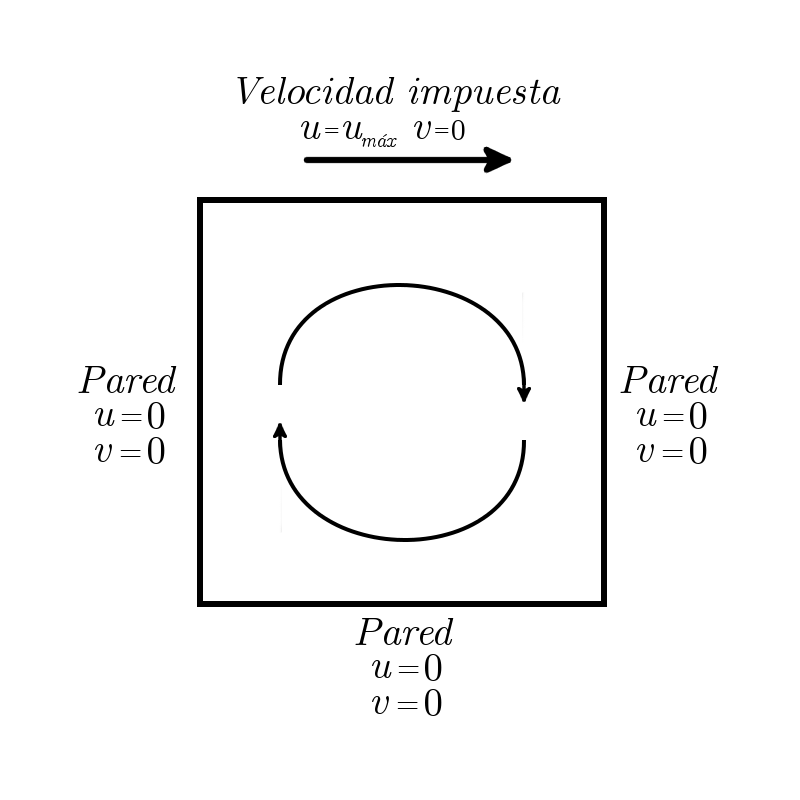
\includegraphics[width=8cm]{Img/9-1}
	\caption{Lid Driven Cavity}
	\label{img:9-1}
\end{figure}

Utilizando como referencia los resultados obtenidos por \textit{Ghia y Shin} en su paper ``\textit{High-Re Solutions for Incompressible Flow Using the Navier-Stokes Equations Multigrid Method}", donde los autores utilizaron una malla estructurada con elementos cuadrados, dividiendo la cavidad en 129x129 nodos. Para extraer los valores obtenidos realizaron dos cortes en la cavidad, el primer corte vertical  es  desde el punto $(0.5;0.0)$ hasta $(0.5;1.0)$ para la componente de velocidad en $u$, el segundo corte es horizontal desde el punto $(0.0;0.5)$ hasta $(1.0;0.5)$ para $v$.

\pagebreak

\subsection{Resultados SIMPLE}

asdf

\subsubsection{Re 100}

asdf

\subsubsection{Re 400}

\subsubsection{Re 1000}

\subsubsection{Re 3200}

\subsection{Resultados Fractional Step}

asdf

\subsubsection{Re 100}

asdf

\subsubsection{Re 400}

\subsubsection{Re 1000}

\subsubsection{Re 3200}

\chapter{Conclusiones}



\bibliography{informe}


\end{document}




